\pdfoutput=1
\documentclass[11pt, a4paper]{article}

% -------------------------------------------------------------------------
% PACKAGES
% -------------------------------------------------------------------------
\usepackage[utf8]{inputenc}
\usepackage{amsmath}
\usepackage{hyphenat} 
\usepackage{amsfonts, amssymb}
\usepackage{geometry}
\usepackage{microtype}
\usepackage{booktabs}
\usepackage{graphicx}
\usepackage{tikz}
\usepackage{pgfplots}
\usepackage{float}
\usepackage{fancyhdr}
\usepackage{xurl}
\usepackage{longtable}
\usepackage{authblk}
\usepackage{threeparttable}
\usepackage{pdflscape}
\usepackage[table]{xcolor}
\usepackage{subcaption}
\usepackage{parskip} 
\usepackage{hyperref}
\usetikzlibrary{arrows.meta, decorations.pathmorphing, plotmarks, shapes.geometric, positioning, calc}
\pgfplotsset{compat=1.18}
\geometry{margin=1in, headheight=14.5pt}
\newcommand{\doi}[1]{\href{https://doi.org/#1}{DOI: #1}}
\usepackage[font=it,labelfont=bf]{caption}

\makeatletter
\setlength{\@fptop}{0pt}
\makeatother

% -------------------------------------------------------------------------
% HEADER & FOOTER (exact template style)
% -------------------------------------------------------------------------
\pagestyle{fancy}
\fancyhf{}
\lhead{Mechanistic Physics}
\rhead{Marab\={u}t's Theory of Gravity: Manuscript 10 Version 1}
\cfoot{\thepage}

% -------------------------------------------------------------------------
% TITLE & AUTHOR
% -------------------------------------------------------------------------
\title{\textbf{Marab\={u}t's Theory of Gravity: \\ The Illusion of the Singularity} \\[1em] \large{The EVGS Grand Ledger and the Final Parsec Problem}}

\author[1]{Christopher Berry Marab\={u}t\thanks{ORCID iD: \href{https://orcid.org/0009-0001-9759-9587}{0009-0001-9759-9587} | Email: chris.marabut@nestlink.com}}
\author[1]{Angelina Lopez Marab\={u}t\thanks{ORCID iD: \href{https://orcid.org/0009-0007-9937-6145}{0009-0007-9937-6145} | Email: angelina.marabut@nestlink.com}}

\affil[1]{Independent Researchers}

\date{May 11, 2026 \\[1.5em] \small{DOI: \url{https://doi.org/10.5281/zenodo.20135534} $|$ Manuscript 10 Version 1}}

\begin{document}

\hypersetup{
  pdftitle={Marab\={u}t's Theory of Gravity: The Illusion of the Singularity},
  pdfauthor={Christopher Berry Marab\={u}t, Angelina Lopez Marab\={u}t},
  pdfkeywords={Marabut's Theory of Gravity, Illusion of the Singularity, EVGS Grand Ledger, Jet Ignition Threshold, Final Parsec Problem, Binary Cascade Superposition, Electron Flow Model, EFM},
  pdfsubject={The EVGS Grand Ledger and the Final Parsec Problem}
}

\maketitle

% -------------------------------------------------------------------------
% ABSTRACT
% -------------------------------------------------------------------------
\begingroup
  \small
  \begin{center}
    \textbf{Abstract}
  \end{center}
  \vspace{-0.5em}

  For over a century, classical astrophysics has been constrained by the illusion of the mathematical singularity—an abstract geometric breakdown where physical laws supposedly collapse. In previous works within this series, the Electron Flow Model (EFM) shattered this illusion by redefining gravity not as a geometric curve, but as Hydrodynamic Fluid Pressure: the literal mechanical drag of the vacuum flux rushing past atomic matter to fill a negative void \cite{marabut2026m1}. Expanding upon principles akin to Superfluid Vacuum Theory (SVT) \cite{sinha1975}, we structurally replaced legacy singularities with physical, calculable thermodynamic entities known as \textbf{Electron Void Gravitational Spheres (EVGS)} \cite{marabut2026m4}. 

  In this tenth manuscript, we provide the definitive empirical proof that the singularity is an illusion by compiling and analyzing the \textit{Marab\={u}t EVGS Master Ledger}—a comprehensive, forward-calculating fluid-dynamic survey of 53 extreme celestial targets, ranging from 1.06 solar masses (SMC X-1) to 66 billion solar masses (TON 618). By anchoring peer-reviewed kinematic data to the EFM framework, we mathematically demonstrate the direct correlation between an EVGS's intrinsic spin, its volumetric fluid intake, and its exhaust ratio. This survey empirically validates a definitive Jet Ignition Threshold at 16\% exhaust ($a^* \approx 0.6$), allowing for the deterministic prediction of relativistic jets based purely on fluid pressure \cite{marabut2026m3, marabut2026m6}. Furthermore, we apply the \textbf{11-point Multiaxial Mara Scale} to map the flow of gravity continuously from the center of the EVGS core (Mara Level 0) to deep space (Mara Level 10). This continuous mapping natively reclassifies ``dormant'' sinks as starving fluid engines and systematically resolves the ``Final Parsec Problem'' \cite{begelman1980} through the fluid friction of Binary Cascade Superposition, proving the cosmos is governed by scalable thermodynamics, not geometric paradoxes.
\endgroup

% -------------------------------------------------------------------------
% TABLE OF CONTENTS
% -------------------------------------------------------------------------
\clearpage
\makeatletter
\renewcommand*\l@subsection{\@dottedtocline{2}{1.5em}{3.2em}} 
\makeatother
\tableofcontents
\clearpage

% -------------------------------------------------------------------------
% 1.0 Introduction: Beyond the Mathematical Singularity
% -------------------------------------------------------------------------
\section{Introduction: Beyond the Mathematical Singularity}
  The traditional cosmological framework is fundamentally constrained by its reliance on the geometric interpretation of General Relativity. When attempting to describe the ultimate sinks of galactic evolution, classical mathematics encounters an insurmountable boundary: the equations yield infinite density and zero volume. Rather than recognizing this as a failure of the geometric model itself, legacy astrophysics codified this mathematical breakdown into a physical entity---the ``singularity''. This forces the assumption that the foundational laws of physics simply cease to function inside an event horizon, creating a century-long paradox.

  Marab\={u}t's Theory of Gravity systematically dismantles this illusion through the fluid-dynamic principles of the Electron Flow Model (EFM). As detailed in \textit{The Push-Pull Mechanics of Vacuum Flux} \cite{marabut2026m1}, the EFM posits that the universe is submerged within an ultra-dense, highly pressurized superfluid electron medium. While this aligns conceptually with Superfluid Vacuum Theory (SVT) \cite{sinha1975}, the EFM introduces a deterministic, macro-scale calculation matrix. Consequently, what legacy models abstractly label as a ``black hole'' is structurally redefined as an \textbf{Electron Void Gravitational Sphere (EVGS)}---a rigid, measurable, three-dimensional engine governed by fluid thermodynamics \cite{marabut2026m8}. 

  As established in \textit{Quantum Mechanics of Stellar Chain Reactions and EVGS Formation} \cite{marabut2026m4}, an EVGS is born when a massive star reaches the end of its lifecycle and collapses. The resulting implosion crushes the atomic lattice into a hyper-dense phase state, stripping away structural buffers and transforming the remnant into a perfect superconductor for vacuum flux ($\tau = 1.000$). This transition creates an ultimate, localized negative sink within the cosmic fluid.

  Gravity, therefore, is redefined natively as Hydrodynamic Fluid Pressure. Crucially, as established in Manuscript 1 \cite{marabut2026m1}, an EVGS does not ``suck'' in surrounding matter like a classical vacuum cleaner. Instead, the persistent existence of this absolute negative sink initiates a massive density imbalance in the universal fluid medium. This triggers the \textbf{Electron Cascade Effect}, where neighboring electrons aggressively rush inward to fill the void, creating a cascading chain reaction of mechanical drag that pulls surrounding atomic structures with it. As demonstrated in our resolution of jet deflection in Cygnus X-1 \cite{marabut2026m3} and the Weyl Potential Anomaly \cite{marabut2026m2}, and further validated across both local heliospheric data \cite{marabut2026m5} and cosmological scales via the kinematic Sunyaev-Zeldovich effect \cite{marabut2026m7}, this fluid-dynamic engine accounts for the most extreme celestial phenomena without requiring the arbitrary warping of spacetime.

  This manuscript serves as the definitive empirical validation of the EFM for these extreme celestial structures. By compiling the \textit{Marab\={u}t EVGS Master Ledger}---a comprehensive survey of 53 distinct EVGS targets utilizing peer-reviewed kinematic data---we apply the EFM mathematical framework to determine the exact structural and mechanical properties of these sinks. The EFM successfully maps this gravitational fluid flow across the entire \textbf{11-point Multiaxial Mara Scale}, charting the continuous pressure gradient from the absolute center of the EVGS core (Mara Level 0) to the far reaches of the deep space boundary (Mara Level 10).

  The survey spans the entire known spectrum of mass and activity, proving that fluid mechanics hold true regardless of cosmological scale. While legacy frameworks, such as the Blandford-Znajek mechanism \cite{blandford1977}, rely on invisible magnetic fields threading a geometric event horizon to extract spin energy, the EFM demonstrates a purely mechanical reality: the intense pressure of the Centrifugal Offset forces a specific percentage of the incoming fluid medium to be violently expelled at the polar extremes. This proves that an EVGS is a functioning engine, and like any engine, its output is dictated by its fuel and rotational resistance. 

  By mathematically quantifying this Exhaust Ratio across all 53 targets, we establish a definitive Jet Ignition Threshold, transforming unpredictable cosmic events into deterministic mechanics. Furthermore, this fluid-dynamic continuum naturally resolves the infamous ``Final Parsec Problem'' \cite{begelman1980, marabut2026m9}, proving that merging supermassive cores generate immense, localized fluid friction without the need for external star scattering. By replacing the illusion of the singularity with empirical fluid thermodynamics, we lay the operational groundwork to systematically dismantle the remaining geometric illusions of legacy cosmology---Dark Matter, Dark Energy, and Spacetime itself.

% -------------------------------------------------------------------------
% 2.0 Methodology and the EFM Mathematical Framework
% -------------------------------------------------------------------------
\section{Methodology and the EFM Mathematical Framework}
To translate standard observational data into EFM mechanics, we utilize a unified mathematical framework. The primary variables extracted from peer-reviewed literature are the EVGS mass ($M$) and its dimensionless relativistic spin parameter ($a^*$). Within the EFM, the dimensionless spin is mapped to a macro-scale 10-point mechanical spin grade ($\Omega_{EFM}$), where $\Omega_{EFM} = a^* \times 10$.

\subsection{Physical Structure and Density}
Unlike classical singularities, an EVGS possesses a rigid, measurable physical volume defined by its radius ($R_{surf}$). Utilizing the established bounds of the classical event horizon as the absolute physical boundary of the void sphere, the radius is calculated natively as:
\begin{equation}
  R_{surf} = \frac{GM}{c^2} \left(1 + \sqrt{1 - a^{*2}}\right)
\end{equation}
Having established a definitive physical volume ($V = \frac{4}{3}\pi R_{surf}^3$), the EFM derives the internal effective density ($\rho_{eff}$) of the sphere:
\begin{equation}
  \rho_{eff} = \frac{M}{V}
\end{equation}
This density calculation is crucial, as it fundamentally dictates the gravitational pull exerted on the surrounding electron fluid medium.

\subsection{Fluid Dynamics: Intake and Exhaust}
The EFM defines gravity not as a geometric warp, but as a literal mechanical pulling force generated by the intake of the fluid medium. The raw Intake Force ($F_{in}$) at the surface of the EVGS (Mara Class 5) is defined by the Marab\={u}t Gravitational Constant ($\alpha_G$), the effective density, and the radius:
\begin{equation}
  F_{in} = \alpha_G \cdot \rho_{eff} \cdot R_{surf} \cdot \tau(T)
\end{equation}
where $\alpha_G \approx 2.792 \times 10^{-7}$ (scaling density in $kg/m^3$ against $R$ in km). Because EVGS cores are ultra-compact and hyper-efficient, they act as perfect superconductors for vacuum flux, yielding a structural impedance of $\tau = 1.000$.

However, the active rotation of the EVGS generates a perpendicular Centrifugal Offset ($C_{off}$), which resists the inward flow of the fluid medium:
\begin{equation}
  C_{off} = \frac{v_{rot}^2}{R_{surf}}
\end{equation}
where $v_{rot} = \frac{a^* \cdot c}{2}$. The true Surface Gravity ($g_{surf}$) is therefore the net difference between the intake mechanism and the rotational resistance:
\begin{equation}
  g_{surf} = \left( F_{in} - C_{off} \right) \cdot \Omega_{shield}
\end{equation}
\textit{Note: As ultimate primary sinks, all EVGS generate their own absolute isolated boundaries, anchoring $\Omega_{shield} = 1.000$.}

Finally, the fundamental breakthrough of the EFM is the quantization of the exhaust mechanism. The intense pressure of the Centrifugal Offset forces a specific percentage of the fluid medium to be violently expelled at the polar extremes, manifesting as relativistic jets. The Exhaust Ratio ($E_{ratio}$) is formulated as:
\begin{equation}
  E_{ratio} = \left(\frac{C_{off}}{F_{in}}\right) \times 100
\end{equation}

% -------------------------------------------------------------------------
% 3.0 Ledger of Calculations: The EVGS Atlas
% -------------------------------------------------------------------------
\clearpage
\section{Ledger of Calculations: The EVGS Atlas}

% -------------------------------------------------------------------------
% Celestial Body 01: 4U 1543-47
% -------------------------------------------------------------------------
\subsection{Celestial Body 01: 4U 1543-47}
This section details the volumetric fluid-dynamic mapping for \textbf{4U 1543-47}, operating within the local medium of Standard interstellar medium. This object has an estimated mass of 9.4 $M_{\odot}$ and a relativistic spin parameter of $a^* = 0.800$ \cite{orosz2002, simbad}.

\vspace{0.5em}
\noindent \textbf{Basic Parameters:}
\begin{itemize}
  \item \textbf{Location:} Milky Way, Lupus constellation
  \item \textbf{Mass:} 9.4 $M_{\odot}$
  \item \textbf{Relativistic Spin Parameter ($a^*$):} 0.800
  \item \textbf{EFM Spin Grade:} 8.0
  \item \textbf{Distance:} 7500.0 pc
  \item \textbf{Local Fluid Medium:} Standard interstellar medium
  \item \textbf{Companion Star:} A-type main-sequence star
  \item \textbf{Companion Mass:} 2.7 $M_{\odot}$
  \item \textbf{Orbital Separation:} 0.06 AU
  \item \textbf{Observed Jets:} Yes, moderate episodic jets.
  \item \textbf{Exhaust Ratio:} 25.63\%
\end{itemize}

\vspace{0.5em}
\noindent \textbf{The Unified Master Equation:}
$$ g_{surf} = \left[ \alpha_G \cdot \rho_{eff} \cdot R_{surf} \cdot \tau(T) - \frac{v_{rot}^2}{R_{surf}} \right] \cdot \Omega_{shield} $$

\vspace{0.5em}
\noindent \textbf{1. Parameters Used in Calculations:}
\begin{center}
  \begin{tabular}{|l|l|}
    \hline
    \textbf{Parameter} & \textbf{Value} \\ \hline
    $\alpha_G$ & $\approx 2.792 \times 10^{-7}$ \\ \hline
    $\rho_{eff}$ & 4.073e+17 \\ \hline
    $R_{surf}$ & 22.21 km \\ \hline
    $\tau(T)$ & 1.000 \\ \hline
    $v_{rot}$ & 1.199e+08 m/s \\ \hline
    intake force & 2.526e+12 m/s$^2$ \\ \hline
    centrifugal offset & 6.475e+11 m/s$^2$ \\ \hline
    $g_{surf}$ & 1.878e+12 m/s$^2$ \\ \hline
    $\Omega_{shield}$ & 1.000 \\ \hline
    Exhaust Ratio & 25.63\% \\ \hline
  \end{tabular}
\end{center}

\vspace{0.5em}
\noindent \textbf{2. Mara Class 5 Surface Anchor Calculation:}
\begin{itemize}
  \item \textbf{Mara Class 5 Surface Gravity ($g_{M5}$):} 1.878e+12 m/s$^2$
  \item \textbf{Vector Point Calculation:} $g_{M5} = 2.526e+12 - 6.475e+11 = 1.878e+12$ m/s$^2$
\end{itemize}

\vspace{0.5em}
\noindent \textbf{3. Mara Vector Points:}
\begin{itemize}
  \item \textbf{Exterior (M6--M10):} Inverse-square scaling outward from event horizon
  \item \textbf{Interior (M4--M0):} Linear compression toward core negative sink
\end{itemize}

\vspace{0.5em}
\noindent \textbf{4. M-Scale 11-Level Volumetric Scan:}
\begin{table}[!ht]
  \centering
  \resizebox{\textwidth}{!}{
    \begin{tabular}{c c c c c c c l}
      \toprule
      \textbf{Level} & \textbf{Radius (km)} & \textbf{$\rho_{eff}$} & \textbf{$\tau$} & \textbf{$g_{EFM}$ (Raw)} & \textbf{EFM $\approx$} & \textbf{NASA Obs} & \textbf{Mechanistic State} \\
      \midrule
      M10 & 44.42 & 0 & 1.000 & 4.696e+11 & 4.696e+11 & $\nexists$ & Deep Space Boundary \\
      M9 & 39.98 & 0 & 1.000 & 5.797e+11 & 5.797e+11 & $\nexists$ & Vacuum Flux Interface \\
      M8 & 35.53 & 0 & 1.000 & 7.337e+11 & 7.337e+11 & $\nexists$ & Upper Intake Zone \\
      M7 & 31.09 & 0 & 1.000 & 9.584e+11 & 9.584e+11 & $\nexists$ & Mid-Orbit Cascade \\
      M6 & 26.65 & 0 & 1.000 & 1.304e+12 & 1.304e+12 & $\nexists$ & Approach Acceleration \\
      \midrule
      \textbf{M5} & \textbf{22.21} & \textbf{4.073e+17} & \textbf{1.000} & \textbf{1.878e+12} & \textbf{1.878e+12} & $\nexists$ & \textbf{Surface (Event Horizon)} \\
      \midrule
      M4 & 17.77 & 4.073e+17 & 1.000 & 2.078e+12 & 2.078e+12 & $\nexists$ & Internal Conduction \\
      M3 & 13.33 & 4.073e+17 & 1.000 & 1.645e+12 & 1.645e+12 & $\nexists$ & Mid-Depth Zone \\
      M2 & 8.88 & 4.073e+17 & 1.000 & 1.212e+12 & 1.212e+12 & $\nexists$ & Peak Flux Density \\
      M1 & 4.44 & 4.073e+17 & 1.000 & 7.217e+11 & 7.217e+11 & $\nexists$ & Near-Core Compression \\
      M0 & 0 & 4.073e+17 & 1.000 & 0 & 0 & 0 & Core Negative Sink \\
      \bottomrule
    \end{tabular}
  }
  \caption{M-Scale 11-Level Volumetric Scan for 4U 1543-47.}
\end{table}

\noindent \textbf{Primary Observational Sources:}
\begin{itemize}
  \item Orosz, J. A. et al. (2002). The Black Hole in the X-Ray Nova 4U 1543-47. The Astrophysical Journal. \cite{orosz2002}
  \item SIMBAD Astronomical Database \cite{simbad}
\end{itemize}

% -------------------------------------------------------------------------
% Celestial Body 02: A0620-00
% -------------------------------------------------------------------------
\clearpage
\subsection{Celestial Body 02: A0620-00}
This section details the volumetric fluid-dynamic mapping for \textbf{A0620-00}, operating within the local medium of Interstellar medium. This object has an estimated mass of 6.6 $M_{\odot}$ and a relativistic spin parameter of $a^* = 0.120$ \cite{cantrell2010, simbad}.

\vspace{0.5em}
\noindent \textbf{Basic Parameters:}
\begin{itemize}
  \item \textbf{Location:} Milky Way, Monoceros constellation
  \item \textbf{Mass:} 6.6 $M_{\odot}$
  \item \textbf{Relativistic Spin Parameter ($a^*$):} 0.120
  \item \textbf{EFM Spin Grade:} 1.2
  \item \textbf{Distance:} 1060.0 pc
  \item \textbf{Local Fluid Medium:} Interstellar medium
  \item \textbf{Companion Star:} K-type main-sequence star
  \item \textbf{Companion Mass:} 0.4 $M_{\odot}$
  \item \textbf{Orbital Separation:} 0.02 AU
  \item \textbf{Observed Jets:} Radio emission detected during outbursts, very faint in quiescence.
  \item \textbf{Exhaust Ratio:} 0.72\%
\end{itemize}

\vspace{0.5em}
\noindent \textbf{The Unified Master Equation:}
$$ g_{surf} = \left[ \alpha_G \cdot \rho_{eff} \cdot R_{surf} \cdot \tau(T) - \frac{v_{rot}^2}{R_{surf}} \right] \cdot \Omega_{shield} $$

\vspace{0.5em}
\noindent \textbf{1. Parameters Used in Calculations:}
\begin{center}
  \begin{tabular}{|l|l|}
    \hline
    \textbf{Parameter} & \textbf{Value} \\ \hline
    $\alpha_G$ & $\approx 2.792 \times 10^{-7}$ \\ \hline
    $\rho_{eff}$ & 4.298e+17 \\ \hline
    $R_{surf}$ & 19.39 km \\ \hline
    $\tau(T)$ & 1.000 \\ \hline
    $v_{rot}$ & 1.799e+07 m/s \\ \hline
    intake force & 2.327e+12 m/s$^2$ \\ \hline
    centrifugal offset & 1.669e+10 m/s$^2$ \\ \hline
    $g_{surf}$ & 2.311e+12 m/s$^2$ \\ \hline
    $\Omega_{shield}$ & 1.000 \\ \hline
    Exhaust Ratio & 0.72\% \\ \hline
  \end{tabular}
\end{center}

\vspace{0.5em}
\noindent \textbf{2. Mara Class 5 Surface Anchor Calculation:}
\begin{itemize}
  \item \textbf{Mara Class 5 Surface Gravity ($g_{M5}$):} 2.311e+12 m/s$^2$
  \item \textbf{Vector Point Calculation:} $g_{M5} = 2.327e+12 - 1.669e+10 = 2.311e+12$ m/s$^2$
\end{itemize}

\vspace{0.5em}
\noindent \textbf{3. Mara Vector Points:}
\begin{itemize}
  \item \textbf{Exterior (M6--M10):} Inverse-square scaling outward from event horizon
  \item \textbf{Interior (M4--M0):} Linear compression toward core negative sink
\end{itemize}

\vspace{0.5em}
\noindent \textbf{4. M-Scale 11-Level Volumetric Scan:}
\begin{table}[!ht]
  \centering
  \resizebox{\textwidth}{!}{
    \begin{tabular}{c c c c c c c l}
      \toprule
      \textbf{Level} & \textbf{Radius (km)} & \textbf{$\rho_{eff}$} & \textbf{$\tau$} & \textbf{$g_{EFM}$ (Raw)} & \textbf{EFM $\approx$} & \textbf{NASA Obs} & \textbf{Mechanistic State} \\
      \midrule
      M10 & 38.79 & 0 & 1.000 & 5.777e+11 & 5.777e+11 & $\nexists$ & Deep Space Boundary \\
      M9 & 34.91 & 0 & 1.000 & 7.132e+11 & 7.132e+11 & $\nexists$ & Vacuum Flux Interface \\
      M8 & 31.03 & 0 & 1.000 & 9.026e+11 & 9.026e+11 & $\nexists$ & Upper Intake Zone \\
      M7 & 27.15 & 0 & 1.000 & 1.179e+12 & 1.179e+12 & $\nexists$ & Mid-Orbit Cascade \\
      M6 & 23.27 & 0 & 1.000 & 1.605e+12 & 1.605e+12 & $\nexists$ & Approach Acceleration \\
      \midrule
      \textbf{M5} & \textbf{19.39} & \textbf{4.298e+17} & \textbf{1.000} & \textbf{2.311e+12} & \textbf{2.311e+12} & $\nexists$ & \textbf{Surface (Event Horizon)} \\
      \midrule
      M4 & 15.51 & 4.298e+17 & 1.000 & 1.916e+12 & 1.916e+12 & $\nexists$ & Internal Conduction \\
      M3 & 11.64 & 4.298e+17 & 1.000 & 1.516e+12 & 1.516e+12 & $\nexists$ & Mid-Depth Zone \\
      M2 & 7.76 & 4.298e+17 & 1.000 & 1.117e+12 & 1.117e+12 & $\nexists$ & Peak Flux Density \\
      M1 & 3.88 & 4.298e+17 & 1.000 & 6.649e+11 & 6.649e+11 & $\nexists$ & Near-Core Compression \\
      M0 & 0 & 4.298e+17 & 1.000 & 0 & 0 & 0 & Core Negative Sink \\
      \bottomrule
    \end{tabular}
  }
  \caption{M-Scale 11-Level Volumetric Scan for A0620-00.}
\end{table}

\noindent \textbf{Primary Observational Sources:}
\begin{itemize}
  \item Cantrell, A. G. et al. (2010). The Inclination of the Soft X-Ray Transient A0620-00 and the Mass of its Black Hole. The Astrophysical Journal. \cite{cantrell2010}
  \item SIMBAD Astronomical Database \cite{simbad}
\end{itemize}

% -------------------------------------------------------------------------
% Celestial Body 03: Centaurus X-3
% -------------------------------------------------------------------------
\clearpage
\subsection{Celestial Body 03: Centaurus X-3}
This section details the volumetric fluid-dynamic mapping for \textbf{Centaurus X-3}, operating within the local medium of Dense stellar wind from O-type supergiant. This object has an estimated mass of 1.21 $M_{\odot}$ and a relativistic spin parameter of $a^* = 0.650$ \cite{rawls2011, simbad}.

\vspace{0.5em}
\noindent \textbf{Basic Parameters:}
\begin{itemize}
  \item \textbf{Location:} Milky Way, Centaurus constellation
  \item \textbf{Mass:} 1.21 $M_{\odot}$
  \item \textbf{Relativistic Spin Parameter ($a^*$):} 0.650
  \item \textbf{EFM Spin Grade:} 6.5
  \item \textbf{Distance:} 5700.0 pc
  \item \textbf{Local Fluid Medium:} Dense stellar wind from O-type supergiant
  \item \textbf{Companion Star:} O-type supergiant (V779 Centauri)
  \item \textbf{Companion Mass:} 20.5 $M_{\odot}$
  \item \textbf{Orbital Separation:} 0.06 AU
  \item \textbf{Observed Jets:} Accretion-powered X-ray pulsar; no prominent continuous jets.
  \item \textbf{Exhaust Ratio:} 18.72\%
\end{itemize}

\vspace{0.5em}
\noindent \textbf{The Unified Master Equation:}
$$ g_{surf} = \left[ \alpha_G \cdot \rho_{eff} \cdot R_{surf} \cdot \tau(T) - \frac{v_{rot}^2}{R_{surf}} \right] \cdot \Omega_{shield} $$

\vspace{0.5em}
\noindent \textbf{1. Parameters Used in Calculations:}
\begin{center}
  \begin{tabular}{|l|l|}
    \hline
    \textbf{Parameter} & \textbf{Value} \\ \hline
    $\alpha_G$ & $\approx 2.792 \times 10^{-7}$ \\ \hline
    $\rho_{eff}$ & 1.841e+19 \\ \hline
    $R_{surf}$ & 3.14 km \\ \hline
    $\tau(T)$ & 1.000 \\ \hline
    $v_{rot}$ & 9.743e+07 m/s \\ \hline
    intake force & 1.614e+13 m/s$^2$ \\ \hline
    centrifugal offset & 3.021e+12 m/s$^2$ \\ \hline
    $g_{surf}$ & 1.312e+13 m/s$^2$ \\ \hline
    $\Omega_{shield}$ & 1.000 \\ \hline
    Exhaust Ratio & 18.72\% \\ \hline
  \end{tabular}
\end{center}

\vspace{0.5em}
\noindent \textbf{2. Mara Class 5 Surface Anchor Calculation:}
\begin{itemize}
  \item \textbf{Mara Class 5 Surface Gravity ($g_{M5}$):} 1.312e+13 m/s$^2$
  \item \textbf{Vector Point Calculation:} $g_{M5} = 1.614e+13 - 3.021e+12 = 1.312e+13$ m/s$^2$
\end{itemize}

\vspace{0.5em}
\noindent \textbf{3. Mara Vector Points:}
\begin{itemize}
  \item \textbf{Exterior (M6--M10):} Inverse-square scaling outward from event horizon
  \item \textbf{Interior (M4--M0):} Linear compression toward core negative sink
\end{itemize}

\vspace{0.5em}
\noindent \textbf{4. M-Scale 11-Level Volumetric Scan:}
\begin{table}[!ht]
  \centering
  \resizebox{\textwidth}{!}{
    \begin{tabular}{c c c c c c c l}
      \toprule
      \textbf{Level} & \textbf{Radius (km)} & \textbf{$\rho_{eff}$} & \textbf{$\tau$} & \textbf{$g_{EFM}$ (Raw)} & \textbf{EFM $\approx$} & \textbf{NASA Obs} & \textbf{Mechanistic State} \\
      \midrule
      M10 & 6.28 & 0 & 1.000 & 3.28e+12 & 3.28e+12 & $\nexists$ & Deep Space Boundary \\
      M9 & 5.65 & 0 & 1.000 & 4.049e+12 & 4.049e+12 & $\nexists$ & Vacuum Flux Interface \\
      M8 & 5.03 & 0 & 1.000 & 5.125e+12 & 5.125e+12 & $\nexists$ & Upper Intake Zone \\
      M7 & 4.4 & 0 & 1.000 & 6.694e+12 & 6.694e+12 & $\nexists$ & Mid-Orbit Cascade \\
      M6 & 3.77 & 0 & 1.000 & 9.111e+12 & 9.111e+12 & $\nexists$ & Approach Acceleration \\
      \midrule
      \textbf{M5} & \textbf{3.14} & \textbf{1.841e+19} & \textbf{1.000} & \textbf{1.312e+13} & \textbf{1.312e+13} & $\nexists$ & \textbf{Surface (Event Horizon)} \\
      \midrule
      M4 & 2.51 & 1.841e+19 & 1.000 & 1.328e+13 & 1.328e+13 & $\nexists$ & Internal Conduction \\
      M3 & 1.88 & 1.841e+19 & 1.000 & 1.051e+13 & 1.051e+13 & $\nexists$ & Mid-Depth Zone \\
      M2 & 1.26 & 1.841e+19 & 1.000 & 7.747e+12 & 7.747e+12 & $\nexists$ & Peak Flux Density \\
      M1 & 0.63 & 1.841e+19 & 1.000 & 4.611e+12 & 4.611e+12 & $\nexists$ & Near-Core Compression \\
      M0 & 0 & 1.841e+19 & 1.000 & 0 & 0 & 0 & Core Negative Sink \\
      \bottomrule
    \end{tabular}
  }
  \caption{M-Scale 11-Level Volumetric Scan for Centaurus X-3.}
\end{table}

\noindent \textbf{Primary Observational Sources:}
\begin{itemize}
  \item Rawls, M. L. et al. (2011). Refined Neutron Star Mass Determinations for Six Eclipsing X-Ray Pulsar Binaries. The Astrophysical Journal. \cite{rawls2011}
  \item SIMBAD Astronomical Database \cite{simbad}
\end{itemize}

% -------------------------------------------------------------------------
% Celestial Body 04: Cyg X-2
% -------------------------------------------------------------------------
\clearpage
\subsection{Celestial Body 04: Cyg X-2}
This section details the volumetric fluid-dynamic mapping for \textbf{Cyg X-2}, operating within the local medium of Standard interstellar medium. This object has an estimated mass of 1.5 $M_{\odot}$ and a relativistic spin parameter of $a^* = 0.400$ \cite{casares2010, simbad}.

\vspace{0.5em}
\noindent \textbf{Basic Parameters:}
\begin{itemize}
  \item \textbf{Location:} Milky Way, Cygnus constellation
  \item \textbf{Mass:} 1.5 $M_{\odot}$
  \item \textbf{Relativistic Spin Parameter ($a^*$):} 0.400
  \item \textbf{EFM Spin Grade:} 4.0
  \item \textbf{Distance:} 8000.0 pc
  \item \textbf{Local Fluid Medium:} Standard interstellar medium
  \item \textbf{Companion Star:} A-type subgiant star
  \item \textbf{Companion Mass:} 0.6 $M_{\odot}$
  \item \textbf{Orbital Separation:} 0.1 AU
  \item \textbf{Observed Jets:} Yes, weak continuous jets.
  \item \textbf{Exhaust Ratio:} 7.68\%
\end{itemize}

\vspace{0.5em}
\noindent \textbf{The Unified Master Equation:}
$$ g_{surf} = \left[ \alpha_G \cdot \rho_{eff} \cdot R_{surf} \cdot \tau(T) - \frac{v_{rot}^2}{R_{surf}} \right] \cdot \Omega_{shield} $$

\vspace{0.5em}
\noindent \textbf{1. Parameters Used in Calculations:}
\begin{center}
  \begin{tabular}{|l|l|}
    \hline
    \textbf{Parameter} & \textbf{Value} \\ \hline
    $\alpha_G$ & $\approx 2.792 \times 10^{-7}$ \\ \hline
    $\rho_{eff}$ & 9.308e+18 \\ \hline
    $R_{surf}$ & 4.25 km \\ \hline
    $\tau(T)$ & 1.000 \\ \hline
    $v_{rot}$ & 5.996e+07 m/s \\ \hline
    intake force & 1.103e+13 m/s$^2$ \\ \hline
    centrifugal offset & 8.469e+11 m/s$^2$ \\ \hline
    $g_{surf}$ & 1.019e+13 m/s$^2$ \\ \hline
    $\Omega_{shield}$ & 1.000 \\ \hline
    Exhaust Ratio & 7.68\% \\ \hline
  \end{tabular}
\end{center}

\vspace{0.5em}
\noindent \textbf{2. Mara Class 5 Surface Anchor Calculation:}
\begin{itemize}
  \item \textbf{Mara Class 5 Surface Gravity ($g_{M5}$):} 1.019e+13 m/s$^2$
  \item \textbf{Vector Point Calculation:} $g_{M5} = 1.103e+13 - 8.469e+11 = 1.019e+13$ m/s$^2$
\end{itemize}

\vspace{0.5em}
\noindent \textbf{3. Mara Vector Points:}
\begin{itemize}
  \item \textbf{Exterior (M6--M10):} Inverse-square scaling outward from event horizon
  \item \textbf{Interior (M4--M0):} Linear compression toward core negative sink
\end{itemize}

\vspace{0.5em}
\noindent \textbf{4. M-Scale 11-Level Volumetric Scan:}
\begin{table}[!ht]
  \centering
  \resizebox{\textwidth}{!}{
    \begin{tabular}{c c c c c c c l}
      \toprule
      \textbf{Level} & \textbf{Radius (km)} & \textbf{$\rho_{eff}$} & \textbf{$\tau$} & \textbf{$g_{EFM}$ (Raw)} & \textbf{EFM $\approx$} & \textbf{NASA Obs} & \textbf{Mechanistic State} \\
      \midrule
      M10 & 8.49 & 0 & 1.000 & 2.546e+12 & 2.546e+12 & $\nexists$ & Deep Space Boundary \\
      M9 & 7.64 & 0 & 1.000 & 3.144e+12 & 3.144e+12 & $\nexists$ & Vacuum Flux Interface \\
      M8 & 6.79 & 0 & 1.000 & 3.979e+12 & 3.979e+12 & $\nexists$ & Upper Intake Zone \\
      M7 & 5.94 & 0 & 1.000 & 5.197e+12 & 5.197e+12 & $\nexists$ & Mid-Orbit Cascade \\
      M6 & 5.09 & 0 & 1.000 & 7.073e+12 & 7.073e+12 & $\nexists$ & Approach Acceleration \\
      \midrule
      \textbf{M5} & \textbf{4.25} & \textbf{9.308e+18} & \textbf{1.000} & \textbf{1.019e+13} & \textbf{1.019e+13} & $\nexists$ & \textbf{Surface (Event Horizon)} \\
      \midrule
      M4 & 3.4 & 9.308e+18 & 1.000 & 9.078e+12 & 9.078e+12 & $\nexists$ & Internal Conduction \\
      M3 & 2.55 & 9.308e+18 & 1.000 & 7.187e+12 & 7.187e+12 & $\nexists$ & Mid-Depth Zone \\
      M2 & 1.7 & 9.308e+18 & 1.000 & 5.295e+12 & 5.295e+12 & $\nexists$ & Peak Flux Density \\
      M1 & 0.85 & 9.308e+18 & 1.000 & 3.152e+12 & 3.152e+12 & $\nexists$ & Near-Core Compression \\
      M0 & 0 & 9.308e+18 & 1.000 & 0 & 0 & 0 & Core Negative Sink \\
      \bottomrule
    \end{tabular}
  }
  \caption{M-Scale 11-Level Volumetric Scan for Cyg X-2.}
\end{table}

\noindent \textbf{Primary Observational Sources:}
\begin{itemize}
  \item Casares, J. et al. (2010). The mass of the neutron star in Cygnus X-2. Monthly Notices of the Royal Astronomical Society. \cite{casares2010}
  \item SIMBAD Astronomical Database \cite{simbad}
\end{itemize}

% -------------------------------------------------------------------------
% Celestial Body 05: Cygnus X-1
% -------------------------------------------------------------------------
\clearpage
\subsection{Celestial Body 05: Cygnus X-1}
This section details the volumetric fluid-dynamic mapping for \textbf{Cygnus X-1}, operating within the local medium of Dense stellar wind environment. This object has an estimated mass of 21.2 $M_{\odot}$ and a relativistic spin parameter of $a^* = 0.998$ \cite{prabu2026, simbad}.

\vspace{0.5em}
\noindent \textbf{Basic Parameters:}
\begin{itemize}
  \item \textbf{Location:} Milky Way, Orion Spur
  \item \textbf{Mass:} 21.2 $M_{\odot}$
  \item \textbf{Relativistic Spin Parameter ($a^*$):} 0.998
  \item \textbf{EFM Spin Grade:} 9.98
  \item \textbf{Distance:} 2200.0 pc
  \item \textbf{Local Fluid Medium:} Dense stellar wind environment
  \item \textbf{Companion Star:} HDE 226868 (Massive O-type supergiant)
  \item \textbf{Companion Mass:} 19.2 $M_{\odot}$
  \item \textbf{Orbital Separation:} 0.2 AU
  \item \textbf{Observed Jets:} Yes, highly powerful, continuous polar jets deflected by the companion's stellar wind (5.2-degree bend).
  \item \textbf{Exhaust Ratio:} 26.51\%
\end{itemize}

\vspace{0.5em}
\noindent \textbf{The Unified Master Equation:}
$$ g_{surf} = \left[ \alpha_G \cdot \rho_{eff} \cdot R_{surf} \cdot \tau(T) - \frac{v_{rot}^2}{R_{surf}} \right] \cdot \Omega_{shield} $$

\vspace{0.5em}
\noindent \textbf{1. Parameters Used in Calculations:}
\begin{center}
  \begin{tabular}{|l|l|}
    \hline
    \textbf{Parameter} & \textbf{Value} \\ \hline
    $\alpha_G$ & $\approx 2.792 \times 10^{-7}$ \\ \hline
    $\rho_{eff}$ & 2.729e+17 \\ \hline
    $R_{surf}$ & 33.28 km \\ \hline
    $\tau(T)$ & 1.000 \\ \hline
    $v_{rot}$ & 1.496e+08 m/s \\ \hline
    intake force & 2.536e+12 m/s$^2$ \\ \hline
    centrifugal offset & 6.724e+11 m/s$^2$ \\ \hline
    $g_{surf}$ & 1.864e+12 m/s$^2$ \\ \hline
    $\Omega_{shield}$ & 1.000 \\ \hline
    Exhaust Ratio & 26.51\% \\ \hline
  \end{tabular}
\end{center}

\vspace{0.5em}
\noindent \textbf{2. Mara Class 5 Surface Anchor Calculation:}
\begin{itemize}
  \item \textbf{Mara Class 5 Surface Gravity ($g_{M5}$):} 1.864e+12 m/s$^2$
  \item \textbf{Vector Point Calculation:} $g_{M5} = 2.536e+12 - 6.724e+11 = 1.864e+12$ m/s$^2$
\end{itemize}

\vspace{0.5em}
\noindent \textbf{3. Mara Vector Points:}
\begin{itemize}
  \item \textbf{Exterior (M6--M10):} Inverse-square scaling outward from event horizon
  \item \textbf{Interior (M4--M0):} Linear compression toward core negative sink
\end{itemize}

\vspace{0.5em}
\noindent \textbf{4. M-Scale 11-Level Volumetric Scan:}
\begin{table}[!ht]
  \centering
  \resizebox{\textwidth}{!}{
    \begin{tabular}{c c c c c c c l}
      \toprule
      \textbf{Level} & \textbf{Radius (km)} & \textbf{$\rho_{eff}$} & \textbf{$\tau$} & \textbf{$g_{EFM}$ (Raw)} & \textbf{EFM $\approx$} & \textbf{NASA Obs} & \textbf{Mechanistic State} \\
      \midrule
      M10 & 66.57 & 0 & 1.000 & 4.66e+11 & 4.66e+11 & $\nexists$ & Deep Space Boundary \\
      M9 & 59.91 & 0 & 1.000 & 5.753e+11 & 5.753e+11 & $\nexists$ & Vacuum Flux Interface \\
      M8 & 53.25 & 0 & 1.000 & 7.281e+11 & 7.281e+11 & $\nexists$ & Upper Intake Zone \\
      M7 & 46.6 & 0 & 1.000 & 9.51e+11 & 9.51e+11 & $\nexists$ & Mid-Orbit Cascade \\
      M6 & 39.94 & 0 & 1.000 & 1.294e+12 & 1.294e+12 & $\nexists$ & Approach Acceleration \\
      \midrule
      \textbf{M5} & \textbf{33.28} & \textbf{2.729e+17} & \textbf{1.000} & \textbf{1.864e+12} & \textbf{1.864e+12} & $\nexists$ & \textbf{Surface (Event Horizon)} \\
      \midrule
      M4 & 26.63 & 2.729e+17 & 1.000 & 2.087e+12 & 2.087e+12 & $\nexists$ & Internal Conduction \\
      M3 & 19.97 & 2.729e+17 & 1.000 & 1.652e+12 & 1.652e+12 & $\nexists$ & Mid-Depth Zone \\
      M2 & 13.31 & 2.729e+17 & 1.000 & 1.217e+12 & 1.217e+12 & $\nexists$ & Peak Flux Density \\
      M1 & 6.66 & 2.729e+17 & 1.000 & 7.247e+11 & 7.247e+11 & $\nexists$ & Near-Core Compression \\
      M0 & 0 & 2.729e+17 & 1.000 & 0 & 0 & 0 & Core Negative Sink \\
      \bottomrule
    \end{tabular}
  }
  \caption{M-Scale 11-Level Volumetric Scan for Cygnus X-1.}
\end{table}

\noindent \textbf{Primary Observational Sources:}
\begin{itemize}
  \item Prabu, S. et al. (2026). A jet bent by a stellar wind in the black hole X-ray binary Cygnus X-1. Nature Astronomy. \cite{prabu2026}
  \item SIMBAD Astronomical Database (Spatial coordinates) \cite{simbad}
\end{itemize}

% -------------------------------------------------------------------------
% Celestial Body 06: Cygnus X-3
% -------------------------------------------------------------------------
\clearpage
\subsection{Celestial Body 06: Cygnus X-3}
This section details the volumetric fluid-dynamic mapping for \textbf{Cygnus X-3}, operating within the local medium of Extremely dense stellar wind from companion. This object has an estimated mass of 2.4 $M_{\odot}$ and a relativistic spin parameter of $a^* = 0.850$ \cite{zdziarski2013, simbad}.

\vspace{0.5em}
\noindent \textbf{Basic Parameters:}
\begin{itemize}
  \item \textbf{Location:} Milky Way, Cygnus constellation
  \item \textbf{Mass:} 2.4 $M_{\odot}$
  \item \textbf{Relativistic Spin Parameter ($a^*$):} 0.850
  \item \textbf{EFM Spin Grade:} 8.5
  \item \textbf{Distance:} 7400.0 pc
  \item \textbf{Local Fluid Medium:} Extremely dense stellar wind from companion
  \item \textbf{Companion Star:} Wolf-Rayet star (helium-rich, massive wind)
  \item \textbf{Companion Mass:} 10.0 $M_{\odot}$
  \item \textbf{Orbital Separation:} 0.03 AU
  \item \textbf{Observed Jets:} Yes, intense microquasar jets strongly affected by the Wolf-Rayet wind.
  \item \textbf{Exhaust Ratio:} 27.61\%
\end{itemize}

\vspace{0.5em}
\noindent \textbf{The Unified Master Equation:}
$$ g_{surf} = \left[ \alpha_G \cdot \rho_{eff} \cdot R_{surf} \cdot \tau(T) - \frac{v_{rot}^2}{R_{surf}} \right] \cdot \Omega_{shield} $$

\vspace{0.5em}
\noindent \textbf{1. Parameters Used in Calculations:}
\begin{center}
  \begin{tabular}{|l|l|}
    \hline
    \textbf{Parameter} & \textbf{Value} \\ \hline
    $\alpha_G$ & $\approx 2.792 \times 10^{-7}$ \\ \hline
    $\rho_{eff}$ & 7.192e+18 \\ \hline
    $R_{surf}$ & 5.41 km \\ \hline
    $\tau(T)$ & 1.000 \\ \hline
    $v_{rot}$ & 1.274e+08 m/s \\ \hline
    intake force & 1.086e+13 m/s$^2$ \\ \hline
    centrifugal offset & 3e+12 m/s$^2$ \\ \hline
    $g_{surf}$ & 7.864e+12 m/s$^2$ \\ \hline
    $\Omega_{shield}$ & 1.000 \\ \hline
    Exhaust Ratio & 27.61\% \\ \hline
  \end{tabular}
\end{center}

\vspace{0.5em}
\noindent \textbf{2. Mara Class 5 Surface Anchor Calculation:}
\begin{itemize}
  \item \textbf{Mara Class 5 Surface Gravity ($g_{M5}$):} 7.864e+12 m/s$^2$
  \item \textbf{Vector Point Calculation:} $g_{M5} = 1.086e+13 - 3e+12 = 7.864e+12$ m/s$^2$
\end{itemize}

\vspace{0.5em}
\noindent \textbf{3. Mara Vector Points:}
\begin{itemize}
  \item \textbf{Exterior (M6--M10):} Inverse-square scaling outward from event horizon
  \item \textbf{Interior (M4--M0):} Linear compression toward core negative sink
\end{itemize}

\vspace{0.5em}
\noindent \textbf{4. M-Scale 11-Level Volumetric Scan:}
\begin{table}[!ht]
  \centering
  \resizebox{\textwidth}{!}{
    \begin{tabular}{c c c c c c c l}
      \toprule
      \textbf{Level} & \textbf{Radius (km)} & \textbf{$\rho_{eff}$} & \textbf{$\tau$} & \textbf{$g_{EFM}$ (Raw)} & \textbf{EFM $\approx$} & \textbf{NASA Obs} & \textbf{Mechanistic State} \\
      \midrule
      M10 & 10.82 & 0 & 1.000 & 1.966e+12 & 1.966e+12 & $\nexists$ & Deep Space Boundary \\
      M9 & 9.74 & 0 & 1.000 & 2.427e+12 & 2.427e+12 & $\nexists$ & Vacuum Flux Interface \\
      M8 & 8.66 & 0 & 1.000 & 3.072e+12 & 3.072e+12 & $\nexists$ & Upper Intake Zone \\
      M7 & 7.58 & 0 & 1.000 & 4.012e+12 & 4.012e+12 & $\nexists$ & Mid-Orbit Cascade \\
      M6 & 6.49 & 0 & 1.000 & 5.461e+12 & 5.461e+12 & $\nexists$ & Approach Acceleration \\
      \midrule
      \textbf{M5} & \textbf{5.41} & \textbf{7.192e+18} & \textbf{1.000} & \textbf{7.864e+12} & \textbf{7.864e+12} & $\nexists$ & \textbf{Surface (Event Horizon)} \\
      \midrule
      M4 & 4.33 & 7.192e+18 & 1.000 & 8.94e+12 & 8.94e+12 & $\nexists$ & Internal Conduction \\
      M3 & 3.25 & 7.192e+18 & 1.000 & 7.077e+12 & 7.077e+12 & $\nexists$ & Mid-Depth Zone \\
      M2 & 2.16 & 7.192e+18 & 1.000 & 5.215e+12 & 5.215e+12 & $\nexists$ & Peak Flux Density \\
      M1 & 1.08 & 7.192e+18 & 1.000 & 3.104e+12 & 3.104e+12 & $\nexists$ & Near-Core Compression \\
      M0 & 0 & 7.192e+18 & 1.000 & 0 & 0 & 0 & Core Negative Sink \\
      \bottomrule
    \end{tabular}
  }
  \caption{M-Scale 11-Level Volumetric Scan for Cygnus X-3.}
\end{table}

\noindent \textbf{Primary Observational Sources:}
\begin{itemize}
  \item Zdziarski, A. A. et al. (2013). The black hole binary Cygnus X-3. Monthly Notices of the Royal Astronomical Society. \cite{zdziarski2013}
  \item SIMBAD Astronomical Database (Spatial coordinates) \cite{simbad}
\end{itemize}

% -------------------------------------------------------------------------
% Celestial Body 07: Gaia BH1
% -------------------------------------------------------------------------
\clearpage
\subsection{Celestial Body 07: Gaia BH1}
This section details the volumetric fluid-dynamic mapping for \textbf{Gaia BH1}, operating within the local medium of Quiet interstellar medium (Halo/Thick Disk transit). This object has an estimated mass of 9.62 $M_{\odot}$ and a relativistic spin parameter of $a^* = 0.000$ \cite{el-badry2023, simbad}.

\vspace{0.5em}
\noindent \textbf{Basic Parameters:}
\begin{itemize}
  \item \textbf{Location:} Milky Way, Ophiuchus constellation
  \item \textbf{Mass:} 9.62 $M_{\odot}$
  \item \textbf{Relativistic Spin Parameter ($a^*$):} 0.000
  \item \textbf{EFM Spin Grade:} 0.0
  \item \textbf{Distance:} 480.0 pc
  \item \textbf{Local Fluid Medium:} Quiet interstellar medium (Halo/Thick Disk transit)
  \item \textbf{Companion Star:} G-type main-sequence star
  \item \textbf{Companion Mass:} 0.93 $M_{\odot}$
  \item \textbf{Orbital Separation:} 1.4 AU
  \item \textbf{Observed Jets:} Completely dormant (no X-ray or radio detection).
  \item \textbf{Exhaust Ratio:} 0.0\%
\end{itemize}

\vspace{0.5em}
\noindent \textbf{The Unified Master Equation:}
$$ g_{surf} = \left[ \alpha_G \cdot \rho_{eff} \cdot R_{surf} \cdot \tau(T) - \frac{v_{rot}^2}{R_{surf}} \right] \cdot \Omega_{shield} $$

\vspace{0.5em}
\noindent \textbf{1. Parameters Used in Calculations:}
\begin{center}
  \begin{tabular}{|l|l|}
    \hline
    \textbf{Parameter} & \textbf{Value} \\ \hline
    $\alpha_G$ & $\approx 2.792 \times 10^{-7}$ \\ \hline
    $\rho_{eff}$ & 1.991e+17 \\ \hline
    $R_{surf}$ & 28.41 km \\ \hline
    $\tau(T)$ & 1.000 \\ \hline
    $v_{rot}$ & 0 m/s \\ \hline
    intake force & 1.58e+12 m/s$^2$ \\ \hline
    centrifugal offset & 0 m/s$^2$ \\ \hline
    $g_{surf}$ & 1.58e+12 m/s$^2$ \\ \hline
    $\Omega_{shield}$ & 1.000 \\ \hline
    Exhaust Ratio & 0.0\% \\ \hline
  \end{tabular}
\end{center}

\vspace{0.5em}
\noindent \textbf{2. Mara Class 5 Surface Anchor Calculation:}
\begin{itemize}
  \item \textbf{Mara Class 5 Surface Gravity ($g_{M5}$):} 1.58e+12 m/s$^2$
  \item \textbf{Vector Point Calculation:} $g_{M5} = 1.58e+12 - 0 = 1.58e+12$ m/s$^2$
\end{itemize}

\vspace{0.5em}
\noindent \textbf{3. Mara Vector Points:}
\begin{itemize}
  \item \textbf{Exterior (M6--M10):} Inverse-square scaling outward from event horizon
  \item \textbf{Interior (M4--M0):} Linear compression toward core negative sink
\end{itemize}

\vspace{0.5em}
\noindent \textbf{4. M-Scale 11-Level Volumetric Scan:}
\begin{table}[!ht]
  \centering
  \resizebox{\textwidth}{!}{
    \begin{tabular}{c c c c c c c l}
      \toprule
      \textbf{Level} & \textbf{Radius (km)} & \textbf{$\rho_{eff}$} & \textbf{$\tau$} & \textbf{$g_{EFM}$ (Raw)} & \textbf{EFM $\approx$} & \textbf{NASA Obs} & \textbf{Mechanistic State} \\
      \midrule
      M10 & 56.82 & 0 & 1.000 & 3.949e+11 & 3.949e+11 & $\nexists$ & Deep Space Boundary \\
      M9 & 51.14 & 0 & 1.000 & 4.875e+11 & 4.875e+11 & $\nexists$ & Vacuum Flux Interface \\
      M8 & 45.46 & 0 & 1.000 & 6.17e+11 & 6.17e+11 & $\nexists$ & Upper Intake Zone \\
      M7 & 39.78 & 0 & 1.000 & 8.059e+11 & 8.059e+11 & $\nexists$ & Mid-Orbit Cascade \\
      M6 & 34.09 & 0 & 1.000 & 1.097e+12 & 1.097e+12 & $\nexists$ & Approach Acceleration \\
      \midrule
      \textbf{M5} & \textbf{28.41} & \textbf{1.991e+17} & \textbf{1.000} & \textbf{1.58e+12} & \textbf{1.58e+12} & $\nexists$ & \textbf{Surface (Event Horizon)} \\
      \midrule
      M4 & 22.73 & 1.991e+17 & 1.000 & 1.3e+12 & 1.3e+12 & $\nexists$ & Internal Conduction \\
      M3 & 17.05 & 1.991e+17 & 1.000 & 1.029e+12 & 1.029e+12 & $\nexists$ & Mid-Depth Zone \\
      M2 & 11.36 & 1.991e+17 & 1.000 & 7.582e+11 & 7.582e+11 & $\nexists$ & Peak Flux Density \\
      M1 & 5.68 & 1.991e+17 & 1.000 & 4.513e+11 & 4.513e+11 & $\nexists$ & Near-Core Compression \\
      M0 & 0 & 1.991e+17 & 1.000 & 0 & 0 & 0 & Core Negative Sink \\
      \bottomrule
    \end{tabular}
  }
  \caption{M-Scale 11-Level Volumetric Scan for Gaia BH1.}
\end{table}

\noindent \textbf{Primary Observational Sources:}
\begin{itemize}
  \item El-Badry, K. et al. (2023). A Sun-like star orbiting a dormant black hole. Monthly Notices of the Royal Astronomical Society. \cite{el-badry2023}
  \item SIMBAD Astronomical Database \cite{simbad}
\end{itemize}

% -------------------------------------------------------------------------
% Celestial Body 08: Gaia BH2
% -------------------------------------------------------------------------
\clearpage
\subsection{Celestial Body 08: Gaia BH2}
This section details the volumetric fluid-dynamic mapping for \textbf{Gaia BH2}, operating within the local medium of Quiet interstellar medium. This object has an estimated mass of 8.9 $M_{\odot}$ and a relativistic spin parameter of $a^* = 0.000$ \cite{el-badry2023, simbad}.

\vspace{0.5em}
\noindent \textbf{Basic Parameters:}
\begin{itemize}
  \item \textbf{Location:} Milky Way, Centaurus constellation
  \item \textbf{Mass:} 8.9 $M_{\odot}$
  \item \textbf{Relativistic Spin Parameter ($a^*$):} 0.000
  \item \textbf{EFM Spin Grade:} 0.0
  \item \textbf{Distance:} 1160.0 pc
  \item \textbf{Local Fluid Medium:} Quiet interstellar medium
  \item \textbf{Companion Star:} Red giant star
  \item \textbf{Companion Mass:} 1.07 $M_{\odot}$
  \item \textbf{Orbital Separation:} 5.0 AU
  \item \textbf{Observed Jets:} Completely dormant.
  \item \textbf{Exhaust Ratio:} 0.0\%
\end{itemize}

\vspace{0.5em}
\noindent \textbf{The Unified Master Equation:}
$$ g_{surf} = \left[ \alpha_G \cdot \rho_{eff} \cdot R_{surf} \cdot \tau(T) - \frac{v_{rot}^2}{R_{surf}} \right] \cdot \Omega_{shield} $$

\vspace{0.5em}
\noindent \textbf{1. Parameters Used in Calculations:}
\begin{center}
  \begin{tabular}{|l|l|}
    \hline
    \textbf{Parameter} & \textbf{Value} \\ \hline
    $\alpha_G$ & $\approx 2.792 \times 10^{-7}$ \\ \hline
    $\rho_{eff}$ & 2.327e+17 \\ \hline
    $R_{surf}$ & 26.28 km \\ \hline
    $\tau(T)$ & 1.000 \\ \hline
    $v_{rot}$ & 0 m/s \\ \hline
    intake force & 1.707e+12 m/s$^2$ \\ \hline
    centrifugal offset & 0 m/s$^2$ \\ \hline
    $g_{surf}$ & 1.707e+12 m/s$^2$ \\ \hline
    $\Omega_{shield}$ & 1.000 \\ \hline
    Exhaust Ratio & 0.0\% \\ \hline
  \end{tabular}
\end{center}

\vspace{0.5em}
\noindent \textbf{2. Mara Class 5 Surface Anchor Calculation:}
\begin{itemize}
  \item \textbf{Mara Class 5 Surface Gravity ($g_{M5}$):} 1.707e+12 m/s$^2$
  \item \textbf{Vector Point Calculation:} $g_{M5} = 1.707e+12 - 0 = 1.707e+12$ m/s$^2$
\end{itemize}

\vspace{0.5em}
\noindent \textbf{3. Mara Vector Points:}
\begin{itemize}
  \item \textbf{Exterior (M6--M10):} Inverse-square scaling outward from event horizon
  \item \textbf{Interior (M4--M0):} Linear compression toward core negative sink
\end{itemize}

\vspace{0.5em}
\noindent \textbf{4. M-Scale 11-Level Volumetric Scan:}
\begin{table}[!ht]
  \centering
  \resizebox{\textwidth}{!}{
    \begin{tabular}{c c c c c c c l}
      \toprule
      \textbf{Level} & \textbf{Radius (km)} & \textbf{$\rho_{eff}$} & \textbf{$\tau$} & \textbf{$g_{EFM}$ (Raw)} & \textbf{EFM $\approx$} & \textbf{NASA Obs} & \textbf{Mechanistic State} \\
      \midrule
      M10 & 52.57 & 0 & 1.000 & 4.268e+11 & 4.268e+11 & $\nexists$ & Deep Space Boundary \\
      M9 & 47.31 & 0 & 1.000 & 5.27e+11 & 5.27e+11 & $\nexists$ & Vacuum Flux Interface \\
      M8 & 42.06 & 0 & 1.000 & 6.669e+11 & 6.669e+11 & $\nexists$ & Upper Intake Zone \\
      M7 & 36.8 & 0 & 1.000 & 8.711e+11 & 8.711e+11 & $\nexists$ & Mid-Orbit Cascade \\
      M6 & 31.54 & 0 & 1.000 & 1.186e+12 & 1.186e+12 & $\nexists$ & Approach Acceleration \\
      \midrule
      \textbf{M5} & \textbf{26.28} & \textbf{2.327e+17} & \textbf{1.000} & \textbf{1.707e+12} & \textbf{1.707e+12} & $\nexists$ & \textbf{Surface (Event Horizon)} \\
      \midrule
      M4 & 21.03 & 2.327e+17 & 1.000 & 1.405e+12 & 1.405e+12 & $\nexists$ & Internal Conduction \\
      M3 & 15.77 & 2.327e+17 & 1.000 & 1.112e+12 & 1.112e+12 & $\nexists$ & Mid-Depth Zone \\
      M2 & 10.51 & 2.327e+17 & 1.000 & 8.195e+11 & 8.195e+11 & $\nexists$ & Peak Flux Density \\
      M1 & 5.26 & 2.327e+17 & 1.000 & 4.878e+11 & 4.878e+11 & $\nexists$ & Near-Core Compression \\
      M0 & 0 & 2.327e+17 & 1.000 & 0 & 0 & 0 & Core Negative Sink \\
      \bottomrule
    \end{tabular}
  }
  \caption{M-Scale 11-Level Volumetric Scan for Gaia BH2.}
\end{table}

\noindent \textbf{Primary Observational Sources:}
\begin{itemize}
  \item El-Badry, K. et al. (2023). A red giant orbiting a black hole. Monthly Notices of the Royal Astronomical Society. \cite{el-badry2023}
  \item SIMBAD Astronomical Database \cite{simbad}
\end{itemize}

% -------------------------------------------------------------------------
% Celestial Body 09: GRO J1655-40
% -------------------------------------------------------------------------
\clearpage
\subsection{Celestial Body 09: GRO J1655-40}
This section details the volumetric fluid-dynamic mapping for \textbf{GRO J1655-40}, operating within the local medium of Passing through the galactic disk at an unusually high speed (a 'runaway' EVGS). This object has an estimated mass of 6.3 $M_{\odot}$ and a relativistic spin parameter of $a^* = 0.700$ \cite{orosz1997, simbad}.

\vspace{0.5em}
\noindent \textbf{Basic Parameters:}
\begin{itemize}
  \item \textbf{Location:} Milky Way, Scorpius constellation
  \item \textbf{Mass:} 6.3 $M_{\odot}$
  \item \textbf{Relativistic Spin Parameter ($a^*$):} 0.700
  \item \textbf{EFM Spin Grade:} 7.0
  \item \textbf{Distance:} 3200.0 pc
  \item \textbf{Local Fluid Medium:} Passing through the galactic disk at an unusually high speed (a 'runaway' EVGS)
  \item \textbf{Companion Star:} F-type subgiant star
  \item \textbf{Companion Mass:} 2.3 $M_{\odot}$
  \item \textbf{Orbital Separation:} 0.12 AU
  \item \textbf{Observed Jets:} Yes, episodic jets.
  \item \textbf{Exhaust Ratio:} 21.03\%
\end{itemize}

\vspace{0.5em}
\noindent \textbf{The Unified Master Equation:}
$$ g_{surf} = \left[ \alpha_G \cdot \rho_{eff} \cdot R_{surf} \cdot \tau(T) - \frac{v_{rot}^2}{R_{surf}} \right] \cdot \Omega_{shield} $$

\vspace{0.5em}
\noindent \textbf{1. Parameters Used in Calculations:}
\begin{center}
  \begin{tabular}{|l|l|}
    \hline
    \textbf{Parameter} & \textbf{Value} \\ \hline
    $\alpha_G$ & $\approx 2.792 \times 10^{-7}$ \\ \hline
    $\rho_{eff}$ & 7.375e+17 \\ \hline
    $R_{surf}$ & 15.95 km \\ \hline
    $\tau(T)$ & 1.000 \\ \hline
    $v_{rot}$ & 1.049e+08 m/s \\ \hline
    intake force & 3.284e+12 m/s$^2$ \\ \hline
    centrifugal offset & 6.904e+11 m/s$^2$ \\ \hline
    $g_{surf}$ & 2.593e+12 m/s$^2$ \\ \hline
    $\Omega_{shield}$ & 1.000 \\ \hline
    Exhaust Ratio & 21.03\% \\ \hline
  \end{tabular}
\end{center}

\vspace{0.5em}
\noindent \textbf{2. Mara Class 5 Surface Anchor Calculation:}
\begin{itemize}
  \item \textbf{Mara Class 5 Surface Gravity ($g_{M5}$):} 2.593e+12 m/s$^2$
  \item \textbf{Vector Point Calculation:} $g_{M5} = 3.284e+12 - 6.904e+11 = 2.593e+12$ m/s$^2$
\end{itemize}

\vspace{0.5em}
\noindent \textbf{3. Mara Vector Points:}
\begin{itemize}
  \item \textbf{Exterior (M6--M10):} Inverse-square scaling outward from event horizon
  \item \textbf{Interior (M4--M0):} Linear compression toward core negative sink
\end{itemize}

\vspace{0.5em}
\noindent \textbf{4. M-Scale 11-Level Volumetric Scan:}
\begin{table}[!ht]
  \centering
  \resizebox{\textwidth}{!}{
    \begin{tabular}{c c c c c c c l}
      \toprule
      \textbf{Level} & \textbf{Radius (km)} & \textbf{$\rho_{eff}$} & \textbf{$\tau$} & \textbf{$g_{EFM}$ (Raw)} & \textbf{EFM $\approx$} & \textbf{NASA Obs} & \textbf{Mechanistic State} \\
      \midrule
      M10 & 31.89 & 0 & 1.000 & 6.483e+11 & 6.483e+11 & $\nexists$ & Deep Space Boundary \\
      M9 & 28.7 & 0 & 1.000 & 8.004e+11 & 8.004e+11 & $\nexists$ & Vacuum Flux Interface \\
      M8 & 25.51 & 0 & 1.000 & 1.013e+12 & 1.013e+12 & $\nexists$ & Upper Intake Zone \\
      M7 & 22.33 & 0 & 1.000 & 1.323e+12 & 1.323e+12 & $\nexists$ & Mid-Orbit Cascade \\
      M6 & 19.14 & 0 & 1.000 & 1.801e+12 & 1.801e+12 & $\nexists$ & Approach Acceleration \\
      \midrule
      \textbf{M5} & \textbf{15.95} & \textbf{7.375e+17} & \textbf{1.000} & \textbf{2.593e+12} & \textbf{2.593e+12} & $\nexists$ & \textbf{Surface (Event Horizon)} \\
      \midrule
      M4 & 12.76 & 7.375e+17 & 1.000 & 2.702e+12 & 2.702e+12 & $\nexists$ & Internal Conduction \\
      M3 & 9.57 & 7.375e+17 & 1.000 & 2.139e+12 & 2.139e+12 & $\nexists$ & Mid-Depth Zone \\
      M2 & 6.38 & 7.375e+17 & 1.000 & 1.576e+12 & 1.576e+12 & $\nexists$ & Peak Flux Density \\
      M1 & 3.19 & 7.375e+17 & 1.000 & 9.382e+11 & 9.382e+11 & $\nexists$ & Near-Core Compression \\
      M0 & 0 & 7.375e+17 & 1.000 & 0 & 0 & 0 & Core Negative Sink \\
      \bottomrule
    \end{tabular}
  }
  \caption{M-Scale 11-Level Volumetric Scan for GRO J1655-40.}
\end{table}

\noindent \textbf{Primary Observational Sources:}
\begin{itemize}
  \item Orosz, J. A., \& Bailyn, C. D. (1997). Optical Observations of the Black Hole Candidate GRO J1655-40. The Astrophysical Journal. \cite{orosz1997}
  \item SIMBAD Astronomical Database (Spatial coordinates) \cite{simbad}
\end{itemize}

% -------------------------------------------------------------------------
% Celestial Body 10: GRS 1915+105
% -------------------------------------------------------------------------
\clearpage
\subsection{Celestial Body 10: GRS 1915+105}
This section details the volumetric fluid-dynamic mapping for \textbf{GRS 1915+105}, operating within the local medium of Extremely dense interstellar gas and dust. This object has an estimated mass of 12.4 $M_{\odot}$ and a relativistic spin parameter of $a^* = 0.980$ \cite{mirabel1994, simbad}.

\vspace{0.5em}
\noindent \textbf{Basic Parameters:}
\begin{itemize}
  \item \textbf{Location:} Milky Way, deep within the galactic plane
  \item \textbf{Mass:} 12.4 $M_{\odot}$
  \item \textbf{Relativistic Spin Parameter ($a^*$):} 0.980
  \item \textbf{EFM Spin Grade:} 9.8
  \item \textbf{Distance:} 8600.0 pc
  \item \textbf{Local Fluid Medium:} Extremely dense interstellar gas and dust
  \item \textbf{Companion Star:} K-type red giant
  \item \textbf{Companion Mass:} 1.2 $M_{\odot}$
  \item \textbf{Orbital Separation:} 0.5 AU
  \item \textbf{Observed Jets:} Yes, famous 'microquasar.' It shoots out massive blobs of plasma at apparent superluminal speeds.
  \item \textbf{Exhaust Ratio:} 28.83\%
\end{itemize}

\vspace{0.5em}
\noindent \textbf{The Unified Master Equation:}
$$ g_{surf} = \left[ \alpha_G \cdot \rho_{eff} \cdot R_{surf} \cdot \tau(T) - \frac{v_{rot}^2}{R_{surf}} \right] \cdot \Omega_{shield} $$

\vspace{0.5em}
\noindent \textbf{1. Parameters Used in Calculations:}
\begin{center}
  \begin{tabular}{|l|l|}
    \hline
    \textbf{Parameter} & \textbf{Value} \\ \hline
    $\alpha_G$ & $\approx 2.792 \times 10^{-7}$ \\ \hline
    $\rho_{eff}$ & 5.563e+17 \\ \hline
    $R_{surf}$ & 21.95 km \\ \hline
    $\tau(T)$ & 1.000 \\ \hline
    $v_{rot}$ & 1.469e+08 m/s \\ \hline
    intake force & 3.41e+12 m/s$^2$ \\ \hline
    centrifugal offset & 9.829e+11 m/s$^2$ \\ \hline
    $g_{surf}$ & 2.427e+12 m/s$^2$ \\ \hline
    $\Omega_{shield}$ & 1.000 \\ \hline
    Exhaust Ratio & 28.83\% \\ \hline
  \end{tabular}
\end{center}

\vspace{0.5em}
\noindent \textbf{2. Mara Class 5 Surface Anchor Calculation:}
\begin{itemize}
  \item \textbf{Mara Class 5 Surface Gravity ($g_{M5}$):} 2.427e+12 m/s$^2$
  \item \textbf{Vector Point Calculation:} $g_{M5} = 3.41e+12 - 9.829e+11 = 2.427e+12$ m/s$^2$
\end{itemize}

\vspace{0.5em}
\noindent \textbf{3. Mara Vector Points:}
\begin{itemize}
  \item \textbf{Exterior (M6--M10):} Inverse-square scaling outward from event horizon
  \item \textbf{Interior (M4--M0):} Linear compression toward core negative sink
\end{itemize}

\vspace{0.5em}
\noindent \textbf{4. M-Scale 11-Level Volumetric Scan:}
\begin{table}[!ht]
  \centering
  \resizebox{\textwidth}{!}{
    \begin{tabular}{c c c c c c c l}
      \toprule
      \textbf{Level} & \textbf{Radius (km)} & \textbf{$\rho_{eff}$} & \textbf{$\tau$} & \textbf{$g_{EFM}$ (Raw)} & \textbf{EFM $\approx$} & \textbf{NASA Obs} & \textbf{Mechanistic State} \\
      \midrule
      M10 & 43.91 & 0 & 1.000 & 6.067e+11 & 6.067e+11 & $\nexists$ & Deep Space Boundary \\
      M9 & 39.52 & 0 & 1.000 & 7.49e+11 & 7.49e+11 & $\nexists$ & Vacuum Flux Interface \\
      M8 & 35.13 & 0 & 1.000 & 9.48e+11 & 9.48e+11 & $\nexists$ & Upper Intake Zone \\
      M7 & 30.74 & 0 & 1.000 & 1.238e+12 & 1.238e+12 & $\nexists$ & Mid-Orbit Cascade \\
      M6 & 26.35 & 0 & 1.000 & 1.685e+12 & 1.685e+12 & $\nexists$ & Approach Acceleration \\
      \midrule
      \textbf{M5} & \textbf{21.95} & \textbf{5.563e+17} & \textbf{1.000} & \textbf{2.427e+12} & \textbf{2.427e+12} & $\nexists$ & \textbf{Surface (Event Horizon)} \\
      \midrule
      M4 & 17.56 & 5.563e+17 & 1.000 & 2.806e+12 & 2.806e+12 & $\nexists$ & Internal Conduction \\
      M3 & 13.17 & 5.563e+17 & 1.000 & 2.221e+12 & 2.221e+12 & $\nexists$ & Mid-Depth Zone \\
      M2 & 8.78 & 5.563e+17 & 1.000 & 1.637e+12 & 1.637e+12 & $\nexists$ & Peak Flux Density \\
      M1 & 4.39 & 5.563e+17 & 1.000 & 9.742e+11 & 9.742e+11 & $\nexists$ & Near-Core Compression \\
      M0 & 0 & 5.563e+17 & 1.000 & 0 & 0 & 0 & Core Negative Sink \\
      \bottomrule
    \end{tabular}
  }
  \caption{M-Scale 11-Level Volumetric Scan for GRS 1915+105.}
\end{table}

\noindent \textbf{Primary Observational Sources:}
\begin{itemize}
  \item Mirabel, I. F., \& Rodríguez, L. F. (1994). A superluminal source in the Galaxy. Nature. \cite{mirabel1994}
  \item SIMBAD Astronomical Database (Spatial coordinates) \cite{simbad}
\end{itemize}

% -------------------------------------------------------------------------
% Celestial Body 11: GX 339-4
% -------------------------------------------------------------------------
\clearpage
\subsection{Celestial Body 11: GX 339-4}
This section details the volumetric fluid-dynamic mapping for \textbf{GX 339-4}, operating within the local medium of Interstellar medium, highly variable state transitions. This object has an estimated mass of 5.8 $M_{\odot}$ and a relativistic spin parameter of $a^* = 0.950$ \cite{heida2017, simbad}.

\vspace{0.5em}
\noindent \textbf{Basic Parameters:}
\begin{itemize}
  \item \textbf{Location:} Milky Way, Ara constellation
  \item \textbf{Mass:} 5.8 $M_{\odot}$
  \item \textbf{Relativistic Spin Parameter ($a^*$):} 0.950
  \item \textbf{EFM Spin Grade:} 9.5
  \item \textbf{Distance:} 8000.0 pc
  \item \textbf{Local Fluid Medium:} Interstellar medium, highly variable state transitions
  \item \textbf{Companion Star:} Low-mass main-sequence star
  \item \textbf{Companion Mass:} 0.5 $M_{\odot}$
  \item \textbf{Orbital Separation:} 0.05 AU
  \item \textbf{Observed Jets:} Yes, highly variable jets that switch on and off during state transitions.
  \item \textbf{Exhaust Ratio:} 29.65\%
\end{itemize}

\vspace{0.5em}
\noindent \textbf{The Unified Master Equation:}
$$ g_{surf} = \left[ \alpha_G \cdot \rho_{eff} \cdot R_{surf} \cdot \tau(T) - \frac{v_{rot}^2}{R_{surf}} \right] \cdot \Omega_{shield} $$

\vspace{0.5em}
\noindent \textbf{1. Parameters Used in Calculations:}
\begin{center}
  \begin{tabular}{|l|l|}
    \hline
    \textbf{Parameter} & \textbf{Value} \\ \hline
    $\alpha_G$ & $\approx 2.792 \times 10^{-7}$ \\ \hline
    $\rho_{eff}$ & 1.939e+18 \\ \hline
    $R_{surf}$ & 11.24 km \\ \hline
    $\tau(T)$ & 1.000 \\ \hline
    $v_{rot}$ & 1.424e+08 m/s \\ \hline
    intake force & 6.086e+12 m/s$^2$ \\ \hline
    centrifugal offset & 1.804e+12 m/s$^2$ \\ \hline
    $g_{surf}$ & 4.282e+12 m/s$^2$ \\ \hline
    $\Omega_{shield}$ & 1.000 \\ \hline
    Exhaust Ratio & 29.65\% \\ \hline
  \end{tabular}
\end{center}

\vspace{0.5em}
\noindent \textbf{2. Mara Class 5 Surface Anchor Calculation:}
\begin{itemize}
  \item \textbf{Mara Class 5 Surface Gravity ($g_{M5}$):} 4.282e+12 m/s$^2$
  \item \textbf{Vector Point Calculation:} $g_{M5} = 6.086e+12 - 1.804e+12 = 4.282e+12$ m/s$^2$
\end{itemize}

\vspace{0.5em}
\noindent \textbf{3. Mara Vector Points:}
\begin{itemize}
  \item \textbf{Exterior (M6--M10):} Inverse-square scaling outward from event horizon
  \item \textbf{Interior (M4--M0):} Linear compression toward core negative sink
\end{itemize}

\vspace{0.5em}
\noindent \textbf{4. M-Scale 11-Level Volumetric Scan:}
\begin{table}[!ht]
  \centering
  \resizebox{\textwidth}{!}{
    \begin{tabular}{c c c c c c c l}
      \toprule
      \textbf{Level} & \textbf{Radius (km)} & \textbf{$\rho_{eff}$} & \textbf{$\tau$} & \textbf{$g_{EFM}$ (Raw)} & \textbf{EFM $\approx$} & \textbf{NASA Obs} & \textbf{Mechanistic State} \\
      \midrule
      M10 & 22.48 & 0 & 1.000 & 1.07e+12 & 1.07e+12 & $\nexists$ & Deep Space Boundary \\
      M9 & 20.23 & 0 & 1.000 & 1.321e+12 & 1.321e+12 & $\nexists$ & Vacuum Flux Interface \\
      M8 & 17.98 & 0 & 1.000 & 1.672e+12 & 1.672e+12 & $\nexists$ & Upper Intake Zone \\
      M7 & 15.73 & 0 & 1.000 & 2.184e+12 & 2.184e+12 & $\nexists$ & Mid-Orbit Cascade \\
      M6 & 13.49 & 0 & 1.000 & 2.973e+12 & 2.973e+12 & $\nexists$ & Approach Acceleration \\
      \midrule
      \textbf{M5} & \textbf{11.24} & \textbf{1.939e+18} & \textbf{1.000} & \textbf{4.282e+12} & \textbf{4.282e+12} & $\nexists$ & \textbf{Surface (Event Horizon)} \\
      \midrule
      M4 & 8.99 & 1.939e+18 & 1.000 & 5.008e+12 & 5.008e+12 & $\nexists$ & Internal Conduction \\
      M3 & 6.74 & 1.939e+18 & 1.000 & 3.964e+12 & 3.964e+12 & $\nexists$ & Mid-Depth Zone \\
      M2 & 4.5 & 1.939e+18 & 1.000 & 2.921e+12 & 2.921e+12 & $\nexists$ & Peak Flux Density \\
      M1 & 2.25 & 1.939e+18 & 1.000 & 1.739e+12 & 1.739e+12 & $\nexists$ & Near-Core Compression \\
      M0 & 0 & 1.939e+18 & 1.000 & 0 & 0 & 0 & Core Negative Sink \\
      \bottomrule
    \end{tabular}
  }
  \caption{M-Scale 11-Level Volumetric Scan for GX 339-4.}
\end{table}

\noindent \textbf{Primary Observational Sources:}
\begin{itemize}
  \item Heida, M. et al. (2017). The Mass Function of GX 339-4 from Spectroscopic Observations of Its Donor Star. The Astrophysical Journal. \cite{heida2017}
  \item SIMBAD Astronomical Database (Spatial coordinates) \cite{simbad}
\end{itemize}

% -------------------------------------------------------------------------
% Celestial Body 12: H1743-322
% -------------------------------------------------------------------------
\clearpage
\subsection{Celestial Body 12: H1743-322}
This section details the volumetric fluid-dynamic mapping for \textbf{H1743-322}, operating within the local medium of Galactic bulge medium. This object has an estimated mass of 8.0 $M_{\odot}$ and a relativistic spin parameter of $a^* = 0.200$ \cite{steiner2012, simbad}.

\vspace{0.5em}
\noindent \textbf{Basic Parameters:}
\begin{itemize}
  \item \textbf{Location:} Milky Way, Scorpius
  \item \textbf{Mass:} 8.0 $M_{\odot}$
  \item \textbf{Relativistic Spin Parameter ($a^*$):} 0.200
  \item \textbf{EFM Spin Grade:} 2.0
  \item \textbf{Distance:} 8500.0 pc
  \item \textbf{Local Fluid Medium:} Galactic bulge medium
  \item \textbf{Companion Star:} Main-sequence star
  \item \textbf{Companion Mass:} 1.0 $M_{\odot}$
  \item \textbf{Orbital Separation:} 0.1 AU
  \item \textbf{Observed Jets:} Weak transient jets (supports low-spin threshold).
  \item \textbf{Exhaust Ratio:} 1.98\%
\end{itemize}

\vspace{0.5em}
\noindent \textbf{The Unified Master Equation:}
$$ g_{surf} = \left[ \alpha_G \cdot \rho_{eff} \cdot R_{surf} \cdot \tau(T) - \frac{v_{rot}^2}{R_{surf}} \right] \cdot \Omega_{shield} $$

\vspace{0.5em}
\noindent \textbf{1. Parameters Used in Calculations:}
\begin{center}
  \begin{tabular}{|l|l|}
    \hline
    \textbf{Parameter} & \textbf{Value} \\ \hline
    $\alpha_G$ & $\approx 2.792 \times 10^{-7}$ \\ \hline
    $\rho_{eff}$ & 2.969e+17 \\ \hline
    $R_{surf}$ & 23.39 km \\ \hline
    $\tau(T)$ & 1.000 \\ \hline
    $v_{rot}$ & 2.998e+07 m/s \\ \hline
    intake force & 1.938e+12 m/s$^2$ \\ \hline
    centrifugal offset & 3.843e+10 m/s$^2$ \\ \hline
    $g_{surf}$ & 1.9e+12 m/s$^2$ \\ \hline
    $\Omega_{shield}$ & 1.000 \\ \hline
    Exhaust Ratio & 1.98\% \\ \hline
  \end{tabular}
\end{center}

\vspace{0.5em}
\noindent \textbf{2. Mara Class 5 Surface Anchor Calculation:}
\begin{itemize}
  \item \textbf{Mara Class 5 Surface Gravity ($g_{M5}$):} 1.9e+12 m/s$^2$
  \item \textbf{Vector Point Calculation:} $g_{M5} = 1.938e+12 - 3.843e+10 = 1.9e+12$ m/s$^2$
\end{itemize}

\vspace{0.5em}
\noindent \textbf{3. Mara Vector Points:}
\begin{itemize}
  \item \textbf{Exterior (M6--M10):} Inverse-square scaling outward from event horizon
  \item \textbf{Interior (M4--M0):} Linear compression toward core negative sink
\end{itemize}

\vspace{0.5em}
\noindent \textbf{4. M-Scale 11-Level Volumetric Scan:}
\begin{table}[!ht]
  \centering
  \resizebox{\textwidth}{!}{
    \begin{tabular}{c c c c c c c l}
      \toprule
      \textbf{Level} & \textbf{Radius (km)} & \textbf{$\rho_{eff}$} & \textbf{$\tau$} & \textbf{$g_{EFM}$ (Raw)} & \textbf{EFM $\approx$} & \textbf{NASA Obs} & \textbf{Mechanistic State} \\
      \midrule
      M10 & 46.78 & 0 & 1.000 & 4.75e+11 & 4.75e+11 & $\nexists$ & Deep Space Boundary \\
      M9 & 42.1 & 0 & 1.000 & 5.864e+11 & 5.864e+11 & $\nexists$ & Vacuum Flux Interface \\
      M8 & 37.42 & 0 & 1.000 & 7.422e+11 & 7.422e+11 & $\nexists$ & Upper Intake Zone \\
      M7 & 32.74 & 0 & 1.000 & 9.694e+11 & 9.694e+11 & $\nexists$ & Mid-Orbit Cascade \\
      M6 & 28.07 & 0 & 1.000 & 1.319e+12 & 1.319e+12 & $\nexists$ & Approach Acceleration \\
      \midrule
      \textbf{M5} & \textbf{23.39} & \textbf{2.969e+17} & \textbf{1.000} & \textbf{1.9e+12} & \textbf{1.9e+12} & $\nexists$ & \textbf{Surface (Event Horizon)} \\
      \midrule
      M4 & 18.71 & 2.969e+17 & 1.000 & 1.595e+12 & 1.595e+12 & $\nexists$ & Internal Conduction \\
      M3 & 14.03 & 2.969e+17 & 1.000 & 1.263e+12 & 1.263e+12 & $\nexists$ & Mid-Depth Zone \\
      M2 & 9.36 & 2.969e+17 & 1.000 & 9.304e+11 & 9.304e+11 & $\nexists$ & Peak Flux Density \\
      M1 & 4.68 & 2.969e+17 & 1.000 & 5.538e+11 & 5.538e+11 & $\nexists$ & Near-Core Compression \\
      M0 & 0 & 2.969e+17 & 1.000 & 0 & 0 & 0 & Core Negative Sink \\
      \bottomrule
    \end{tabular}
  }
  \caption{M-Scale 11-Level Volumetric Scan for H1743-322.}
\end{table}

\noindent \textbf{Primary Observational Sources:}
\begin{itemize}
  \item Steiner, J. F. et al. (2012). The Spin of the Black Hole Microquasar H1743-322. The Astrophysical Journal. \cite{steiner2012}
  \item SIMBAD Astronomical Database \cite{simbad}
\end{itemize}

% -------------------------------------------------------------------------
% Celestial Body 13: MAXI J1659-152
% -------------------------------------------------------------------------
\clearpage
\subsection{Celestial Body 13: MAXI J1659-152}
This section details the volumetric fluid-dynamic mapping for \textbf{MAXI J1659-152}, operating within the local medium of Galactic bulge medium. This object has an estimated mass of 6.0 $M_{\odot}$ and a relativistic spin parameter of $a^* = 0.700$ \cite{kuulkers2013, simbad}.

\vspace{0.5em}
\noindent \textbf{Basic Parameters:}
\begin{itemize}
  \item \textbf{Location:} Milky Way, Ophiuchus constellation
  \item \textbf{Mass:} 6.0 $M_{\odot}$
  \item \textbf{Relativistic Spin Parameter ($a^*$):} 0.700
  \item \textbf{EFM Spin Grade:} 7.0
  \item \textbf{Distance:} 8600.0 pc
  \item \textbf{Local Fluid Medium:} Galactic bulge medium
  \item \textbf{Companion Star:} M-type dwarf star
  \item \textbf{Companion Mass:} 0.2 $M_{\odot}$
  \item \textbf{Orbital Separation:} 0.05 AU
  \item \textbf{Observed Jets:} Episodic jets seen during 2010 outburst.
  \item \textbf{Exhaust Ratio:} 21.03\%
\end{itemize}

\vspace{0.5em}
\noindent \textbf{The Unified Master Equation:}
$$ g_{surf} = \left[ \alpha_G \cdot \rho_{eff} \cdot R_{surf} \cdot \tau(T) - \frac{v_{rot}^2}{R_{surf}} \right] \cdot \Omega_{shield} $$

\vspace{0.5em}
\noindent \textbf{1. Parameters Used in Calculations:}
\begin{center}
  \begin{tabular}{|l|l|}
    \hline
    \textbf{Parameter} & \textbf{Value} \\ \hline
    $\alpha_G$ & $\approx 2.792 \times 10^{-7}$ \\ \hline
    $\rho_{eff}$ & 8.131e+17 \\ \hline
    $R_{surf}$ & 15.19 km \\ \hline
    $\tau(T)$ & 1.000 \\ \hline
    $v_{rot}$ & 1.049e+08 m/s \\ \hline
    intake force & 3.448e+12 m/s$^2$ \\ \hline
    centrifugal offset & 7.249e+11 m/s$^2$ \\ \hline
    $g_{surf}$ & 2.723e+12 m/s$^2$ \\ \hline
    $\Omega_{shield}$ & 1.000 \\ \hline
    Exhaust Ratio & 21.03\% \\ \hline
  \end{tabular}
\end{center}

\vspace{0.5em}
\noindent \textbf{2. Mara Class 5 Surface Anchor Calculation:}
\begin{itemize}
  \item \textbf{Mara Class 5 Surface Gravity ($g_{M5}$):} 2.723e+12 m/s$^2$
  \item \textbf{Vector Point Calculation:} $g_{M5} = 3.448e+12 - 7.249e+11 = 2.723e+12$ m/s$^2$
\end{itemize}

\vspace{0.5em}
\noindent \textbf{3. Mara Vector Points:}
\begin{itemize}
  \item \textbf{Exterior (M6--M10):} Inverse-square scaling outward from event horizon
  \item \textbf{Interior (M4--M0):} Linear compression toward core negative sink
\end{itemize}

\vspace{0.5em}
\noindent \textbf{4. M-Scale 11-Level Volumetric Scan:}
\begin{table}[!ht]
  \centering
  \resizebox{\textwidth}{!}{
    \begin{tabular}{c c c c c c c l}
      \toprule
      \textbf{Level} & \textbf{Radius (km)} & \textbf{$\rho_{eff}$} & \textbf{$\tau$} & \textbf{$g_{EFM}$ (Raw)} & \textbf{EFM $\approx$} & \textbf{NASA Obs} & \textbf{Mechanistic State} \\
      \midrule
      M10 & 30.37 & 0 & 1.000 & 6.807e+11 & 6.807e+11 & $\nexists$ & Deep Space Boundary \\
      M9 & 27.34 & 0 & 1.000 & 8.404e+11 & 8.404e+11 & $\nexists$ & Vacuum Flux Interface \\
      M8 & 24.3 & 0 & 1.000 & 1.064e+12 & 1.064e+12 & $\nexists$ & Upper Intake Zone \\
      M7 & 21.26 & 0 & 1.000 & 1.389e+12 & 1.389e+12 & $\nexists$ & Mid-Orbit Cascade \\
      M6 & 18.22 & 0 & 1.000 & 1.891e+12 & 1.891e+12 & $\nexists$ & Approach Acceleration \\
      \midrule
      \textbf{M5} & \textbf{15.19} & \textbf{8.131e+17} & \textbf{1.000} & \textbf{2.723e+12} & \textbf{2.723e+12} & $\nexists$ & \textbf{Surface (Event Horizon)} \\
      \midrule
      M4 & 12.15 & 8.131e+17 & 1.000 & 2.837e+12 & 2.837e+12 & $\nexists$ & Internal Conduction \\
      M3 & 9.11 & 8.131e+17 & 1.000 & 2.246e+12 & 2.246e+12 & $\nexists$ & Mid-Depth Zone \\
      M2 & 6.07 & 8.131e+17 & 1.000 & 1.655e+12 & 1.655e+12 & $\nexists$ & Peak Flux Density \\
      M1 & 3.04 & 8.131e+17 & 1.000 & 9.851e+11 & 9.851e+11 & $\nexists$ & Near-Core Compression \\
      M0 & 0 & 8.131e+17 & 1.000 & 0 & 0 & 0 & Core Negative Sink \\
      \bottomrule
    \end{tabular}
  }
  \caption{M-Scale 11-Level Volumetric Scan for MAXI J1659-152.}
\end{table}

\noindent \textbf{Primary Observational Sources:}
\begin{itemize}
  \item Kuulkers, E. et al. (2013). The shortest-period black hole transient MAXI J1659-152. Astronomy \& Astrophysics. \cite{kuulkers2013}
  \item SIMBAD Astronomical Database \cite{simbad}
\end{itemize}

% -------------------------------------------------------------------------
% Celestial Body 14: MAXI J1820+070
% -------------------------------------------------------------------------
\clearpage
\subsection{Celestial Body 14: MAXI J1820+070}
This section details the volumetric fluid-dynamic mapping for \textbf{MAXI J1820+070}, operating within the local medium of Standard interstellar medium. This object has an estimated mass of 8.5 $M_{\odot}$ and a relativistic spin parameter of $a^* = 0.200$ \cite{torres2020, simbad}.

\vspace{0.5em}
\noindent \textbf{Basic Parameters:}
\begin{itemize}
  \item \textbf{Location:} Milky Way, Ophiuchus constellation
  \item \textbf{Mass:} 8.5 $M_{\odot}$
  \item \textbf{Relativistic Spin Parameter ($a^*$):} 0.200
  \item \textbf{EFM Spin Grade:} 2.0
  \item \textbf{Distance:} 3000.0 pc
  \item \textbf{Local Fluid Medium:} Standard interstellar medium
  \item \textbf{Companion Star:} K-type main-sequence star
  \item \textbf{Companion Mass:} 0.4 $M_{\odot}$
  \item \textbf{Orbital Separation:} 0.08 AU
  \item \textbf{Observed Jets:} No prominent continuous jets (perfect test for low spin threshold).
  \item \textbf{Exhaust Ratio:} 1.98\%
\end{itemize}

\vspace{0.5em}
\noindent \textbf{The Unified Master Equation:}
$$ g_{surf} = \left[ \alpha_G \cdot \rho_{eff} \cdot R_{surf} \cdot \tau(T) - \frac{v_{rot}^2}{R_{surf}} \right] \cdot \Omega_{shield} $$

\vspace{0.5em}
\noindent \textbf{1. Parameters Used in Calculations:}
\begin{center}
  \begin{tabular}{|l|l|}
    \hline
    \textbf{Parameter} & \textbf{Value} \\ \hline
    $\alpha_G$ & $\approx 2.792 \times 10^{-7}$ \\ \hline
    $\rho_{eff}$ & 2.63e+17 \\ \hline
    $R_{surf}$ & 24.85 km \\ \hline
    $\tau(T)$ & 1.000 \\ \hline
    $v_{rot}$ & 2.998e+07 m/s \\ \hline
    intake force & 1.824e+12 m/s$^2$ \\ \hline
    centrifugal offset & 3.617e+10 m/s$^2$ \\ \hline
    $g_{surf}$ & 1.788e+12 m/s$^2$ \\ \hline
    $\Omega_{shield}$ & 1.000 \\ \hline
    Exhaust Ratio & 1.98\% \\ \hline
  \end{tabular}
\end{center}

\vspace{0.5em}
\noindent \textbf{2. Mara Class 5 Surface Anchor Calculation:}
\begin{itemize}
  \item \textbf{Mara Class 5 Surface Gravity ($g_{M5}$):} 1.788e+12 m/s$^2$
  \item \textbf{Vector Point Calculation:} $g_{M5} = 1.824e+12 - 3.617e+10 = 1.788e+12$ m/s$^2$
\end{itemize}

\vspace{0.5em}
\noindent \textbf{3. Mara Vector Points:}
\begin{itemize}
  \item \textbf{Exterior (M6--M10):} Inverse-square scaling outward from event horizon
  \item \textbf{Interior (M4--M0):} Linear compression toward core negative sink
\end{itemize}

\vspace{0.5em}
\noindent \textbf{4. M-Scale 11-Level Volumetric Scan:}
\begin{table}[!ht]
  \centering
  \resizebox{\textwidth}{!}{
    \begin{tabular}{c c c c c c c l}
      \toprule
      \textbf{Level} & \textbf{Radius (km)} & \textbf{$\rho_{eff}$} & \textbf{$\tau$} & \textbf{$g_{EFM}$ (Raw)} & \textbf{EFM $\approx$} & \textbf{NASA Obs} & \textbf{Mechanistic State} \\
      \midrule
      M10 & 49.7 & 0 & 1.000 & 4.471e+11 & 4.471e+11 & $\nexists$ & Deep Space Boundary \\
      M9 & 44.73 & 0 & 1.000 & 5.519e+11 & 5.519e+11 & $\nexists$ & Vacuum Flux Interface \\
      M8 & 39.76 & 0 & 1.000 & 6.985e+11 & 6.985e+11 & $\nexists$ & Upper Intake Zone \\
      M7 & 34.79 & 0 & 1.000 & 9.124e+11 & 9.124e+11 & $\nexists$ & Mid-Orbit Cascade \\
      M6 & 29.82 & 0 & 1.000 & 1.242e+12 & 1.242e+12 & $\nexists$ & Approach Acceleration \\
      \midrule
      \textbf{M5} & \textbf{24.85} & \textbf{2.63e+17} & \textbf{1.000} & \textbf{1.788e+12} & \textbf{1.788e+12} & $\nexists$ & \textbf{Surface (Event Horizon)} \\
      \midrule
      M4 & 19.88 & 2.63e+17 & 1.000 & 1.501e+12 & 1.501e+12 & $\nexists$ & Internal Conduction \\
      M3 & 14.91 & 2.63e+17 & 1.000 & 1.188e+12 & 1.188e+12 & $\nexists$ & Mid-Depth Zone \\
      M2 & 9.94 & 2.63e+17 & 1.000 & 8.757e+11 & 8.757e+11 & $\nexists$ & Peak Flux Density \\
      M1 & 4.97 & 2.63e+17 & 1.000 & 5.213e+11 & 5.213e+11 & $\nexists$ & Near-Core Compression \\
      M0 & 0 & 2.63e+17 & 1.000 & 0 & 0 & 0 & Core Negative Sink \\
      \bottomrule
    \end{tabular}
  }
  \caption{M-Scale 11-Level Volumetric Scan for MAXI J1820+070.}
\end{table}

\noindent \textbf{Primary Observational Sources:}
\begin{itemize}
  \item Torres, M. A. P. et al. (2020). The Black Hole Transient MAXI J1820+070. The Astrophysical Journal Letters. \cite{torres2020}
  \item SIMBAD Astronomical Database (Spatial coordinates) \cite{simbad}
\end{itemize}

% -------------------------------------------------------------------------
% Celestial Body 15: Omega Centauri Void (Candidate)
% -------------------------------------------------------------------------
\clearpage
\subsection{Celestial Body 15: Omega Centauri Void (Candidate)}
This section details the volumetric fluid-dynamic mapping for \textbf{Omega Centauri Void (Candidate)}, operating within the local medium of Extremely dense stellar core of globular cluster. This object has an estimated mass of 8200.0 $M_{\odot}$ and a relativistic spin parameter of $a^* = 0.050$ \cite{gebhardt2024, simbad}.

\vspace{0.5em}
\noindent \textbf{Basic Parameters:}
\begin{itemize}
  \item \textbf{Location:} Omega Centauri Globular Cluster
  \item \textbf{Mass:} 8200.0 $M_{\odot}$
  \item \textbf{Relativistic Spin Parameter ($a^*$):} 0.050
  \item \textbf{EFM Spin Grade:} 0.5
  \item \textbf{Distance:} 5200.0 pc
  \item \textbf{Local Fluid Medium:} Extremely dense stellar core of globular cluster
  \item \textbf{Companion Star:} Surrounded by high-velocity core stars
  \item \textbf{Companion Mass:} 0.0 $M_{\odot}$
  \item \textbf{Orbital Separation:} 0.0 AU
  \item \textbf{Observed Jets:} No prominent jets; extremely faint radio/X-ray signature.
  \item \textbf{Exhaust Ratio:} 0.13\%
\end{itemize}

\vspace{0.5em}
\noindent \textbf{The Unified Master Equation:}
$$ g_{surf} = \left[ \alpha_G \cdot \rho_{eff} \cdot R_{surf} \cdot \tau(T) - \frac{v_{rot}^2}{R_{surf}} \right] \cdot \Omega_{shield} $$

\vspace{0.5em}
\noindent \textbf{1. Parameters Used in Calculations:}
\begin{center}
  \begin{tabular}{|l|l|}
    \hline
    \textbf{Parameter} & \textbf{Value} \\ \hline
    $\alpha_G$ & $\approx 2.792 \times 10^{-7}$ \\ \hline
    $\rho_{eff}$ & 2.746e+11 \\ \hline
    $R_{surf}$ & 24202.2 km \\ \hline
    $\tau(T)$ & 1.000 \\ \hline
    $v_{rot}$ & 7.495e+06 m/s \\ \hline
    intake force & 1.855e+09 m/s$^2$ \\ \hline
    centrifugal offset & 2.321e+06 m/s$^2$ \\ \hline
    $g_{surf}$ & 1.853e+09 m/s$^2$ \\ \hline
    $\Omega_{shield}$ & 1.000 \\ \hline
    Exhaust Ratio & 0.13\% \\ \hline
  \end{tabular}
\end{center}

\vspace{0.5em}
\noindent \textbf{2. Mara Class 5 Surface Anchor Calculation:}
\begin{itemize}
  \item \textbf{Mara Class 5 Surface Gravity ($g_{M5}$):} 1.853e+09 m/s$^2$
  \item \textbf{Vector Point Calculation:} $g_{M5} = 1.855e+09 - 2.321e+06 = 1.853e+09$ m/s$^2$
\end{itemize}

\vspace{0.5em}
\noindent \textbf{3. Mara Vector Points:}
\begin{itemize}
  \item \textbf{Exterior (M6--M10):} Inverse-square scaling outward from event horizon
  \item \textbf{Interior (M4--M0):} Linear compression toward core negative sink
\end{itemize}

\vspace{0.5em}
\noindent \textbf{4. M-Scale 11-Level Volumetric Scan:}
\begin{table}[!ht]
  \centering
  \resizebox{\textwidth}{!}{
    \begin{tabular}{c c c c c c c l}
      \toprule
      \textbf{Level} & \textbf{Radius (km)} & \textbf{$\rho_{eff}$} & \textbf{$\tau$} & \textbf{$g_{EFM}$ (Raw)} & \textbf{EFM $\approx$} & \textbf{NASA Obs} & \textbf{Mechanistic State} \\
      \midrule
      M10 & 48404.5 & 0 & 1.000 & 4.633e+08 & 4.633e+08 & $\nexists$ & Deep Space Boundary \\
      M9 & 43564 & 0 & 1.000 & 5.72e+08 & 5.72e+08 & $\nexists$ & Vacuum Flux Interface \\
      M8 & 38723.6 & 0 & 1.000 & 7.239e+08 & 7.239e+08 & $\nexists$ & Upper Intake Zone \\
      M7 & 33883.1 & 0 & 1.000 & 9.455e+08 & 9.455e+08 & $\nexists$ & Mid-Orbit Cascade \\
      M6 & 29042.7 & 0 & 1.000 & 1.287e+09 & 1.287e+09 & $\nexists$ & Approach Acceleration \\
      \midrule
      \textbf{M5} & \textbf{24202.2} & \textbf{2.746e+11} & \textbf{1.000} & \textbf{1.853e+09} & \textbf{1.853e+09} & $\nexists$ & \textbf{Surface (Event Horizon)} \\
      \midrule
      M4 & 19361.8 & 2.746e+11 & 1.000 & 1.527e+09 & 1.527e+09 & $\nexists$ & Internal Conduction \\
      M3 & 14521.3 & 2.746e+11 & 1.000 & 1.209e+09 & 1.209e+09 & $\nexists$ & Mid-Depth Zone \\
      M2 & 9680.9 & 2.746e+11 & 1.000 & 8.906e+08 & 8.906e+08 & $\nexists$ & Peak Flux Density \\
      M1 & 4840.45 & 2.746e+11 & 1.000 & 5.301e+08 & 5.301e+08 & $\nexists$ & Near-Core Compression \\
      M0 & 0 & 2.746e+11 & 1.000 & 0 & 0 & 0 & Core Negative Sink \\
      \bottomrule
    \end{tabular}
  }
  \caption{M-Scale 11-Level Volumetric Scan for Omega Centauri Void (Candidate).}
\end{table}

\noindent \textbf{Primary Observational Sources:}
\begin{itemize}
  \item Gebhardt, K. et al. (2024). Detection of an Intermediate-Mass Black Hole in Omega Centauri. The Astrophysical Journal. \cite{gebhardt2024}
  \item SIMBAD Astronomical Database \cite{simbad}
\end{itemize}

% -------------------------------------------------------------------------
% Celestial Body 16: Sagittarius A*
% -------------------------------------------------------------------------
\clearpage
\subsection{Celestial Body 16: Sagittarius A*}
This section details the volumetric fluid-dynamic mapping for \textbf{Sagittarius A*}, operating within the local medium of Dense nuclear star cluster, molecular clouds, but currently quiescent accretion. This object has an estimated mass of 4297000.0 $M_{\odot}$ and a relativistic spin parameter of $a^* = 0.900$ \cite{eventhorizontelescopecollaboration2022, simbad}.

\vspace{0.5em}
\noindent \textbf{Basic Parameters:}
\begin{itemize}
  \item \textbf{Location:} Milky Way Galactic Center
  \item \textbf{Mass:} 4297000.0 $M_{\odot}$
  \item \textbf{Relativistic Spin Parameter ($a^*$):} 0.900
  \item \textbf{EFM Spin Grade:} 9.0
  \item \textbf{Distance:} 8277.0 pc
  \item \textbf{Local Fluid Medium:} Dense nuclear star cluster, molecular clouds, but currently quiescent accretion
  \item \textbf{Companion Star:} None (surrounded by S-stars like S2)
  \item \textbf{Companion Mass:} 0.0 $M_{\odot}$
  \item \textbf{Orbital Separation:} 0.0 AU
  \item \textbf{Observed Jets:} No major jets currently detected; extremely quiet (low exhaust ratio despite spin due to lack of flux intake).
  \item \textbf{Exhaust Ratio:} 29.12\%
\end{itemize}

\vspace{0.5em}
\noindent \textbf{The Unified Master Equation:}
$$ g_{surf} = \left[ \alpha_G \cdot \rho_{eff} \cdot R_{surf} \cdot \tau(T) - \frac{v_{rot}^2}{R_{surf}} \right] \cdot \Omega_{shield} $$

\vspace{0.5em}
\noindent \textbf{1. Parameters Used in Calculations:}
\begin{center}
  \begin{tabular}{|l|l|}
    \hline
    \textbf{Parameter} & \textbf{Value} \\ \hline
    $\alpha_G$ & $\approx 2.792 \times 10^{-7}$ \\ \hline
    $\rho_{eff}$ & 2.697e+06 \\ \hline
    $R_{surf}$ & 9.11108e+06 km \\ \hline
    $\tau(T)$ & 1.000 \\ \hline
    $v_{rot}$ & 1.349e+08 m/s \\ \hline
    intake force & 6.861e+06 m/s$^2$ \\ \hline
    centrifugal offset & 1.998e+06 m/s$^2$ \\ \hline
    $g_{surf}$ & 4.863e+06 m/s$^2$ \\ \hline
    $\Omega_{shield}$ & 1.000 \\ \hline
    Exhaust Ratio & 29.12\% \\ \hline
  \end{tabular}
\end{center}

\vspace{0.5em}
\noindent \textbf{2. Mara Class 5 Surface Anchor Calculation:}
\begin{itemize}
  \item \textbf{Mara Class 5 Surface Gravity ($g_{M5}$):} 4.863e+06 m/s$^2$
  \item \textbf{Vector Point Calculation:} $g_{M5} = 6.861e+06 - 1.998e+06 = 4.863e+06$ m/s$^2$
\end{itemize}

\vspace{0.5em}
\noindent \textbf{3. Mara Vector Points:}
\begin{itemize}
  \item \textbf{Exterior (M6--M10):} Inverse-square scaling outward from event horizon
  \item \textbf{Interior (M4--M0):} Linear compression toward core negative sink
\end{itemize}

\vspace{0.5em}
\noindent \textbf{4. M-Scale 11-Level Volumetric Scan:}
\begin{table}[!ht]
  \centering
  \resizebox{\textwidth}{!}{
    \begin{tabular}{c c c c c c c l}
      \toprule
      \textbf{Level} & \textbf{Radius (km)} & \textbf{$\rho_{eff}$} & \textbf{$\tau$} & \textbf{$g_{EFM}$ (Raw)} & \textbf{EFM $\approx$} & \textbf{NASA Obs} & \textbf{Mechanistic State} \\
      \midrule
      M10 & 1.82222e+07 & 0 & 1.000 & 1.216e+06 & 1.216e+06 & $\nexists$ & Deep Space Boundary \\
      M9 & 1.63999e+07 & 0 & 1.000 & 1.501e+06 & 1.501e+06 & $\nexists$ & Vacuum Flux Interface \\
      M8 & 1.45777e+07 & 0 & 1.000 & 1.9e+06 & 1.9e+06 & $\nexists$ & Upper Intake Zone \\
      M7 & 1.27555e+07 & 0 & 1.000 & 2.481e+06 & 2.481e+06 & $\nexists$ & Mid-Orbit Cascade \\
      M6 & 1.09333e+07 & 0 & 1.000 & 3.377e+06 & 3.377e+06 & $\nexists$ & Approach Acceleration \\
      \midrule
      \textbf{M5} & \textbf{9.11108e+06} & \textbf{2.697e+06} & \textbf{1.000} & \textbf{4.863e+06} & \textbf{4.863e+06} & $\nexists$ & \textbf{Surface (Event Horizon)} \\
      \midrule
      M4 & 7.28886e+06 & 2.697e+06 & 1.000 & 5.645e+06 & 5.645e+06 & $\nexists$ & Internal Conduction \\
      M3 & 5.46665e+06 & 2.697e+06 & 1.000 & 4.469e+06 & 4.469e+06 & $\nexists$ & Mid-Depth Zone \\
      M2 & 3.64443e+06 & 2.697e+06 & 1.000 & 3.293e+06 & 3.293e+06 & $\nexists$ & Peak Flux Density \\
      M1 & 1.82222e+06 & 2.697e+06 & 1.000 & 1.96e+06 & 1.96e+06 & $\nexists$ & Near-Core Compression \\
      M0 & 0 & 2.697e+06 & 1.000 & 0 & 0 & 0 & Core Negative Sink \\
      \bottomrule
    \end{tabular}
  }
  \caption{M-Scale 11-Level Volumetric Scan for Sagittarius A*.}
\end{table}

\noindent \textbf{Primary Observational Sources:}
\begin{itemize}
  \item Event Horizon Telescope Collaboration (2022). First Sagittarius A* Event Horizon Telescope Results. The Astrophysical Journal Letters. \cite{eventhorizontelescopecollaboration2022}
  \item SIMBAD Astronomical Database (Spatial coordinates) \cite{simbad}
\end{itemize}

% -------------------------------------------------------------------------
% Celestial Body 17: SS 433
% -------------------------------------------------------------------------
\clearpage
\subsection{Celestial Body 17: SS 433}
This section details the volumetric fluid-dynamic mapping for \textbf{SS 433}, operating within the local medium of Supernova remnant shell, expanding gas. This object has an estimated mass of 4.3 $M_{\odot}$ and a relativistic spin parameter of $a^* = 0.800$ \cite{blundell2001, simbad}.

\vspace{0.5em}
\noindent \textbf{Basic Parameters:}
\begin{itemize}
  \item \textbf{Location:} Milky Way, Aquila constellation (inside supernova remnant W50)
  \item \textbf{Mass:} 4.3 $M_{\odot}$
  \item \textbf{Relativistic Spin Parameter ($a^*$):} 0.800
  \item \textbf{EFM Spin Grade:} 8.0
  \item \textbf{Distance:} 5500.0 pc
  \item \textbf{Local Fluid Medium:} Supernova remnant shell, expanding gas
  \item \textbf{Companion Star:} A-type supergiant
  \item \textbf{Companion Mass:} 12.3 $M_{\odot}$
  \item \textbf{Orbital Separation:} 0.24 AU
  \item \textbf{Observed Jets:} Yes, highly precessing 'corkscrew' jets, plowing into the surrounding nebula.
  \item \textbf{Exhaust Ratio:} 25.63\%
\end{itemize}

\vspace{0.5em}
\noindent \textbf{The Unified Master Equation:}
$$ g_{surf} = \left[ \alpha_G \cdot \rho_{eff} \cdot R_{surf} \cdot \tau(T) - \frac{v_{rot}^2}{R_{surf}} \right] \cdot \Omega_{shield} $$

\vspace{0.5em}
\noindent \textbf{1. Parameters Used in Calculations:}
\begin{center}
  \begin{tabular}{|l|l|}
    \hline
    \textbf{Parameter} & \textbf{Value} \\ \hline
    $\alpha_G$ & $\approx 2.792 \times 10^{-7}$ \\ \hline
    $\rho_{eff}$ & 1.947e+18 \\ \hline
    $R_{surf}$ & 10.16 km \\ \hline
    $\tau(T)$ & 1.000 \\ \hline
    $v_{rot}$ & 1.199e+08 m/s \\ \hline
    intake force & 5.522e+12 m/s$^2$ \\ \hline
    centrifugal offset & 1.415e+12 m/s$^2$ \\ \hline
    $g_{surf}$ & 4.106e+12 m/s$^2$ \\ \hline
    $\Omega_{shield}$ & 1.000 \\ \hline
    Exhaust Ratio & 25.63\% \\ \hline
  \end{tabular}
\end{center}

\vspace{0.5em}
\noindent \textbf{2. Mara Class 5 Surface Anchor Calculation:}
\begin{itemize}
  \item \textbf{Mara Class 5 Surface Gravity ($g_{M5}$):} 4.106e+12 m/s$^2$
  \item \textbf{Vector Point Calculation:} $g_{M5} = 5.522e+12 - 1.415e+12 = 4.106e+12$ m/s$^2$
\end{itemize}

\vspace{0.5em}
\noindent \textbf{3. Mara Vector Points:}
\begin{itemize}
  \item \textbf{Exterior (M6--M10):} Inverse-square scaling outward from event horizon
  \item \textbf{Interior (M4--M0):} Linear compression toward core negative sink
\end{itemize}

\vspace{0.5em}
\noindent \textbf{4. M-Scale 11-Level Volumetric Scan:}
\begin{table}[!ht]
  \centering
  \resizebox{\textwidth}{!}{
    \begin{tabular}{c c c c c c c l}
      \toprule
      \textbf{Level} & \textbf{Radius (km)} & \textbf{$\rho_{eff}$} & \textbf{$\tau$} & \textbf{$g_{EFM}$ (Raw)} & \textbf{EFM $\approx$} & \textbf{NASA Obs} & \textbf{Mechanistic State} \\
      \midrule
      M10 & 20.32 & 0 & 1.000 & 1.027e+12 & 1.027e+12 & $\nexists$ & Deep Space Boundary \\
      M9 & 18.29 & 0 & 1.000 & 1.267e+12 & 1.267e+12 & $\nexists$ & Vacuum Flux Interface \\
      M8 & 16.26 & 0 & 1.000 & 1.604e+12 & 1.604e+12 & $\nexists$ & Upper Intake Zone \\
      M7 & 14.22 & 0 & 1.000 & 2.095e+12 & 2.095e+12 & $\nexists$ & Mid-Orbit Cascade \\
      M6 & 12.19 & 0 & 1.000 & 2.852e+12 & 2.852e+12 & $\nexists$ & Approach Acceleration \\
      \midrule
      \textbf{M5} & \textbf{10.16} & \textbf{1.947e+18} & \textbf{1.000} & \textbf{4.106e+12} & \textbf{4.106e+12} & $\nexists$ & \textbf{Surface (Event Horizon)} \\
      \midrule
      M4 & 8.13 & 1.947e+18 & 1.000 & 4.544e+12 & 4.544e+12 & $\nexists$ & Internal Conduction \\
      M3 & 6.1 & 1.947e+18 & 1.000 & 3.597e+12 & 3.597e+12 & $\nexists$ & Mid-Depth Zone \\
      M2 & 4.06 & 1.947e+18 & 1.000 & 2.65e+12 & 2.65e+12 & $\nexists$ & Peak Flux Density \\
      M1 & 2.03 & 1.947e+18 & 1.000 & 1.578e+12 & 1.578e+12 & $\nexists$ & Near-Core Compression \\
      M0 & 0 & 1.947e+18 & 1.000 & 0 & 0 & 0 & Core Negative Sink \\
      \bottomrule
    \end{tabular}
  }
  \caption{M-Scale 11-Level Volumetric Scan for SS 433.}
\end{table}

\noindent \textbf{Primary Observational Sources:}
\begin{itemize}
  \item Blundell, K. M. et al. (2001). Kinematics of the Jet in SS 433. The Astrophysical Journal Letters. \cite{blundell2001}
  \item SIMBAD Astronomical Database (Spatial coordinates) \cite{simbad}
\end{itemize}

% -------------------------------------------------------------------------
% Celestial Body 18: Swift J1753.5-0127
% -------------------------------------------------------------------------
\clearpage
\subsection{Celestial Body 18: Swift J1753.5-0127}
This section details the volumetric fluid-dynamic mapping for \textbf{Swift J1753.5-0127}, operating within the local medium of Diffuse halo medium. This object has an estimated mass of 7.4 $M_{\odot}$ and a relativistic spin parameter of $a^* = 0.400$ \cite{shaw2016, simbad}.

\vspace{0.5em}
\noindent \textbf{Basic Parameters:}
\begin{itemize}
  \item \textbf{Location:} Milky Way Halo, Ophiuchus
  \item \textbf{Mass:} 7.4 $M_{\odot}$
  \item \textbf{Relativistic Spin Parameter ($a^*$):} 0.400
  \item \textbf{EFM Spin Grade:} 4.0
  \item \textbf{Distance:} 3000.0 pc
  \item \textbf{Local Fluid Medium:} Diffuse halo medium
  \item \textbf{Companion Star:} M-type main sequence star
  \item \textbf{Companion Mass:} 0.2 $M_{\odot}$
  \item \textbf{Orbital Separation:} 0.06 AU
  \item \textbf{Observed Jets:} Episodic radio jets.
  \item \textbf{Exhaust Ratio:} 7.68\%
\end{itemize}

\vspace{0.5em}
\noindent \textbf{The Unified Master Equation:}
$$ g_{surf} = \left[ \alpha_G \cdot \rho_{eff} \cdot R_{surf} \cdot \tau(T) - \frac{v_{rot}^2}{R_{surf}} \right] \cdot \Omega_{shield} $$

\vspace{0.5em}
\noindent \textbf{1. Parameters Used in Calculations:}
\begin{center}
  \begin{tabular}{|l|l|}
    \hline
    \textbf{Parameter} & \textbf{Value} \\ \hline
    $\alpha_G$ & $\approx 2.792 \times 10^{-7}$ \\ \hline
    $\rho_{eff}$ & 3.825e+17 \\ \hline
    $R_{surf}$ & 20.94 km \\ \hline
    $\tau(T)$ & 1.000 \\ \hline
    $v_{rot}$ & 5.996e+07 m/s \\ \hline
    intake force & 2.236e+12 m/s$^2$ \\ \hline
    centrifugal offset & 1.717e+11 m/s$^2$ \\ \hline
    $g_{surf}$ & 2.065e+12 m/s$^2$ \\ \hline
    $\Omega_{shield}$ & 1.000 \\ \hline
    Exhaust Ratio & 7.68\% \\ \hline
  \end{tabular}
\end{center}

\vspace{0.5em}
\noindent \textbf{2. Mara Class 5 Surface Anchor Calculation:}
\begin{itemize}
  \item \textbf{Mara Class 5 Surface Gravity ($g_{M5}$):} 2.065e+12 m/s$^2$
  \item \textbf{Vector Point Calculation:} $g_{M5} = 2.236e+12 - 1.717e+11 = 2.065e+12$ m/s$^2$
\end{itemize}

\vspace{0.5em}
\noindent \textbf{3. Mara Vector Points:}
\begin{itemize}
  \item \textbf{Exterior (M6--M10):} Inverse-square scaling outward from event horizon
  \item \textbf{Interior (M4--M0):} Linear compression toward core negative sink
\end{itemize}

\vspace{0.5em}
\noindent \textbf{4. M-Scale 11-Level Volumetric Scan:}
\begin{table}[!ht]
  \centering
  \resizebox{\textwidth}{!}{
    \begin{tabular}{c c c c c c c l}
      \toprule
      \textbf{Level} & \textbf{Radius (km)} & \textbf{$\rho_{eff}$} & \textbf{$\tau$} & \textbf{$g_{EFM}$ (Raw)} & \textbf{EFM $\approx$} & \textbf{NASA Obs} & \textbf{Mechanistic State} \\
      \midrule
      M10 & 41.88 & 0 & 1.000 & 5.162e+11 & 5.162e+11 & $\nexists$ & Deep Space Boundary \\
      M9 & 37.7 & 0 & 1.000 & 6.372e+11 & 6.372e+11 & $\nexists$ & Vacuum Flux Interface \\
      M8 & 33.51 & 0 & 1.000 & 8.065e+11 & 8.065e+11 & $\nexists$ & Upper Intake Zone \\
      M7 & 29.32 & 0 & 1.000 & 1.053e+12 & 1.053e+12 & $\nexists$ & Mid-Orbit Cascade \\
      M6 & 25.13 & 0 & 1.000 & 1.434e+12 & 1.434e+12 & $\nexists$ & Approach Acceleration \\
      \midrule
      \textbf{M5} & \textbf{20.94} & \textbf{3.825e+17} & \textbf{1.000} & \textbf{2.065e+12} & \textbf{2.065e+12} & $\nexists$ & \textbf{Surface (Event Horizon)} \\
      \midrule
      M4 & 16.75 & 3.825e+17 & 1.000 & 1.84e+12 & 1.84e+12 & $\nexists$ & Internal Conduction \\
      M3 & 12.57 & 3.825e+17 & 1.000 & 1.457e+12 & 1.457e+12 & $\nexists$ & Mid-Depth Zone \\
      M2 & 8.38 & 3.825e+17 & 1.000 & 1.073e+12 & 1.073e+12 & $\nexists$ & Peak Flux Density \\
      M1 & 4.19 & 3.825e+17 & 1.000 & 6.389e+11 & 6.389e+11 & $\nexists$ & Near-Core Compression \\
      M0 & 0 & 3.825e+17 & 1.000 & 0 & 0 & 0 & Core Negative Sink \\
      \bottomrule
    \end{tabular}
  }
  \caption{M-Scale 11-Level Volumetric Scan for Swift J1753.5-0127.}
\end{table}

\noindent \textbf{Primary Observational Sources:}
\begin{itemize}
  \item Shaw, A. W. et al. (2016). The mass of the black hole in the X-ray transient Swift J1753.5-0127. Monthly Notices of the Royal Astronomical Society. \cite{shaw2016}
  \item SIMBAD Astronomical Database \cite{simbad}
\end{itemize}

% -------------------------------------------------------------------------
% Celestial Body 19: V404 Cygni
% -------------------------------------------------------------------------
\clearpage
\subsection{Celestial Body 19: V404 Cygni}
This section details the volumetric fluid-dynamic mapping for \textbf{V404 Cygni}, operating within the local medium of Interstellar medium, subject to violent, erratic outbursts. This object has an estimated mass of 9.0 $M_{\odot}$ and a relativistic spin parameter of $a^* = 0.920$ \cite{miller-jones2015, simbad}.

\vspace{0.5em}
\noindent \textbf{Basic Parameters:}
\begin{itemize}
  \item \textbf{Location:} Milky Way, Cygnus constellation
  \item \textbf{Mass:} 9.0 $M_{\odot}$
  \item \textbf{Relativistic Spin Parameter ($a^*$):} 0.920
  \item \textbf{EFM Spin Grade:} 9.2
  \item \textbf{Distance:} 2390.0 pc
  \item \textbf{Local Fluid Medium:} Interstellar medium, subject to violent, erratic outbursts
  \item \textbf{Companion Star:} K-type giant star (mass being stripped)
  \item \textbf{Companion Mass:} 0.7 $M_{\odot}$
  \item \textbf{Orbital Separation:} 0.15 AU
  \item \textbf{Observed Jets:} Yes, highly erratic and rapidly precessing (wobbling) jets that shoot out during feeding events.
  \item \textbf{Exhaust Ratio:} 29.49\%
\end{itemize}

\vspace{0.5em}
\noindent \textbf{The Unified Master Equation:}
$$ g_{surf} = \left[ \alpha_G \cdot \rho_{eff} \cdot R_{surf} \cdot \tau(T) - \frac{v_{rot}^2}{R_{surf}} \right] \cdot \Omega_{shield} $$

\vspace{0.5em}
\noindent \textbf{1. Parameters Used in Calculations:}
\begin{center}
  \begin{tabular}{|l|l|}
    \hline
    \textbf{Parameter} & \textbf{Value} \\ \hline
    $\alpha_G$ & $\approx 2.792 \times 10^{-7}$ \\ \hline
    $\rho_{eff}$ & 6.749e+17 \\ \hline
    $R_{surf}$ & 18.5 km \\ \hline
    $\tau(T)$ & 1.000 \\ \hline
    $v_{rot}$ & 1.379e+08 m/s \\ \hline
    intake force & 3.486e+12 m/s$^2$ \\ \hline
    centrifugal offset & 1.028e+12 m/s$^2$ \\ \hline
    $g_{surf}$ & 2.458e+12 m/s$^2$ \\ \hline
    $\Omega_{shield}$ & 1.000 \\ \hline
    Exhaust Ratio & 29.49\% \\ \hline
  \end{tabular}
\end{center}

\vspace{0.5em}
\noindent \textbf{2. Mara Class 5 Surface Anchor Calculation:}
\begin{itemize}
  \item \textbf{Mara Class 5 Surface Gravity ($g_{M5}$):} 2.458e+12 m/s$^2$
  \item \textbf{Vector Point Calculation:} $g_{M5} = 3.486e+12 - 1.028e+12 = 2.458e+12$ m/s$^2$
\end{itemize}

\vspace{0.5em}
\noindent \textbf{3. Mara Vector Points:}
\begin{itemize}
  \item \textbf{Exterior (M6--M10):} Inverse-square scaling outward from event horizon
  \item \textbf{Interior (M4--M0):} Linear compression toward core negative sink
\end{itemize}

\vspace{0.5em}
\noindent \textbf{4. M-Scale 11-Level Volumetric Scan:}
\begin{table}[!ht]
  \centering
  \resizebox{\textwidth}{!}{
    \begin{tabular}{c c c c c c c l}
      \toprule
      \textbf{Level} & \textbf{Radius (km)} & \textbf{$\rho_{eff}$} & \textbf{$\tau$} & \textbf{$g_{EFM}$ (Raw)} & \textbf{EFM $\approx$} & \textbf{NASA Obs} & \textbf{Mechanistic State} \\
      \midrule
      M10 & 37 & 0 & 1.000 & 6.144e+11 & 6.144e+11 & $\nexists$ & Deep Space Boundary \\
      M9 & 33.3 & 0 & 1.000 & 7.586e+11 & 7.586e+11 & $\nexists$ & Vacuum Flux Interface \\
      M8 & 29.6 & 0 & 1.000 & 9.601e+11 & 9.601e+11 & $\nexists$ & Upper Intake Zone \\
      M7 & 25.9 & 0 & 1.000 & 1.254e+12 & 1.254e+12 & $\nexists$ & Mid-Orbit Cascade \\
      M6 & 22.2 & 0 & 1.000 & 1.707e+12 & 1.707e+12 & $\nexists$ & Approach Acceleration \\
      \midrule
      \textbf{M5} & \textbf{18.5} & \textbf{6.749e+17} & \textbf{1.000} & \textbf{2.458e+12} & \textbf{2.458e+12} & $\nexists$ & \textbf{Surface (Event Horizon)} \\
      \midrule
      M4 & 14.8 & 6.749e+17 & 1.000 & 2.868e+12 & 2.868e+12 & $\nexists$ & Internal Conduction \\
      M3 & 11.1 & 6.749e+17 & 1.000 & 2.271e+12 & 2.271e+12 & $\nexists$ & Mid-Depth Zone \\
      M2 & 7.4 & 6.749e+17 & 1.000 & 1.673e+12 & 1.673e+12 & $\nexists$ & Peak Flux Density \\
      M1 & 3.7 & 6.749e+17 & 1.000 & 9.96e+11 & 9.96e+11 & $\nexists$ & Near-Core Compression \\
      M0 & 0 & 6.749e+17 & 1.000 & 0 & 0 & 0 & Core Negative Sink \\
      \bottomrule
    \end{tabular}
  }
  \caption{M-Scale 11-Level Volumetric Scan for V404 Cygni.}
\end{table}

\noindent \textbf{Primary Observational Sources:}
\begin{itemize}
  \item Miller-Jones, J. C. A. et al. (2015). The first accurate parallax distance to a black hole. Nature. \cite{miller-jones2015}
  \item SIMBAD Astronomical Database (Spatial coordinates) \cite{simbad}
\end{itemize}

% -------------------------------------------------------------------------
% Celestial Body 20: V4641 Sgr
% -------------------------------------------------------------------------
\clearpage
\subsection{Celestial Body 20: V4641 Sgr}
This section details the volumetric fluid-dynamic mapping for \textbf{V4641 Sgr}, operating within the local medium of Interstellar medium. This object has an estimated mass of 6.4 $M_{\odot}$ and a relativistic spin parameter of $a^* = 0.750$ \cite{orosz2001, simbad}.

\vspace{0.5em}
\noindent \textbf{Basic Parameters:}
\begin{itemize}
  \item \textbf{Location:} Milky Way, Sagittarius constellation
  \item \textbf{Mass:} 6.4 $M_{\odot}$
  \item \textbf{Relativistic Spin Parameter ($a^*$):} 0.750
  \item \textbf{EFM Spin Grade:} 7.5
  \item \textbf{Distance:} 6000.0 pc
  \item \textbf{Local Fluid Medium:} Interstellar medium
  \item \textbf{Companion Star:} B-type main-sequence star
  \item \textbf{Companion Mass:} 2.9 $M_{\odot}$
  \item \textbf{Orbital Separation:} 0.1 AU
  \item \textbf{Observed Jets:} Yes, incredibly fast precessing microquasar jets.
  \item \textbf{Exhaust Ratio:} 23.17\%
\end{itemize}

\vspace{0.5em}
\noindent \textbf{The Unified Master Equation:}
$$ g_{surf} = \left[ \alpha_G \cdot \rho_{eff} \cdot R_{surf} \cdot \tau(T) - \frac{v_{rot}^2}{R_{surf}} \right] \cdot \Omega_{shield} $$

\vspace{0.5em}
\noindent \textbf{1. Parameters Used in Calculations:}
\begin{center}
  \begin{tabular}{|l|l|}
    \hline
    \textbf{Parameter} & \textbf{Value} \\ \hline
    $\alpha_G$ & $\approx 2.792 \times 10^{-7}$ \\ \hline
    $\rho_{eff}$ & 7.917e+17 \\ \hline
    $R_{surf}$ & 15.71 km \\ \hline
    $\tau(T)$ & 1.000 \\ \hline
    $v_{rot}$ & 1.124e+08 m/s \\ \hline
    intake force & 3.473e+12 m/s$^2$ \\ \hline
    centrifugal offset & 8.046e+11 m/s$^2$ \\ \hline
    $g_{surf}$ & 2.668e+12 m/s$^2$ \\ \hline
    $\Omega_{shield}$ & 1.000 \\ \hline
    Exhaust Ratio & 23.17\% \\ \hline
  \end{tabular}
\end{center}

\vspace{0.5em}
\noindent \textbf{2. Mara Class 5 Surface Anchor Calculation:}
\begin{itemize}
  \item \textbf{Mara Class 5 Surface Gravity ($g_{M5}$):} 2.668e+12 m/s$^2$
  \item \textbf{Vector Point Calculation:} $g_{M5} = 3.473e+12 - 8.046e+11 = 2.668e+12$ m/s$^2$
\end{itemize}

\vspace{0.5em}
\noindent \textbf{3. Mara Vector Points:}
\begin{itemize}
  \item \textbf{Exterior (M6--M10):} Inverse-square scaling outward from event horizon
  \item \textbf{Interior (M4--M0):} Linear compression toward core negative sink
\end{itemize}

\vspace{0.5em}
\noindent \textbf{4. M-Scale 11-Level Volumetric Scan:}
\begin{table}[!ht]
  \centering
  \resizebox{\textwidth}{!}{
    \begin{tabular}{c c c c c c c l}
      \toprule
      \textbf{Level} & \textbf{Radius (km)} & \textbf{$\rho_{eff}$} & \textbf{$\tau$} & \textbf{$g_{EFM}$ (Raw)} & \textbf{EFM $\approx$} & \textbf{NASA Obs} & \textbf{Mechanistic State} \\
      \midrule
      M10 & 31.42 & 0 & 1.000 & 6.67e+11 & 6.67e+11 & $\nexists$ & Deep Space Boundary \\
      M9 & 28.28 & 0 & 1.000 & 8.235e+11 & 8.235e+11 & $\nexists$ & Vacuum Flux Interface \\
      M8 & 25.13 & 0 & 1.000 & 1.042e+12 & 1.042e+12 & $\nexists$ & Upper Intake Zone \\
      M7 & 21.99 & 0 & 1.000 & 1.361e+12 & 1.361e+12 & $\nexists$ & Mid-Orbit Cascade \\
      M6 & 18.85 & 0 & 1.000 & 1.853e+12 & 1.853e+12 & $\nexists$ & Approach Acceleration \\
      \midrule
      \textbf{M5} & \textbf{15.71} & \textbf{7.917e+17} & \textbf{1.000} & \textbf{2.668e+12} & \textbf{2.668e+12} & $\nexists$ & \textbf{Surface (Event Horizon)} \\
      \midrule
      M4 & 12.57 & 7.917e+17 & 1.000 & 2.857e+12 & 2.857e+12 & $\nexists$ & Internal Conduction \\
      M3 & 9.43 & 7.917e+17 & 1.000 & 2.262e+12 & 2.262e+12 & $\nexists$ & Mid-Depth Zone \\
      M2 & 6.28 & 7.917e+17 & 1.000 & 1.667e+12 & 1.667e+12 & $\nexists$ & Peak Flux Density \\
      M1 & 3.14 & 7.917e+17 & 1.000 & 9.932e+11 & 9.932e+11 & $\nexists$ & Near-Core Compression \\
      M0 & 0 & 7.917e+17 & 1.000 & 0 & 0 & 0 & Core Negative Sink \\
      \bottomrule
    \end{tabular}
  }
  \caption{M-Scale 11-Level Volumetric Scan for V4641 Sgr.}
\end{table}

\noindent \textbf{Primary Observational Sources:}
\begin{itemize}
  \item Orosz, J. A. et al. (2001). The Mass of the Black Hole in the X-Ray Transient V4641 Sagittarii. The Astrophysical Journal. \cite{orosz2001}
  \item SIMBAD Astronomical Database \cite{simbad}
\end{itemize}

% -------------------------------------------------------------------------
% Celestial Body 21: Vela X-1
% -------------------------------------------------------------------------
\clearpage
\subsection{Celestial Body 21: Vela X-1}
This section details the volumetric fluid-dynamic mapping for \textbf{Vela X-1}, operating within the local medium of Intense stellar wind from supergiant companion. This object has an estimated mass of 23.5 $M_{\odot}$ and a relativistic spin parameter of $a^* = 0.900$ \cite{quaintrell2003, simbad}.

\vspace{0.5em}
\noindent \textbf{Basic Parameters:}
\begin{itemize}
  \item \textbf{Location:} Milky Way, Vela constellation
  \item \textbf{Mass:} 23.5 $M_{\odot}$
  \item \textbf{Relativistic Spin Parameter ($a^*$):} 0.900
  \item \textbf{EFM Spin Grade:} 9.0
  \item \textbf{Distance:} 2000.0 pc
  \item \textbf{Local Fluid Medium:} Intense stellar wind from supergiant companion
  \item \textbf{Companion Star:} B-type supergiant (HD 77581)
  \item \textbf{Companion Mass:} 23.0 $M_{\odot}$
  \item \textbf{Orbital Separation:} 0.25 AU
  \item \textbf{Observed Jets:} Yes, highly variable and strongly affected by the stellar wind.
  \item \textbf{Exhaust Ratio:} 29.12\%
\end{itemize}

\vspace{0.5em}
\noindent \textbf{The Unified Master Equation:}
$$ g_{surf} = \left[ \alpha_G \cdot \rho_{eff} \cdot R_{surf} \cdot \tau(T) - \frac{v_{rot}^2}{R_{surf}} \right] \cdot \Omega_{shield} $$

\vspace{0.5em}
\noindent \textbf{1. Parameters Used in Calculations:}
\begin{center}
  \begin{tabular}{|l|l|}
    \hline
    \textbf{Parameter} & \textbf{Value} \\ \hline
    $\alpha_G$ & $\approx 2.792 \times 10^{-7}$ \\ \hline
    $\rho_{eff}$ & 9.017e+16 \\ \hline
    $R_{surf}$ & 49.83 km \\ \hline
    $\tau(T)$ & 1.000 \\ \hline
    $v_{rot}$ & 1.349e+08 m/s \\ \hline
    intake force & 1.254e+12 m/s$^2$ \\ \hline
    centrifugal offset & 3.653e+11 m/s$^2$ \\ \hline
    $g_{surf}$ & 8.892e+11 m/s$^2$ \\ \hline
    $\Omega_{shield}$ & 1.000 \\ \hline
    Exhaust Ratio & 29.12\% \\ \hline
  \end{tabular}
\end{center}

\vspace{0.5em}
\noindent \textbf{2. Mara Class 5 Surface Anchor Calculation:}
\begin{itemize}
  \item \textbf{Mara Class 5 Surface Gravity ($g_{M5}$):} 8.892e+11 m/s$^2$
  \item \textbf{Vector Point Calculation:} $g_{M5} = 1.254e+12 - 3.653e+11 = 8.892e+11$ m/s$^2$
\end{itemize}

\vspace{0.5em}
\noindent \textbf{3. Mara Vector Points:}
\begin{itemize}
  \item \textbf{Exterior (M6--M10):} Inverse-square scaling outward from event horizon
  \item \textbf{Interior (M4--M0):} Linear compression toward core negative sink
\end{itemize}

\vspace{0.5em}
\noindent \textbf{4. M-Scale 11-Level Volumetric Scan:}
\begin{table}[!ht]
  \centering
  \resizebox{\textwidth}{!}{
    \begin{tabular}{c c c c c c c l}
      \toprule
      \textbf{Level} & \textbf{Radius (km)} & \textbf{$\rho_{eff}$} & \textbf{$\tau$} & \textbf{$g_{EFM}$ (Raw)} & \textbf{EFM $\approx$} & \textbf{NASA Obs} & \textbf{Mechanistic State} \\
      \midrule
      M10 & 99.66 & 0 & 1.000 & 2.223e+11 & 2.223e+11 & $\nexists$ & Deep Space Boundary \\
      M9 & 89.69 & 0 & 1.000 & 2.745e+11 & 2.745e+11 & $\nexists$ & Vacuum Flux Interface \\
      M8 & 79.72 & 0 & 1.000 & 3.474e+11 & 3.474e+11 & $\nexists$ & Upper Intake Zone \\
      M7 & 69.76 & 0 & 1.000 & 4.537e+11 & 4.537e+11 & $\nexists$ & Mid-Orbit Cascade \\
      M6 & 59.79 & 0 & 1.000 & 6.175e+11 & 6.175e+11 & $\nexists$ & Approach Acceleration \\
      \midrule
      \textbf{M5} & \textbf{49.83} & \textbf{9.017e+16} & \textbf{1.000} & \textbf{8.892e+11} & \textbf{8.892e+11} & $\nexists$ & \textbf{Surface (Event Horizon)} \\
      \midrule
      M4 & 39.86 & 9.017e+16 & 1.000 & 1.032e+12 & 1.032e+12 & $\nexists$ & Internal Conduction \\
      M3 & 29.9 & 9.017e+16 & 1.000 & 8.172e+11 & 8.172e+11 & $\nexists$ & Mid-Depth Zone \\
      M2 & 19.93 & 9.017e+16 & 1.000 & 6.022e+11 & 6.022e+11 & $\nexists$ & Peak Flux Density \\
      M1 & 9.97 & 9.017e+16 & 1.000 & 3.584e+11 & 3.584e+11 & $\nexists$ & Near-Core Compression \\
      M0 & 0 & 9.017e+16 & 1.000 & 0 & 0 & 0 & Core Negative Sink \\
      \bottomrule
    \end{tabular}
  }
  \caption{M-Scale 11-Level Volumetric Scan for Vela X-1.}
\end{table}

\noindent \textbf{Primary Observational Sources:}
\begin{itemize}
  \item Quaintrell, H. et al. (2003). The mass of the neutron star in Vela X-1 and the structure of its companion. Astronomy \& Astrophysics. \cite{quaintrell2003}
  \item SIMBAD Astronomical Database \cite{simbad}
\end{itemize}

% -------------------------------------------------------------------------
% Celestial Body 22: XTE J1118+480
% -------------------------------------------------------------------------
\clearpage
\subsection{Celestial Body 22: XTE J1118+480}
This section details the volumetric fluid-dynamic mapping for \textbf{XTE J1118+480}, operating within the local medium of Diffuse galactic halo environment. This object has an estimated mass of 7.3 $M_{\odot}$ and a relativistic spin parameter of $a^* = 0.010$ \cite{khargharia2013, simbad}.

\vspace{0.5em}
\noindent \textbf{Basic Parameters:}
\begin{itemize}
  \item \textbf{Location:} Milky Way, Ursa Major (Halo object)
  \item \textbf{Mass:} 7.3 $M_{\odot}$
  \item \textbf{Relativistic Spin Parameter ($a^*$):} 0.010
  \item \textbf{EFM Spin Grade:} 0.1
  \item \textbf{Distance:} 1700.0 pc
  \item \textbf{Local Fluid Medium:} Diffuse galactic halo environment
  \item \textbf{Companion Star:} K-type main-sequence star
  \item \textbf{Companion Mass:} 0.2 $M_{\odot}$
  \item \textbf{Orbital Separation:} 0.03 AU
  \item \textbf{Observed Jets:} Weak/none detected (Perfect test for zero spin threshold).
  \item \textbf{Exhaust Ratio:} 0.01\%
\end{itemize}

\vspace{0.5em}
\noindent \textbf{The Unified Master Equation:}
$$ g_{surf} = \left[ \alpha_G \cdot \rho_{eff} \cdot R_{surf} \cdot \tau(T) - \frac{v_{rot}^2}{R_{surf}} \right] \cdot \Omega_{shield} $$

\vspace{0.5em}
\noindent \textbf{1. Parameters Used in Calculations:}
\begin{center}
  \begin{tabular}{|l|l|}
    \hline
    \textbf{Parameter} & \textbf{Value} \\ \hline
    $\alpha_G$ & $\approx 2.792 \times 10^{-7}$ \\ \hline
    $\rho_{eff}$ & 3.458e+17 \\ \hline
    $R_{surf}$ & 21.56 km \\ \hline
    $\tau(T)$ & 1.000 \\ \hline
    $v_{rot}$ & 1.499e+06 m/s \\ \hline
    intake force & 2.082e+12 m/s$^2$ \\ \hline
    centrifugal offset & 1.042e+08 m/s$^2$ \\ \hline
    $g_{surf}$ & 2.082e+12 m/s$^2$ \\ \hline
    $\Omega_{shield}$ & 1.000 \\ \hline
    Exhaust Ratio & 0.01\% \\ \hline
  \end{tabular}
\end{center}

\vspace{0.5em}
\noindent \textbf{2. Mara Class 5 Surface Anchor Calculation:}
\begin{itemize}
  \item \textbf{Mara Class 5 Surface Gravity ($g_{M5}$):} 2.082e+12 m/s$^2$
  \item \textbf{Vector Point Calculation:} $g_{M5} = 2.082e+12 - 1.042e+08 = 2.082e+12$ m/s$^2$
\end{itemize}

\vspace{0.5em}
\noindent \textbf{3. Mara Vector Points:}
\begin{itemize}
  \item \textbf{Exterior (M6--M10):} Inverse-square scaling outward from event horizon
  \item \textbf{Interior (M4--M0):} Linear compression toward core negative sink
\end{itemize}

\vspace{0.5em}
\noindent \textbf{4. M-Scale 11-Level Volumetric Scan:}
\begin{table}[!ht]
  \centering
  \resizebox{\textwidth}{!}{
    \begin{tabular}{c c c c c c c l}
      \toprule
      \textbf{Level} & \textbf{Radius (km)} & \textbf{$\rho_{eff}$} & \textbf{$\tau$} & \textbf{$g_{EFM}$ (Raw)} & \textbf{EFM $\approx$} & \textbf{NASA Obs} & \textbf{Mechanistic State} \\
      \midrule
      M10 & 43.12 & 0 & 1.000 & 5.204e+11 & 5.204e+11 & $\nexists$ & Deep Space Boundary \\
      M9 & 38.81 & 0 & 1.000 & 6.425e+11 & 6.425e+11 & $\nexists$ & Vacuum Flux Interface \\
      M8 & 34.49 & 0 & 1.000 & 8.131e+11 & 8.131e+11 & $\nexists$ & Upper Intake Zone \\
      M7 & 30.18 & 0 & 1.000 & 1.062e+12 & 1.062e+12 & $\nexists$ & Mid-Orbit Cascade \\
      M6 & 25.87 & 0 & 1.000 & 1.446e+12 & 1.446e+12 & $\nexists$ & Approach Acceleration \\
      \midrule
      \textbf{M5} & \textbf{21.56} & \textbf{3.458e+17} & \textbf{1.000} & \textbf{2.082e+12} & \textbf{2.082e+12} & $\nexists$ & \textbf{Surface (Event Horizon)} \\
      \midrule
      M4 & 17.25 & 3.458e+17 & 1.000 & 1.713e+12 & 1.713e+12 & $\nexists$ & Internal Conduction \\
      M3 & 12.94 & 3.458e+17 & 1.000 & 1.356e+12 & 1.356e+12 & $\nexists$ & Mid-Depth Zone \\
      M2 & 8.62 & 3.458e+17 & 1.000 & 9.992e+11 & 9.992e+11 & $\nexists$ & Peak Flux Density \\
      M1 & 4.31 & 3.458e+17 & 1.000 & 5.948e+11 & 5.948e+11 & $\nexists$ & Near-Core Compression \\
      M0 & 0 & 3.458e+17 & 1.000 & 0 & 0 & 0 & Core Negative Sink \\
      \bottomrule
    \end{tabular}
  }
  \caption{M-Scale 11-Level Volumetric Scan for XTE J1118+480.}
\end{table}

\noindent \textbf{Primary Observational Sources:}
\begin{itemize}
  \item Khargharia, J. et al. (2013). The Mass of the Black Hole in XTE J1118+480. The Astrophysical Journal. \cite{khargharia2013}
  \item SIMBAD Astronomical Database \cite{simbad}
\end{itemize}

% -------------------------------------------------------------------------
% Celestial Body 23: XTE J1550-564
% -------------------------------------------------------------------------
\clearpage
\subsection{Celestial Body 23: XTE J1550-564}
This section details the volumetric fluid-dynamic mapping for \textbf{XTE J1550-564}, operating within the local medium of Standard interstellar medium. This object has an estimated mass of 9.1 $M_{\odot}$ and a relativistic spin parameter of $a^* = 0.340$ \cite{orosz2011, simbad}.

\vspace{0.5em}
\noindent \textbf{Basic Parameters:}
\begin{itemize}
  \item \textbf{Location:} Milky Way, Norma constellation
  \item \textbf{Mass:} 9.1 $M_{\odot}$
  \item \textbf{Relativistic Spin Parameter ($a^*$):} 0.340
  \item \textbf{EFM Spin Grade:} 3.4
  \item \textbf{Distance:} 4400.0 pc
  \item \textbf{Local Fluid Medium:} Standard interstellar medium
  \item \textbf{Companion Star:} K-type main-sequence star
  \item \textbf{Companion Mass:} 0.3 $M_{\odot}$
  \item \textbf{Orbital Separation:} 0.13 AU
  \item \textbf{Observed Jets:} Yes, episodic X-ray jets, but much less continuous/powerful than Cygnus X-1.
  \item \textbf{Exhaust Ratio:} 5.62\%
\end{itemize}

\vspace{0.5em}
\noindent \textbf{The Unified Master Equation:}
$$ g_{surf} = \left[ \alpha_G \cdot \rho_{eff} \cdot R_{surf} \cdot \tau(T) - \frac{v_{rot}^2}{R_{surf}} \right] \cdot \Omega_{shield} $$

\vspace{0.5em}
\noindent \textbf{1. Parameters Used in Calculations:}
\begin{center}
  \begin{tabular}{|l|l|}
    \hline
    \textbf{Parameter} & \textbf{Value} \\ \hline
    $\alpha_G$ & $\approx 2.792 \times 10^{-7}$ \\ \hline
    $\rho_{eff}$ & 2.437e+17 \\ \hline
    $R_{surf}$ & 26.07 km \\ \hline
    $\tau(T)$ & 1.000 \\ \hline
    $v_{rot}$ & 5.096e+07 m/s \\ \hline
    intake force & 1.774e+12 m/s$^2$ \\ \hline
    centrifugal offset & 9.961e+10 m/s$^2$ \\ \hline
    $g_{surf}$ & 1.674e+12 m/s$^2$ \\ \hline
    $\Omega_{shield}$ & 1.000 \\ \hline
    Exhaust Ratio & 5.62\% \\ \hline
  \end{tabular}
\end{center}

\vspace{0.5em}
\noindent \textbf{2. Mara Class 5 Surface Anchor Calculation:}
\begin{itemize}
  \item \textbf{Mara Class 5 Surface Gravity ($g_{M5}$):} 1.674e+12 m/s$^2$
  \item \textbf{Vector Point Calculation:} $g_{M5} = 1.774e+12 - 9.961e+10 = 1.674e+12$ m/s$^2$
\end{itemize}

\vspace{0.5em}
\noindent \textbf{3. Mara Vector Points:}
\begin{itemize}
  \item \textbf{Exterior (M6--M10):} Inverse-square scaling outward from event horizon
  \item \textbf{Interior (M4--M0):} Linear compression toward core negative sink
\end{itemize}

\vspace{0.5em}
\noindent \textbf{4. M-Scale 11-Level Volumetric Scan:}
\begin{table}[!ht]
  \centering
  \resizebox{\textwidth}{!}{
    \begin{tabular}{c c c c c c c l}
      \toprule
      \textbf{Level} & \textbf{Radius (km)} & \textbf{$\rho_{eff}$} & \textbf{$\tau$} & \textbf{$g_{EFM}$ (Raw)} & \textbf{EFM $\approx$} & \textbf{NASA Obs} & \textbf{Mechanistic State} \\
      \midrule
      M10 & 52.15 & 0 & 1.000 & 4.186e+11 & 4.186e+11 & $\nexists$ & Deep Space Boundary \\
      M9 & 46.93 & 0 & 1.000 & 5.168e+11 & 5.168e+11 & $\nexists$ & Vacuum Flux Interface \\
      M8 & 41.72 & 0 & 1.000 & 6.54e+11 & 6.54e+11 & $\nexists$ & Upper Intake Zone \\
      M7 & 36.5 & 0 & 1.000 & 8.543e+11 & 8.543e+11 & $\nexists$ & Mid-Orbit Cascade \\
      M6 & 31.29 & 0 & 1.000 & 1.163e+12 & 1.163e+12 & $\nexists$ & Approach Acceleration \\
      \midrule
      \textbf{M5} & \textbf{26.07} & \textbf{2.437e+17} & \textbf{1.000} & \textbf{1.674e+12} & \textbf{1.674e+12} & $\nexists$ & \textbf{Surface (Event Horizon)} \\
      \midrule
      M4 & 20.86 & 2.437e+17 & 1.000 & 1.46e+12 & 1.46e+12 & $\nexists$ & Internal Conduction \\
      M3 & 15.64 & 2.437e+17 & 1.000 & 1.156e+12 & 1.156e+12 & $\nexists$ & Mid-Depth Zone \\
      M2 & 10.43 & 2.437e+17 & 1.000 & 8.515e+11 & 8.515e+11 & $\nexists$ & Peak Flux Density \\
      M1 & 5.21 & 2.437e+17 & 1.000 & 5.068e+11 & 5.068e+11 & $\nexists$ & Near-Core Compression \\
      M0 & 0 & 2.437e+17 & 1.000 & 0 & 0 & 0 & Core Negative Sink \\
      \bottomrule
    \end{tabular}
  }
  \caption{M-Scale 11-Level Volumetric Scan for XTE J1550-564.}
\end{table}

\noindent \textbf{Primary Observational Sources:}
\begin{itemize}
  \item Orosz, J. A. et al. (2011). The Mass of the Black Hole in X-Ray Binary XTE J1550-564. The Astrophysical Journal. \cite{orosz2011}
  \item SIMBAD Astronomical Database (Spatial coordinates) \cite{simbad}
\end{itemize}

% -------------------------------------------------------------------------
% Celestial Body 24: XTE J1650-500
% -------------------------------------------------------------------------
\clearpage
\subsection{Celestial Body 24: XTE J1650-500}
This section details the volumetric fluid-dynamic mapping for \textbf{XTE J1650-500}, operating within the local medium of Interstellar medium. This object has an estimated mass of 5.0 $M_{\odot}$ and a relativistic spin parameter of $a^* = 0.790$ \cite{orosz2004, simbad}.

\vspace{0.5em}
\noindent \textbf{Basic Parameters:}
\begin{itemize}
  \item \textbf{Location:} Milky Way, Ara constellation
  \item \textbf{Mass:} 5.0 $M_{\odot}$
  \item \textbf{Relativistic Spin Parameter ($a^*$):} 0.790
  \item \textbf{EFM Spin Grade:} 7.9
  \item \textbf{Distance:} 2600.0 pc
  \item \textbf{Local Fluid Medium:} Interstellar medium
  \item \textbf{Companion Star:} K-type main-sequence star
  \item \textbf{Companion Mass:} 0.5 $M_{\odot}$
  \item \textbf{Orbital Separation:} 0.04 AU
  \item \textbf{Observed Jets:} Compact radio jets observed during 2001 outburst.
  \item \textbf{Exhaust Ratio:} 25.37\%
\end{itemize}

\vspace{0.5em}
\noindent \textbf{The Unified Master Equation:}
$$ g_{surf} = \left[ \alpha_G \cdot \rho_{eff} \cdot R_{surf} \cdot \tau(T) - \frac{v_{rot}^2}{R_{surf}} \right] \cdot \Omega_{shield} $$

\vspace{0.5em}
\noindent \textbf{1. Parameters Used in Calculations:}
\begin{center}
  \begin{tabular}{|l|l|}
    \hline
    \textbf{Parameter} & \textbf{Value} \\ \hline
    $\alpha_G$ & $\approx 2.792 \times 10^{-7}$ \\ \hline
    $\rho_{eff}$ & 1.396e+18 \\ \hline
    $R_{surf}$ & 11.91 km \\ \hline
    $\tau(T)$ & 1.000 \\ \hline
    $v_{rot}$ & 1.184e+08 m/s \\ \hline
    intake force & 4.64e+12 m/s$^2$ \\ \hline
    centrifugal offset & 1.177e+12 m/s$^2$ \\ \hline
    $g_{surf}$ & 3.463e+12 m/s$^2$ \\ \hline
    $\Omega_{shield}$ & 1.000 \\ \hline
    Exhaust Ratio & 25.37\% \\ \hline
  \end{tabular}
\end{center}

\vspace{0.5em}
\noindent \textbf{2. Mara Class 5 Surface Anchor Calculation:}
\begin{itemize}
  \item \textbf{Mara Class 5 Surface Gravity ($g_{M5}$):} 3.463e+12 m/s$^2$
  \item \textbf{Vector Point Calculation:} $g_{M5} = 4.64e+12 - 1.177e+12 = 3.463e+12$ m/s$^2$
\end{itemize}

\vspace{0.5em}
\noindent \textbf{3. Mara Vector Points:}
\begin{itemize}
  \item \textbf{Exterior (M6--M10):} Inverse-square scaling outward from event horizon
  \item \textbf{Interior (M4--M0):} Linear compression toward core negative sink
\end{itemize}

\vspace{0.5em}
\noindent \textbf{4. M-Scale 11-Level Volumetric Scan:}
\begin{table}[!ht]
  \centering
  \resizebox{\textwidth}{!}{
    \begin{tabular}{c c c c c c c l}
      \toprule
      \textbf{Level} & \textbf{Radius (km)} & \textbf{$\rho_{eff}$} & \textbf{$\tau$} & \textbf{$g_{EFM}$ (Raw)} & \textbf{EFM $\approx$} & \textbf{NASA Obs} & \textbf{Mechanistic State} \\
      \midrule
      M10 & 23.82 & 0 & 1.000 & 8.658e+11 & 8.658e+11 & $\nexists$ & Deep Space Boundary \\
      M9 & 21.43 & 0 & 1.000 & 1.069e+12 & 1.069e+12 & $\nexists$ & Vacuum Flux Interface \\
      M8 & 19.05 & 0 & 1.000 & 1.353e+12 & 1.353e+12 & $\nexists$ & Upper Intake Zone \\
      M7 & 16.67 & 0 & 1.000 & 1.767e+12 & 1.767e+12 & $\nexists$ & Mid-Orbit Cascade \\
      M6 & 14.29 & 0 & 1.000 & 2.405e+12 & 2.405e+12 & $\nexists$ & Approach Acceleration \\
      \midrule
      \textbf{M5} & \textbf{11.91} & \textbf{1.396e+18} & \textbf{1.000} & \textbf{3.463e+12} & \textbf{3.463e+12} & $\nexists$ & \textbf{Surface (Event Horizon)} \\
      \midrule
      M4 & 9.53 & 1.396e+18 & 1.000 & 3.818e+12 & 3.818e+12 & $\nexists$ & Internal Conduction \\
      M3 & 7.14 & 1.396e+18 & 1.000 & 3.021e+12 & 3.021e+12 & $\nexists$ & Mid-Depth Zone \\
      M2 & 4.76 & 1.396e+18 & 1.000 & 2.226e+12 & 2.226e+12 & $\nexists$ & Peak Flux Density \\
      M1 & 2.38 & 1.396e+18 & 1.000 & 1.325e+12 & 1.325e+12 & $\nexists$ & Near-Core Compression \\
      M0 & 0 & 1.396e+18 & 1.000 & 0 & 0 & 0 & Core Negative Sink \\
      \bottomrule
    \end{tabular}
  }
  \caption{M-Scale 11-Level Volumetric Scan for XTE J1650-500.}
\end{table}

\noindent \textbf{Primary Observational Sources:}
\begin{itemize}
  \item Orosz, J. A. et al. (2004). The Mass of the Black Hole in the X-Ray Transient XTE J1650-500. The Astrophysical Journal. \cite{orosz2004}
  \item SIMBAD Astronomical Database \cite{simbad}
\end{itemize}

% -------------------------------------------------------------------------
% Celestial Body 25: XTE J1859+226
% -------------------------------------------------------------------------
\clearpage
\subsection{Celestial Body 25: XTE J1859+226}
This section details the volumetric fluid-dynamic mapping for \textbf{XTE J1859+226}, operating within the local medium of Galactic disk medium. This object has an estimated mass of 5.4 $M_{\odot}$ and a relativistic spin parameter of $a^* = 0.300$ \cite{corral-santana2011, simbad}.

\vspace{0.5em}
\noindent \textbf{Basic Parameters:}
\begin{itemize}
  \item \textbf{Location:} Milky Way, Vulpecula
  \item \textbf{Mass:} 5.4 $M_{\odot}$
  \item \textbf{Relativistic Spin Parameter ($a^*$):} 0.300
  \item \textbf{EFM Spin Grade:} 3.0
  \item \textbf{Distance:} 8000.0 pc
  \item \textbf{Local Fluid Medium:} Galactic disk medium
  \item \textbf{Companion Star:} G-type main-sequence dwarf
  \item \textbf{Companion Mass:} 0.5 $M_{\odot}$
  \item \textbf{Orbital Separation:} 0.12 AU
  \item \textbf{Observed Jets:} Transient microquasar, episodic radio flares.
  \item \textbf{Exhaust Ratio:} 4.4\%
\end{itemize}

\vspace{0.5em}
\noindent \textbf{The Unified Master Equation:}
$$ g_{surf} = \left[ \alpha_G \cdot \rho_{eff} \cdot R_{surf} \cdot \tau(T) - \frac{v_{rot}^2}{R_{surf}} \right] \cdot \Omega_{shield} $$

\vspace{0.5em}
\noindent \textbf{1. Parameters Used in Calculations:}
\begin{center}
  \begin{tabular}{|l|l|}
    \hline
    \textbf{Parameter} & \textbf{Value} \\ \hline
    $\alpha_G$ & $\approx 2.792 \times 10^{-7}$ \\ \hline
    $\rho_{eff}$ & 6.777e+17 \\ \hline
    $R_{surf}$ & 15.58 km \\ \hline
    $\tau(T)$ & 1.000 \\ \hline
    $v_{rot}$ & 4.497e+07 m/s \\ \hline
    intake force & 2.948e+12 m/s$^2$ \\ \hline
    centrifugal offset & 1.298e+11 m/s$^2$ \\ \hline
    $g_{surf}$ & 2.818e+12 m/s$^2$ \\ \hline
    $\Omega_{shield}$ & 1.000 \\ \hline
    Exhaust Ratio & 4.4\% \\ \hline
  \end{tabular}
\end{center}

\vspace{0.5em}
\noindent \textbf{2. Mara Class 5 Surface Anchor Calculation:}
\begin{itemize}
  \item \textbf{Mara Class 5 Surface Gravity ($g_{M5}$):} 2.818e+12 m/s$^2$
  \item \textbf{Vector Point Calculation:} $g_{M5} = 2.948e+12 - 1.298e+11 = 2.818e+12$ m/s$^2$
\end{itemize}

\vspace{0.5em}
\noindent \textbf{3. Mara Vector Points:}
\begin{itemize}
  \item \textbf{Exterior (M6--M10):} Inverse-square scaling outward from event horizon
  \item \textbf{Interior (M4--M0):} Linear compression toward core negative sink
\end{itemize}

\vspace{0.5em}
\noindent \textbf{4. M-Scale 11-Level Volumetric Scan:}
\begin{table}[!ht]
  \centering
  \resizebox{\textwidth}{!}{
    \begin{tabular}{c c c c c c c l}
      \toprule
      \textbf{Level} & \textbf{Radius (km)} & \textbf{$\rho_{eff}$} & \textbf{$\tau$} & \textbf{$g_{EFM}$ (Raw)} & \textbf{EFM $\approx$} & \textbf{NASA Obs} & \textbf{Mechanistic State} \\
      \midrule
      M10 & 31.16 & 0 & 1.000 & 7.046e+11 & 7.046e+11 & $\nexists$ & Deep Space Boundary \\
      M9 & 28.05 & 0 & 1.000 & 8.699e+11 & 8.699e+11 & $\nexists$ & Vacuum Flux Interface \\
      M8 & 24.93 & 0 & 1.000 & 1.101e+12 & 1.101e+12 & $\nexists$ & Upper Intake Zone \\
      M7 & 21.81 & 0 & 1.000 & 1.438e+12 & 1.438e+12 & $\nexists$ & Mid-Orbit Cascade \\
      M6 & 18.7 & 0 & 1.000 & 1.957e+12 & 1.957e+12 & $\nexists$ & Approach Acceleration \\
      \midrule
      \textbf{M5} & \textbf{15.58} & \textbf{6.777e+17} & \textbf{1.000} & \textbf{2.818e+12} & \textbf{2.818e+12} & $\nexists$ & \textbf{Surface (Event Horizon)} \\
      \midrule
      M4 & 12.46 & 6.777e+17 & 1.000 & 2.426e+12 & 2.426e+12 & $\nexists$ & Internal Conduction \\
      M3 & 9.35 & 6.777e+17 & 1.000 & 1.921e+12 & 1.921e+12 & $\nexists$ & Mid-Depth Zone \\
      M2 & 6.23 & 6.777e+17 & 1.000 & 1.415e+12 & 1.415e+12 & $\nexists$ & Peak Flux Density \\
      M1 & 3.12 & 6.777e+17 & 1.000 & 8.424e+11 & 8.424e+11 & $\nexists$ & Near-Core Compression \\
      M0 & 0 & 6.777e+17 & 1.000 & 0 & 0 & 0 & Core Negative Sink \\
      \bottomrule
    \end{tabular}
  }
  \caption{M-Scale 11-Level Volumetric Scan for XTE J1859+226.}
\end{table}

\noindent \textbf{Primary Observational Sources:}
\begin{itemize}
  \item Corral-Santana, J. M. et al. (2011). The Black Hole in the X-ray Transient XTE J1859+226. Monthly Notices of the Royal Astronomical Society. \cite{corral-santana2011}
  \item SIMBAD Astronomical Database \cite{simbad}
\end{itemize}

% -------------------------------------------------------------------------
% Celestial Body 26: 3C 273
% -------------------------------------------------------------------------
\clearpage
\subsection{Celestial Body 26: 3C 273}
This section details the volumetric fluid-dynamic mapping for \textbf{3C 273}, operating within the local medium of Extremely active quasar environment. This object has an estimated mass of 886000000.0 $M_{\odot}$ and a relativistic spin parameter of $a^* = 0.950$ \cite{paltani2005, ned}.

\vspace{0.5em}
\noindent \textbf{Basic Parameters:}
\begin{itemize}
  \item \textbf{Location:} Virgo constellation (quasar)
  \item \textbf{Mass:} 886000000.0 $M_{\odot}$
  \item \textbf{Relativistic Spin Parameter ($a^*$):} 0.950
  \item \textbf{EFM Spin Grade:} 9.5
  \item \textbf{Distance:} 749000000.0 pc
  \item \textbf{Local Fluid Medium:} Extremely active quasar environment
  \item \textbf{Companion Star:} None
  \item \textbf{Companion Mass:} 0.0 $M_{\odot}$
  \item \textbf{Orbital Separation:} 0.0 AU
  \item \textbf{Observed Jets:} Yes, massive, highly collimated blazar jet.
  \item \textbf{Exhaust Ratio:} 29.65\%
\end{itemize}

\vspace{0.5em}
\noindent \textbf{The Unified Master Equation:}
$$ g_{surf} = \left[ \alpha_G \cdot \rho_{eff} \cdot R_{surf} \cdot \tau(T) - \frac{v_{rot}^2}{R_{surf}} \right] \cdot \Omega_{shield} $$

\vspace{0.5em}
\noindent \textbf{1. Parameters Used in Calculations:}
\begin{center}
  \begin{tabular}{|l|l|}
    \hline
    \textbf{Parameter} & \textbf{Value} \\ \hline
    $\alpha_G$ & $\approx 2.792 \times 10^{-7}$ \\ \hline
    $\rho_{eff}$ & 83.11 \\ \hline
    $R_{surf}$ & 1.71686e+09 km \\ \hline
    $\tau(T)$ & 1.000 \\ \hline
    $v_{rot}$ & 1.424e+08 m/s \\ \hline
    intake force & 39840 m/s$^2$ \\ \hline
    centrifugal offset & 11810 m/s$^2$ \\ \hline
    $g_{surf}$ & 28030 m/s$^2$ \\ \hline
    $\Omega_{shield}$ & 1.000 \\ \hline
    Exhaust Ratio & 29.65\% \\ \hline
  \end{tabular}
\end{center}

\vspace{0.5em}
\noindent \textbf{2. Mara Class 5 Surface Anchor Calculation:}
\begin{itemize}
  \item \textbf{Mara Class 5 Surface Gravity ($g_{M5}$):} 28030 m/s$^2$
  \item \textbf{Vector Point Calculation:} $g_{M5} = 39840 - 11810 = 28030$ m/s$^2$
\end{itemize}

\vspace{0.5em}
\noindent \textbf{3. Mara Vector Points:}
\begin{itemize}
  \item \textbf{Exterior (M6--M10):} Inverse-square scaling outward from event horizon
  \item \textbf{Interior (M4--M0):} Linear compression toward core negative sink
\end{itemize}

\vspace{0.5em}
\noindent \textbf{4. M-Scale 11-Level Volumetric Scan:}
\begin{table}[!ht]
  \centering
  \resizebox{\textwidth}{!}{
    \begin{tabular}{c c c c c c c l}
      \toprule
      \textbf{Level} & \textbf{Radius (km)} & \textbf{$\rho_{eff}$} & \textbf{$\tau$} & \textbf{$g_{EFM}$ (Raw)} & \textbf{EFM $\approx$} & \textbf{NASA Obs} & \textbf{Mechanistic State} \\
      \midrule
      M10 & 3.43371e+09 & 0 & 1.000 & 7007 & 7007 & $\nexists$ & Deep Space Boundary \\
      M9 & 3.09034e+09 & 0 & 1.000 & 8651 & 8651 & $\nexists$ & Vacuum Flux Interface \\
      M8 & 2.74697e+09 & 0 & 1.000 & 10950 & 10950 & $\nexists$ & Upper Intake Zone \\
      M7 & 2.4036e+09 & 0 & 1.000 & 14300 & 14300 & $\nexists$ & Mid-Orbit Cascade \\
      M6 & 2.06023e+09 & 0 & 1.000 & 19460 & 19460 & $\nexists$ & Approach Acceleration \\
      \midrule
      \textbf{M5} & \textbf{1.71686e+09} & \textbf{83.11} & \textbf{1.000} & \textbf{28030} & \textbf{28030} & $\nexists$ & \textbf{Surface (Event Horizon)} \\
      \midrule
      M4 & 1.37348e+09 & 83.11 & 1.000 & 32780 & 32780 & $\nexists$ & Internal Conduction \\
      M3 & 1.03011e+09 & 83.11 & 1.000 & 25950 & 25950 & $\nexists$ & Mid-Depth Zone \\
      M2 & 6.86742e+08 & 83.11 & 1.000 & 19120 & 19120 & $\nexists$ & Peak Flux Density \\
      M1 & 3.43371e+08 & 83.11 & 1.000 & 11380 & 11380 & $\nexists$ & Near-Core Compression \\
      M0 & 0 & 83.11 & 1.000 & 0 & 0 & 0 & Core Negative Sink \\
      \bottomrule
    \end{tabular}
  }
  \caption{M-Scale 11-Level Volumetric Scan for 3C 273.}
\end{table}

\noindent \textbf{Primary Observational Sources:}
\begin{itemize}
  \item Paltani, S. et al. (2005). The mass of the black hole in 3C 273. Astronomy \& Astrophysics. \cite{paltani2005}
  \item NASA/IPAC Extragalactic Database (NED) \cite{ned}
\end{itemize}

% -------------------------------------------------------------------------
% Celestial Body 27: Centaurus A (NGC 5128)
% -------------------------------------------------------------------------
\clearpage
\subsection{Celestial Body 27: Centaurus A (NGC 5128)}
This section details the volumetric fluid-dynamic mapping for \textbf{Centaurus A (NGC 5128)}, operating within the local medium of Dense dust lane, active AGN feeding. This object has an estimated mass of 55000000.0 $M_{\odot}$ and a relativistic spin parameter of $a^* = 0.800$ \cite{eventhorizontelescopecollaboration2021, ned}.

\vspace{0.5em}
\noindent \textbf{Basic Parameters:}
\begin{itemize}
  \item \textbf{Location:} Centaurus constellation
  \item \textbf{Mass:} 55000000.0 $M_{\odot}$
  \item \textbf{Relativistic Spin Parameter ($a^*$):} 0.800
  \item \textbf{EFM Spin Grade:} 8.0
  \item \textbf{Distance:} 3800000.0 pc
  \item \textbf{Local Fluid Medium:} Dense dust lane, active AGN feeding
  \item \textbf{Companion Star:} None (isolated supermassive sink)
  \item \textbf{Companion Mass:} 0.0 $M_{\odot}$
  \item \textbf{Orbital Separation:} 0.0 AU
  \item \textbf{Observed Jets:} Yes, massive radio jets extending over a million light-years.
  \item \textbf{Exhaust Ratio:} 25.63\%
\end{itemize}

\vspace{0.5em}
\noindent \textbf{The Unified Master Equation:}
$$ g_{surf} = \left[ \alpha_G \cdot \rho_{eff} \cdot R_{surf} \cdot \tau(T) - \frac{v_{rot}^2}{R_{surf}} \right] \cdot \Omega_{shield} $$

\vspace{0.5em}
\noindent \textbf{1. Parameters Used in Calculations:}
\begin{center}
  \begin{tabular}{|l|l|}
    \hline
    \textbf{Parameter} & \textbf{Value} \\ \hline
    $\alpha_G$ & $\approx 2.792 \times 10^{-7}$ \\ \hline
    $\rho_{eff}$ & 11900 \\ \hline
    $R_{surf}$ & 1.29947e+08 km \\ \hline
    $\tau(T)$ & 1.000 \\ \hline
    $v_{rot}$ & 1.199e+08 m/s \\ \hline
    intake force & 431700 m/s$^2$ \\ \hline
    centrifugal offset & 110700 m/s$^2$ \\ \hline
    $g_{surf}$ & 321000 m/s$^2$ \\ \hline
    $\Omega_{shield}$ & 1.000 \\ \hline
    Exhaust Ratio & 25.63\% \\ \hline
  \end{tabular}
\end{center}

\vspace{0.5em}
\noindent \textbf{2. Mara Class 5 Surface Anchor Calculation:}
\begin{itemize}
  \item \textbf{Mara Class 5 Surface Gravity ($g_{M5}$):} 321000 m/s$^2$
  \item \textbf{Vector Point Calculation:} $g_{M5} = 431700 - 110700 = 321000$ m/s$^2$
\end{itemize}

\vspace{0.5em}
\noindent \textbf{3. Mara Vector Points:}
\begin{itemize}
  \item \textbf{Exterior (M6--M10):} Inverse-square scaling outward from event horizon
  \item \textbf{Interior (M4--M0):} Linear compression toward core negative sink
\end{itemize}

\vspace{0.5em}
\noindent \textbf{4. M-Scale 11-Level Volumetric Scan:}
\begin{table}[!ht]
  \centering
  \resizebox{\textwidth}{!}{
    \begin{tabular}{c c c c c c c l}
      \toprule
      \textbf{Level} & \textbf{Radius (km)} & \textbf{$\rho_{eff}$} & \textbf{$\tau$} & \textbf{$g_{EFM}$ (Raw)} & \textbf{EFM $\approx$} & \textbf{NASA Obs} & \textbf{Mechanistic State} \\
      \midrule
      M10 & 2.59894e+08 & 0 & 1.000 & 80260 & 80260 & $\nexists$ & Deep Space Boundary \\
      M9 & 2.33904e+08 & 0 & 1.000 & 99080 & 99080 & $\nexists$ & Vacuum Flux Interface \\
      M8 & 2.07915e+08 & 0 & 1.000 & 125400 & 125400 & $\nexists$ & Upper Intake Zone \\
      M7 & 1.81926e+08 & 0 & 1.000 & 163800 & 163800 & $\nexists$ & Mid-Orbit Cascade \\
      M6 & 1.55936e+08 & 0 & 1.000 & 222900 & 222900 & $\nexists$ & Approach Acceleration \\
      \midrule
      \textbf{M5} & \textbf{1.29947e+08} & \textbf{11900} & \textbf{1.000} & \textbf{321000} & \textbf{321000} & $\nexists$ & \textbf{Surface (Event Horizon)} \\
      \midrule
      M4 & 1.03958e+08 & 11900 & 1.000 & 355200 & 355200 & $\nexists$ & Internal Conduction \\
      M3 & 7.79682e+07 & 11900 & 1.000 & 281200 & 281200 & $\nexists$ & Mid-Depth Zone \\
      M2 & 5.19788e+07 & 11900 & 1.000 & 207200 & 207200 & $\nexists$ & Peak Flux Density \\
      M1 & 2.59894e+07 & 11900 & 1.000 & 123300 & 123300 & $\nexists$ & Near-Core Compression \\
      M0 & 0 & 11900 & 1.000 & 0 & 0 & 0 & Core Negative Sink \\
      \bottomrule
    \end{tabular}
  }
  \caption{M-Scale 11-Level Volumetric Scan for Centaurus A (NGC 5128).}
\end{table}

\noindent \textbf{Primary Observational Sources:}
\begin{itemize}
  \item Event Horizon Telescope Collaboration (2021). High-resolution Event Horizon Telescope Observations of Centaurus A. Nature Astronomy. \cite{eventhorizontelescopecollaboration2021}
  \item NASA/IPAC Extragalactic Database (NED) \cite{ned}
\end{itemize}

% -------------------------------------------------------------------------
% Celestial Body 28: Circinus X-1
% -------------------------------------------------------------------------
\clearpage
\subsection{Celestial Body 28: Circinus X-1}
This section details the volumetric fluid-dynamic mapping for \textbf{Circinus X-1}, operating within the local medium of Dense, highly eccentric orbit sweeping through companion wind. This object has an estimated mass of 1.5 $M_{\odot}$ and a relativistic spin parameter of $a^* = 0.600$ \cite{heinz2015, simbad}.

\vspace{0.5em}
\noindent \textbf{Basic Parameters:}
\begin{itemize}
  \item \textbf{Location:} Milky Way, Circinus constellation
  \item \textbf{Mass:} 1.5 $M_{\odot}$
  \item \textbf{Relativistic Spin Parameter ($a^*$):} 0.600
  \item \textbf{EFM Spin Grade:} 6.0
  \item \textbf{Distance:} 9400.0 pc
  \item \textbf{Local Fluid Medium:} Dense, highly eccentric orbit sweeping through companion wind
  \item \textbf{Companion Star:} B-type supergiant
  \item \textbf{Companion Mass:} 3.0 $M_{\odot}$
  \item \textbf{Orbital Separation:} 0.1 AU
  \item \textbf{Observed Jets:} Yes, highly relativistic jets extending over parsecs.
  \item \textbf{Exhaust Ratio:} 16.22\%
\end{itemize}

\vspace{0.5em}
\noindent \textbf{The Unified Master Equation:}
$$ g_{surf} = \left[ \alpha_G \cdot \rho_{eff} \cdot R_{surf} \cdot \tau(T) - \frac{v_{rot}^2}{R_{surf}} \right] \cdot \Omega_{shield} $$

\vspace{0.5em}
\noindent \textbf{1. Parameters Used in Calculations:}
\begin{center}
  \begin{tabular}{|l|l|}
    \hline
    \textbf{Parameter} & \textbf{Value} \\ \hline
    $\alpha_G$ & $\approx 2.792 \times 10^{-7}$ \\ \hline
    $\rho_{eff}$ & 1.124e+19 \\ \hline
    $R_{surf}$ & 3.99 km \\ \hline
    $\tau(T)$ & 1.000 \\ \hline
    $v_{rot}$ & 1.799e+08 m/s \\ \hline
    intake force & 1.251e+13 m/s$^2$ \\ \hline
    centrifugal offset & 2.029e+12 m/s$^2$ \\ \hline
    $g_{surf}$ & 1.048e+13 m/s$^2$ \\ \hline
    $\Omega_{shield}$ & 1.000 \\ \hline
    Exhaust Ratio & 16.22\% \\ \hline
  \end{tabular}
\end{center}

\vspace{0.5em}
\noindent \textbf{2. Mara Class 5 Surface Anchor Calculation:}
\begin{itemize}
  \item \textbf{Mara Class 5 Surface Gravity ($g_{M5}$):} 1.048e+13 m/s$^2$
  \item \textbf{Vector Point Calculation:} $g_{M5} = 1.251e+13 - 2.029e+12 = 1.048e+13$ m/s$^2$
\end{itemize}

\vspace{0.5em}
\noindent \textbf{3. Mara Vector Points:}
\begin{itemize}
  \item \textbf{Exterior (M6--M10):} Inverse-square scaling outward from event horizon
  \item \textbf{Interior (M4--M0):} Linear compression toward core negative sink
\end{itemize}

\vspace{0.5em}
\noindent \textbf{4. M-Scale 11-Level Volumetric Scan:}
\begin{table}[!ht]
  \centering
  \resizebox{\textwidth}{!}{
    \begin{tabular}{c c c c c c c l}
      \toprule
      \textbf{Level} & \textbf{Radius (km)} & \textbf{$\rho_{eff}$} & \textbf{$\tau$} & \textbf{$g_{EFM}$ (Raw)} & \textbf{EFM $\approx$} & \textbf{NASA Obs} & \textbf{Mechanistic State} \\
      \midrule
      M10 & 7.97 & 0 & 1.000 & 2.619e+12 & 2.619e+12 & $\nexists$ & Deep Space Boundary \\
      M9 & 7.18 & 0 & 1.000 & 3.234e+12 & 3.234e+12 & $\nexists$ & Vacuum Flux Interface \\
      M8 & 6.38 & 0 & 1.000 & 4.093e+12 & 4.093e+12 & $\nexists$ & Upper Intake Zone \\
      M7 & 5.58 & 0 & 1.000 & 5.346e+12 & 5.346e+12 & $\nexists$ & Mid-Orbit Cascade \\
      M6 & 4.78 & 0 & 1.000 & 7.276e+12 & 7.276e+12 & $\nexists$ & Approach Acceleration \\
      \midrule
      \textbf{M5} & \textbf{3.99} & \textbf{1.124e+19} & \textbf{1.000} & \textbf{1.048e+13} & \textbf{1.048e+13} & $\nexists$ & \textbf{Surface (Event Horizon)} \\
      \midrule
      M4 & 3.19 & 1.124e+19 & 1.000 & 1.029e+13 & 1.029e+13 & $\nexists$ & Internal Conduction \\
      M3 & 2.39 & 1.124e+19 & 1.000 & 8.147e+12 & 8.147e+12 & $\nexists$ & Mid-Depth Zone \\
      M2 & 1.59 & 1.124e+19 & 1.000 & 6.003e+12 & 6.003e+12 & $\nexists$ & Peak Flux Density \\
      M1 & 0.8 & 1.124e+19 & 1.000 & 3.573e+12 & 3.573e+12 & $\nexists$ & Near-Core Compression \\
      M0 & 0 & 1.124e+19 & 1.000 & 0 & 0 & 0 & Core Negative Sink \\
      \bottomrule
    \end{tabular}
  }
  \caption{M-Scale 11-Level Volumetric Scan for Circinus X-1.}
\end{table}

\noindent \textbf{Primary Observational Sources:}
\begin{itemize}
  \item Heinz, S. et al. (2015). Lord of the Rings: A Kinematic Distance to Circinus X-1 from a Giant X-Ray Light Echo. The Astrophysical Journal. \cite{heinz2015}
  \item SIMBAD Astronomical Database \cite{simbad}
\end{itemize}

% -------------------------------------------------------------------------
% Celestial Body 29: Cygnus A
% -------------------------------------------------------------------------
\clearpage
\subsection{Celestial Body 29: Cygnus A}
This section details the volumetric fluid-dynamic mapping for \textbf{Cygnus A}, operating within the local medium of Dense intergalactic medium, intense active galactic nucleus. This object has an estimated mass of 2500000000.0 $M_{\odot}$ and a relativistic spin parameter of $a^* = 0.800$ \cite{tadhunter2003, ned}.

\vspace{0.5em}
\noindent \textbf{Basic Parameters:}
\begin{itemize}
  \item \textbf{Location:} Cygnus constellation (Elliptical Galaxy)
  \item \textbf{Mass:} 2500000000.0 $M_{\odot}$
  \item \textbf{Relativistic Spin Parameter ($a^*$):} 0.800
  \item \textbf{EFM Spin Grade:} 8.0
  \item \textbf{Distance:} 232000000.0 pc
  \item \textbf{Local Fluid Medium:} Dense intergalactic medium, intense active galactic nucleus
  \item \textbf{Companion Star:} None
  \item \textbf{Companion Mass:} 0.0 $M_{\odot}$
  \item \textbf{Orbital Separation:} 0.0 AU
  \item \textbf{Observed Jets:} Yes, massive and highly luminous radio jets with prominent terminal lobes.
  \item \textbf{Exhaust Ratio:} 25.63\%
\end{itemize}

\vspace{0.5em}
\noindent \textbf{The Unified Master Equation:}
$$ g_{surf} = \left[ \alpha_G \cdot \rho_{eff} \cdot R_{surf} \cdot \tau(T) - \frac{v_{rot}^2}{R_{surf}} \right] \cdot \Omega_{shield} $$

\vspace{0.5em}
\noindent \textbf{1. Parameters Used in Calculations:}
\begin{center}
  \begin{tabular}{|l|l|}
    \hline
    \textbf{Parameter} & \textbf{Value} \\ \hline
    $\alpha_G$ & $\approx 2.792 \times 10^{-7}$ \\ \hline
    $\rho_{eff}$ & 5.766 \\ \hline
    $R_{surf}$ & 5.90668e+06 km \\ \hline
    $\tau(T)$ & 1.000 \\ \hline
    $v_{rot}$ & 1.199e+08 m/s \\ \hline
    intake force & 9497 m/s$^2$ \\ \hline
    centrifugal offset & 2434 m/s$^2$ \\ \hline
    $g_{surf}$ & 7062 m/s$^2$ \\ \hline
    $\Omega_{shield}$ & 1.000 \\ \hline
    Exhaust Ratio & 25.63\% \\ \hline
  \end{tabular}
\end{center}

\vspace{0.5em}
\noindent \textbf{2. Mara Class 5 Surface Anchor Calculation:}
\begin{itemize}
  \item \textbf{Mara Class 5 Surface Gravity ($g_{M5}$):} 7062 m/s$^2$
  \item \textbf{Vector Point Calculation:} $g_{M5} = 9497 - 2434 = 7062$ m/s$^2$
\end{itemize}

\vspace{0.5em}
\noindent \textbf{3. Mara Vector Points:}
\begin{itemize}
  \item \textbf{Exterior (M6--M10):} Inverse-square scaling outward from event horizon
  \item \textbf{Interior (M4--M0):} Linear compression toward core negative sink
\end{itemize}

\vspace{0.5em}
\noindent \textbf{4. M-Scale 11-Level Volumetric Scan:}
\begin{table}[!ht]
  \centering
  \resizebox{\textwidth}{!}{
    \begin{tabular}{c c c c c c c l}
      \toprule
      \textbf{Level} & \textbf{Radius (km)} & \textbf{$\rho_{eff}$} & \textbf{$\tau$} & \textbf{$g_{EFM}$ (Raw)} & \textbf{EFM $\approx$} & \textbf{NASA Obs} & \textbf{Mechanistic State} \\
      \midrule
      M10 & 1.18134e+07 & 0 & 1.000 & 1766 & 1766 & $\nexists$ & Deep Space Boundary \\
      M9 & 1.0632e+07 & 0 & 1.000 & 2180 & 2180 & $\nexists$ & Vacuum Flux Interface \\
      M8 & 9.45069e+06 & 0 & 1.000 & 2759 & 2759 & $\nexists$ & Upper Intake Zone \\
      M7 & 8.26935e+06 & 0 & 1.000 & 3603 & 3603 & $\nexists$ & Mid-Orbit Cascade \\
      M6 & 7.08801e+06 & 0 & 1.000 & 4904 & 4904 & $\nexists$ & Approach Acceleration \\
      \midrule
      \textbf{M5} & \textbf{5.90668e+06} & \textbf{5.766} & \textbf{1.000} & \textbf{7062} & \textbf{7062} & $\nexists$ & \textbf{Surface (Event Horizon)} \\
      \midrule
      M4 & 4.72534e+06 & 5.766 & 1.000 & 7812 & 7812 & $\nexists$ & Internal Conduction \\
      M3 & 3.54401e+06 & 5.766 & 1.000 & 6183 & 6183 & $\nexists$ & Mid-Depth Zone \\
      M2 & 2.36267e+06 & 5.766 & 1.000 & 4558 & 4558 & $\nexists$ & Peak Flux Density \\
      M1 & 1.18134e+06 & 5.766 & 1.000 & 2713 & 2713 & $\nexists$ & Near-Core Compression \\
      M0 & 0 & 5.766 & 1.000 & 0 & 0 & 0 & Core Negative Sink \\
      \bottomrule
    \end{tabular}
  }
  \caption{M-Scale 11-Level Volumetric Scan for Cygnus A.}
\end{table}

\noindent \textbf{Primary Observational Sources:}
\begin{itemize}
  \item Tadhunter, C. et al. (2003). The mass of the black hole in Cygnus A. Monthly Notices of the Royal Astronomical Society. \cite{tadhunter2003}
  \item NASA/IPAC Extragalactic Database (NED) \cite{ned}
\end{itemize}

% -------------------------------------------------------------------------
% Celestial Body 30: GW150914 (Merger Remnant)
% -------------------------------------------------------------------------
\clearpage
\subsection{Celestial Body 30: GW150914 (Merger Remnant)}
This section details the volumetric fluid-dynamic mapping for \textbf{GW150914 (Merger Remnant)}, operating within the local medium of Interstellar medium. This object has an estimated mass of 62.0 $M_{\odot}$ and a relativistic spin parameter of $a^* = 0.670$ \cite{abbott2016, ned}.

\vspace{0.5em}
\noindent \textbf{Basic Parameters:}
\begin{itemize}
  \item \textbf{Location:} Distant Universe (Approximate location from LIGO detection)
  \item \textbf{Mass:} 62.0 $M_{\odot}$
  \item \textbf{Relativistic Spin Parameter ($a^*$):} 0.670
  \item \textbf{EFM Spin Grade:} 6.7
  \item \textbf{Distance:} 440000000.0 pc
  \item \textbf{Local Fluid Medium:} Interstellar medium
  \item \textbf{Companion Star:} None (Post-merger state)
  \item \textbf{Companion Mass:} 0.0 $M_{\odot}$
  \item \textbf{Orbital Separation:} 0.0 AU
  \item \textbf{Observed Jets:} None currently observable at this distance.
  \item \textbf{Exhaust Ratio:} 19.6\%
\end{itemize}

\vspace{0.5em}
\noindent \textbf{The Unified Master Equation:}
$$ g_{surf} = \left[ \alpha_G \cdot \rho_{eff} \cdot R_{surf} \cdot \tau(T) - \frac{v_{rot}^2}{R_{surf}} \right] \cdot \Omega_{shield} $$

\vspace{0.5em}
\noindent \textbf{1. Parameters Used in Calculations:}
\begin{center}
  \begin{tabular}{|l|l|}
    \hline
    \textbf{Parameter} & \textbf{Value} \\ \hline
    $\alpha_G$ & $\approx 2.792 \times 10^{-7}$ \\ \hline
    $\rho_{eff}$ & 7.234e+15 \\ \hline
    $R_{surf}$ & 159.6 km \\ \hline
    $\tau(T)$ & 1.000 \\ \hline
    $v_{rot}$ & 1.004e+08 m/s \\ \hline
    intake force & 3.224e+11 m/s$^2$ \\ \hline
    centrifugal offset & 6.319e+10 m/s$^2$ \\ \hline
    $g_{surf}$ & 2.592e+11 m/s$^2$ \\ \hline
    $\Omega_{shield}$ & 1.000 \\ \hline
    Exhaust Ratio & 19.6\% \\ \hline
  \end{tabular}
\end{center}

\vspace{0.5em}
\noindent \textbf{2. Mara Class 5 Surface Anchor Calculation:}
\begin{itemize}
  \item \textbf{Mara Class 5 Surface Gravity ($g_{M5}$):} 2.592e+11 m/s$^2$
  \item \textbf{Vector Point Calculation:} $g_{M5} = 3.224e+11 - 6.319e+10 = 2.592e+11$ m/s$^2$
\end{itemize}

\vspace{0.5em}
\noindent \textbf{3. Mara Vector Points:}
\begin{itemize}
  \item \textbf{Exterior (M6--M10):} Inverse-square scaling outward from event horizon
  \item \textbf{Interior (M4--M0):} Linear compression toward core negative sink
\end{itemize}

\vspace{0.5em}
\noindent \textbf{4. M-Scale 11-Level Volumetric Scan:}
\begin{table}[!ht]
  \centering
  \resizebox{\textwidth}{!}{
    \begin{tabular}{c c c c c c c l}
      \toprule
      \textbf{Level} & \textbf{Radius (km)} & \textbf{$\rho_{eff}$} & \textbf{$\tau$} & \textbf{$g_{EFM}$ (Raw)} & \textbf{EFM $\approx$} & \textbf{NASA Obs} & \textbf{Mechanistic State} \\
      \midrule
      M10 & 319.2 & 0 & 1.000 & 6.481e+10 & 6.481e+10 & $\nexists$ & Deep Space Boundary \\
      M9 & 287.28 & 0 & 1.000 & 8.001e+10 & 8.001e+10 & $\nexists$ & Vacuum Flux Interface \\
      M8 & 255.36 & 0 & 1.000 & 1.013e+11 & 1.013e+11 & $\nexists$ & Upper Intake Zone \\
      M7 & 223.44 & 0 & 1.000 & 1.323e+11 & 1.323e+11 & $\nexists$ & Mid-Orbit Cascade \\
      M6 & 191.52 & 0 & 1.000 & 1.8e+11 & 1.8e+11 & $\nexists$ & Approach Acceleration \\
      \midrule
      \textbf{M5} & \textbf{159.6} & \textbf{7.234e+15} & \textbf{1.000} & \textbf{2.592e+11} & \textbf{2.592e+11} & $\nexists$ & \textbf{Surface (Event Horizon)} \\
      \midrule
      M4 & 127.68 & 7.234e+15 & 1.000 & 2.653e+11 & 2.653e+11 & $\nexists$ & Internal Conduction \\
      M3 & 95.76 & 7.234e+15 & 1.000 & 2.099e+11 & 2.099e+11 & $\nexists$ & Mid-Depth Zone \\
      M2 & 63.84 & 7.234e+15 & 1.000 & 1.547e+11 & 1.547e+11 & $\nexists$ & Peak Flux Density \\
      M1 & 31.92 & 7.234e+15 & 1.000 & 9.206e+10 & 9.206e+10 & $\nexists$ & Near-Core Compression \\
      M0 & 0 & 7.234e+15 & 1.000 & 0 & 0 & 0 & Core Negative Sink \\
      \bottomrule
    \end{tabular}
  }
  \caption{M-Scale 11-Level Volumetric Scan for GW150914 (Merger Remnant).}
\end{table}

\noindent \textbf{Primary Observational Sources:}
\begin{itemize}
  \item Abbott, B. P. et al. (LIGO Scientific Collaboration and Virgo Collaboration). (2016). Observation of Gravitational Waves from a Binary Black Hole Merger. Physical Review Letters. \cite{abbott2016}
  \item NASA/IPAC Extragalactic Database (NED) \cite{ned}
\end{itemize}

% -------------------------------------------------------------------------
% Celestial Body 31: H1820-303 (in NGC 6624)
% -------------------------------------------------------------------------
\clearpage
\subsection{Celestial Body 31: H1820-303 (in NGC 6624)}
This section details the volumetric fluid-dynamic mapping for \textbf{H1820-303 (in NGC 6624)}, operating within the local medium of Extremely dense globular cluster core. This object has an estimated mass of 10.0 $M_{\odot}$ and a relativistic spin parameter of $a^* = 0.500$ \cite{stella1987, simbad}.

\vspace{0.5em}
\noindent \textbf{Basic Parameters:}
\begin{itemize}
  \item \textbf{Location:} NGC 6624 Globular Cluster
  \item \textbf{Mass:} 10.0 $M_{\odot}$
  \item \textbf{Relativistic Spin Parameter ($a^*$):} 0.500
  \item \textbf{EFM Spin Grade:} 5.0
  \item \textbf{Distance:} 8000.0 pc
  \item \textbf{Local Fluid Medium:} Extremely dense globular cluster core
  \item \textbf{Companion Star:} White dwarf
  \item \textbf{Companion Mass:} 0.06 $M_{\odot}$
  \item \textbf{Orbital Separation:} 0.01 AU
  \item \textbf{Observed Jets:} No prominent jets.
  \item \textbf{Exhaust Ratio:} 11.68\%
\end{itemize}

\vspace{0.5em}
\noindent \textbf{The Unified Master Equation:}
$$ g_{surf} = \left[ \alpha_G \cdot \rho_{eff} \cdot R_{surf} \cdot \tau(T) - \frac{v_{rot}^2}{R_{surf}} \right] \cdot \Omega_{shield} $$

\vspace{0.5em}
\noindent \textbf{1. Parameters Used in Calculations:}
\begin{center}
  \begin{tabular}{|l|l|}
    \hline
    \textbf{Parameter} & \textbf{Value} \\ \hline
    $\alpha_G$ & $\approx 2.792 \times 10^{-7}$ \\ \hline
    $\rho_{eff}$ & 2.269e+17 \\ \hline
    $R_{surf}$ & 27.56 km \\ \hline
    $\tau(T)$ & 1.000 \\ \hline
    $v_{rot}$ & 7.495e+07 m/s \\ \hline
    intake force & 1.746e+12 m/s$^2$ \\ \hline
    centrifugal offset & 2.039e+11 m/s$^2$ \\ \hline
    $g_{surf}$ & 1.542e+12 m/s$^2$ \\ \hline
    $\Omega_{shield}$ & 1.000 \\ \hline
    Exhaust Ratio & 11.68\% \\ \hline
  \end{tabular}
\end{center}

\vspace{0.5em}
\noindent \textbf{2. Mara Class 5 Surface Anchor Calculation:}
\begin{itemize}
  \item \textbf{Mara Class 5 Surface Gravity ($g_{M5}$):} 1.542e+12 m/s$^2$
  \item \textbf{Vector Point Calculation:} $g_{M5} = 1.746e+12 - 2.039e+11 = 1.542e+12$ m/s$^2$
\end{itemize}

\vspace{0.5em}
\noindent \textbf{3. Mara Vector Points:}
\begin{itemize}
  \item \textbf{Exterior (M6--M10):} Inverse-square scaling outward from event horizon
  \item \textbf{Interior (M4--M0):} Linear compression toward core negative sink
\end{itemize}

\vspace{0.5em}
\noindent \textbf{4. M-Scale 11-Level Volumetric Scan:}
\begin{table}[!ht]
  \centering
  \resizebox{\textwidth}{!}{
    \begin{tabular}{c c c c c c c l}
      \toprule
      \textbf{Level} & \textbf{Radius (km)} & \textbf{$\rho_{eff}$} & \textbf{$\tau$} & \textbf{$g_{EFM}$ (Raw)} & \textbf{EFM $\approx$} & \textbf{NASA Obs} & \textbf{Mechanistic State} \\
      \midrule
      M10 & 55.11 & 0 & 1.000 & 3.854e+11 & 3.854e+11 & $\nexists$ & Deep Space Boundary \\
      M9 & 49.6 & 0 & 1.000 & 4.758e+11 & 4.758e+11 & $\nexists$ & Vacuum Flux Interface \\
      M8 & 44.09 & 0 & 1.000 & 6.022e+11 & 6.022e+11 & $\nexists$ & Upper Intake Zone \\
      M7 & 38.58 & 0 & 1.000 & 7.866e+11 & 7.866e+11 & $\nexists$ & Mid-Orbit Cascade \\
      M6 & 33.07 & 0 & 1.000 & 1.071e+12 & 1.071e+12 & $\nexists$ & Approach Acceleration \\
      \midrule
      \textbf{M5} & \textbf{27.56} & \textbf{2.269e+17} & \textbf{1.000} & \textbf{1.542e+12} & \textbf{1.542e+12} & $\nexists$ & \textbf{Surface (Event Horizon)} \\
      \midrule
      M4 & 22.04 & 2.269e+17 & 1.000 & 1.436e+12 & 1.436e+12 & $\nexists$ & Internal Conduction \\
      M3 & 16.53 & 2.269e+17 & 1.000 & 1.137e+12 & 1.137e+12 & $\nexists$ & Mid-Depth Zone \\
      M2 & 11.02 & 2.269e+17 & 1.000 & 8.379e+11 & 8.379e+11 & $\nexists$ & Peak Flux Density \\
      M1 & 5.51 & 2.269e+17 & 1.000 & 4.987e+11 & 4.987e+11 & $\nexists$ & Near-Core Compression \\
      M0 & 0 & 2.269e+17 & 1.000 & 0 & 0 & 0 & Core Negative Sink \\
      \bottomrule
    \end{tabular}
  }
  \caption{M-Scale 11-Level Volumetric Scan for H1820-303 (in NGC 6624).}
\end{table}

\noindent \textbf{Primary Observational Sources:}
\begin{itemize}
  \item Stella, L. et al. (1987). Discovery of an 11 minute orbital period in the X-ray source 4U 1820-30. The Astrophysical Journal Letters. \cite{stella1987}
  \item SIMBAD Astronomical Database \cite{simbad}
\end{itemize}

% -------------------------------------------------------------------------
% Celestial Body 32: HLX-1 (in ESO 243-49)
% -------------------------------------------------------------------------
\clearpage
\subsection{Celestial Body 32: HLX-1 (in ESO 243-49)}
This section details the volumetric fluid-dynamic mapping for \textbf{HLX-1 (in ESO 243-49)}, operating within the local medium of Off-center globular cluster or stripped dwarf galaxy core. This object has an estimated mass of 20000.0 $M_{\odot}$ and a relativistic spin parameter of $a^* = 0.850$ \cite{farrell2009, ned}.

\vspace{0.5em}
\noindent \textbf{Basic Parameters:}
\begin{itemize}
  \item \textbf{Location:} Halo of ESO 243-49
  \item \textbf{Mass:} 20000.0 $M_{\odot}$
  \item \textbf{Relativistic Spin Parameter ($a^*$):} 0.850
  \item \textbf{EFM Spin Grade:} 8.5
  \item \textbf{Distance:} 95000000.0 pc
  \item \textbf{Local Fluid Medium:} Off-center globular cluster or stripped dwarf galaxy core
  \item \textbf{Companion Star:} Surrounding stellar cluster
  \item \textbf{Companion Mass:} 0.0 $M_{\odot}$
  \item \textbf{Orbital Separation:} 0.0 AU
  \item \textbf{Observed Jets:} Yes, episodic radio flares associated with state transitions.
  \item \textbf{Exhaust Ratio:} 27.61\%
\end{itemize}

\vspace{0.5em}
\noindent \textbf{The Unified Master Equation:}
$$ g_{surf} = \left[ \alpha_G \cdot \rho_{eff} \cdot R_{surf} \cdot \tau(T) - \frac{v_{rot}^2}{R_{surf}} \right] \cdot \Omega_{shield} $$

\vspace{0.5em}
\noindent \textbf{1. Parameters Used in Calculations:}
\begin{center}
  \begin{tabular}{|l|l|}
    \hline
    \textbf{Parameter} & \textbf{Value} \\ \hline
    $\alpha_G$ & $\approx 2.792 \times 10^{-7}$ \\ \hline
    $\rho_{eff}$ & 1.036e+11 \\ \hline
    $R_{surf}$ & 45091.1 km \\ \hline
    $\tau(T)$ & 1.000 \\ \hline
    $v_{rot}$ & 1.274e+08 m/s \\ \hline
    intake force & 1.304e+09 m/s$^2$ \\ \hline
    centrifugal offset & 3.6e+08 m/s$^2$ \\ \hline
    $g_{surf}$ & 9.437e+08 m/s$^2$ \\ \hline
    $\Omega_{shield}$ & 1.000 \\ \hline
    Exhaust Ratio & 27.61\% \\ \hline
  \end{tabular}
\end{center}

\vspace{0.5em}
\noindent \textbf{2. Mara Class 5 Surface Anchor Calculation:}
\begin{itemize}
  \item \textbf{Mara Class 5 Surface Gravity ($g_{M5}$):} 9.437e+08 m/s$^2$
  \item \textbf{Vector Point Calculation:} $g_{M5} = 1.304e+09 - 3.6e+08 = 9.437e+08$ m/s$^2$
\end{itemize}

\vspace{0.5em}
\noindent \textbf{3. Mara Vector Points:}
\begin{itemize}
  \item \textbf{Exterior (M6--M10):} Inverse-square scaling outward from event horizon
  \item \textbf{Interior (M4--M0):} Linear compression toward core negative sink
\end{itemize}

\vspace{0.5em}
\noindent \textbf{4. M-Scale 11-Level Volumetric Scan:}
\begin{table}[!ht]
  \centering
  \resizebox{\textwidth}{!}{
    \begin{tabular}{c c c c c c c l}
      \toprule
      \textbf{Level} & \textbf{Radius (km)} & \textbf{$\rho_{eff}$} & \textbf{$\tau$} & \textbf{$g_{EFM}$ (Raw)} & \textbf{EFM $\approx$} & \textbf{NASA Obs} & \textbf{Mechanistic State} \\
      \midrule
      M10 & 90182.1 & 0 & 1.000 & 2.359e+08 & 2.359e+08 & $\nexists$ & Deep Space Boundary \\
      M9 & 81163.9 & 0 & 1.000 & 2.913e+08 & 2.913e+08 & $\nexists$ & Vacuum Flux Interface \\
      M8 & 72145.7 & 0 & 1.000 & 3.686e+08 & 3.686e+08 & $\nexists$ & Upper Intake Zone \\
      M7 & 63127.5 & 0 & 1.000 & 4.815e+08 & 4.815e+08 & $\nexists$ & Mid-Orbit Cascade \\
      M6 & 54109.3 & 0 & 1.000 & 6.554e+08 & 6.554e+08 & $\nexists$ & Approach Acceleration \\
      \midrule
      \textbf{M5} & \textbf{45091.1} & \textbf{1.036e+11} & \textbf{1.000} & \textbf{9.437e+08} & \textbf{9.437e+08} & $\nexists$ & \textbf{Surface (Event Horizon)} \\
      \midrule
      M4 & 36072.9 & 1.036e+11 & 1.000 & 1.073e+09 & 1.073e+09 & $\nexists$ & Internal Conduction \\
      M3 & 27054.6 & 1.036e+11 & 1.000 & 8.493e+08 & 8.493e+08 & $\nexists$ & Mid-Depth Zone \\
      M2 & 18036.4 & 1.036e+11 & 1.000 & 6.258e+08 & 6.258e+08 & $\nexists$ & Peak Flux Density \\
      M1 & 9018.21 & 1.036e+11 & 1.000 & 3.725e+08 & 3.725e+08 & $\nexists$ & Near-Core Compression \\
      M0 & 0 & 1.036e+11 & 1.000 & 0 & 0 & 0 & Core Negative Sink \\
      \bottomrule
    \end{tabular}
  }
  \caption{M-Scale 11-Level Volumetric Scan for HLX-1 (in ESO 243-49).}
\end{table}

\noindent \textbf{Primary Observational Sources:}
\begin{itemize}
  \item Farrell, S. A. et al. (2009). An intermediate-mass black hole of over 500 solar masses in the galaxy ESO 243-49. Nature. \cite{farrell2009}
  \item NASA/IPAC Extragalactic Database (NED) \cite{ned}
\end{itemize}

% -------------------------------------------------------------------------
% Celestial Body 33: Holmberg 15A (Core)
% -------------------------------------------------------------------------
\clearpage
\subsection{Celestial Body 33: Holmberg 15A (Core)}
This section details the volumetric fluid-dynamic mapping for \textbf{Holmberg 15A (Core)}, operating within the local medium of Ultra-diffuse core resulting from multiple galactic mergers. This object has an estimated mass of 40000000000.0 $M_{\odot}$ and a relativistic spin parameter of $a^* = 0.900$ \cite{mehrgan2019, ned}.

\vspace{0.5em}
\noindent \textbf{Basic Parameters:}
\begin{itemize}
  \item \textbf{Location:} Center of Abell 85 cluster, Galaxy Holmberg 15A
  \item \textbf{Mass:} 40000000000.0 $M_{\odot}$
  \item \textbf{Relativistic Spin Parameter ($a^*$):} 0.900
  \item \textbf{EFM Spin Grade:} 9.0
  \item \textbf{Distance:} 210000000.0 pc
  \item \textbf{Local Fluid Medium:} Ultra-diffuse core resulting from multiple galactic mergers
  \item \textbf{Companion Star:} None
  \item \textbf{Companion Mass:} 0.0 $M_{\odot}$
  \item \textbf{Orbital Separation:} 0.0 AU
  \item \textbf{Observed Jets:} Faint radio emission, lacking a highly luminous quasar jet.
  \item \textbf{Exhaust Ratio:} 29.12\%
\end{itemize}

\vspace{0.5em}
\noindent \textbf{The Unified Master Equation:}
$$ g_{surf} = \left[ \alpha_G \cdot \rho_{eff} \cdot R_{surf} \cdot \tau(T) - \frac{v_{rot}^2}{R_{surf}} \right] \cdot \Omega_{shield} $$

\vspace{0.5em}
\noindent \textbf{1. Parameters Used in Calculations:}
\begin{center}
  \begin{tabular}{|l|l|}
    \hline
    \textbf{Parameter} & \textbf{Value} \\ \hline
    $\alpha_G$ & $\approx 2.792 \times 10^{-7}$ \\ \hline
    $\rho_{eff}$ & 0.003112 \\ \hline
    $R_{surf}$ & 8.48134e+10 km \\ \hline
    $\tau(T)$ & 1.000 \\ \hline
    $v_{rot}$ & 1.349e+08 m/s \\ \hline
    intake force & 73.7 m/s$^2$ \\ \hline
    centrifugal offset & 21.46 m/s$^2$ \\ \hline
    $g_{surf}$ & 52.24 m/s$^2$ \\ \hline
    $\Omega_{shield}$ & 1.000 \\ \hline
    Exhaust Ratio & 29.12\% \\ \hline
  \end{tabular}
\end{center}

\vspace{0.5em}
\noindent \textbf{2. Mara Class 5 Surface Anchor Calculation:}
\begin{itemize}
  \item \textbf{Mara Class 5 Surface Gravity ($g_{M5}$):} 52.24 m/s$^2$
  \item \textbf{Vector Point Calculation:} $g_{M5} = 73.7 - 21.46 = 52.24$ m/s$^2$
\end{itemize}

\vspace{0.5em}
\noindent \textbf{3. Mara Vector Points:}
\begin{itemize}
  \item \textbf{Exterior (M6--M10):} Inverse-square scaling outward from event horizon
  \item \textbf{Interior (M4--M0):} Linear compression toward core negative sink
\end{itemize}

\vspace{0.5em}
\noindent \textbf{4. M-Scale 11-Level Volumetric Scan:}
\begin{table}[!ht]
  \centering
  \resizebox{\textwidth}{!}{
    \begin{tabular}{c c c c c c c l}
      \toprule
      \textbf{Level} & \textbf{Radius (km)} & \textbf{$\rho_{eff}$} & \textbf{$\tau$} & \textbf{$g_{EFM}$ (Raw)} & \textbf{EFM $\approx$} & \textbf{NASA Obs} & \textbf{Mechanistic State} \\
      \midrule
      M10 & 1.69627e+11 & 0 & 1.000 & 13.06 & 13.06 & $\nexists$ & Deep Space Boundary \\
      M9 & 1.52664e+11 & 0 & 1.000 & 16.12 & 16.12 & $\nexists$ & Vacuum Flux Interface \\
      M8 & 1.35701e+11 & 0 & 1.000 & 20.41 & 20.41 & $\nexists$ & Upper Intake Zone \\
      M7 & 1.18739e+11 & 0 & 1.000 & 26.65 & 26.65 & $\nexists$ & Mid-Orbit Cascade \\
      M6 & 1.01776e+11 & 0 & 1.000 & 36.28 & 36.28 & $\nexists$ & Approach Acceleration \\
      \midrule
      \textbf{M5} & \textbf{8.48134e+10} & \textbf{0.003112} & \textbf{1.000} & \textbf{52.24} & \textbf{52.24} & $\nexists$ & \textbf{Surface (Event Horizon)} \\
      \midrule
      M4 & 6.78507e+10 & 0.003112 & 1.000 & 60.65 & 60.65 & $\nexists$ & Internal Conduction \\
      M3 & 5.0888e+10 & 0.003112 & 1.000 & 48.01 & 48.01 & $\nexists$ & Mid-Depth Zone \\
      M2 & 3.39254e+10 & 0.003112 & 1.000 & 35.38 & 35.38 & $\nexists$ & Peak Flux Density \\
      M1 & 1.69627e+10 & 0.003112 & 1.000 & 21.06 & 21.06 & $\nexists$ & Near-Core Compression \\
      M0 & 0 & 0.003112 & 1.000 & 0 & 0 & 0 & Core Negative Sink \\
      \bottomrule
    \end{tabular}
  }
  \caption{M-Scale 11-Level Volumetric Scan for Holmberg 15A (Core).}
\end{table}

\noindent \textbf{Primary Observational Sources:}
\begin{itemize}
  \item Mehrgan, K. et al. (2019). A 40-billion solar mass black hole in the extreme core of Holmberg 15A, the central galaxy of Abell 85. The Astrophysical Journal. \cite{mehrgan2019}
  \item NASA/IPAC Extragalactic Database (NED) \cite{ned}
\end{itemize}

% -------------------------------------------------------------------------
% Celestial Body 34: Holmberg 15A X-1
% -------------------------------------------------------------------------
\clearpage
\subsection{Celestial Body 34: Holmberg 15A X-1}
This section details the volumetric fluid-dynamic mapping for \textbf{Holmberg 15A X-1}, operating within the local medium of Dwarf galaxy center, ultraluminous X-ray source. This object has an estimated mass of 300000.0 $M_{\odot}$ and a relativistic spin parameter of $a^* = 0.700$ \cite{wiersema2015, ned}.

\vspace{0.5em}
\noindent \textbf{Basic Parameters:}
\begin{itemize}
  \item \textbf{Location:} Holmberg 15A (Pegasus)
  \item \textbf{Mass:} 300000.0 $M_{\odot}$
  \item \textbf{Relativistic Spin Parameter ($a^*$):} 0.700
  \item \textbf{EFM Spin Grade:} 7.0
  \item \textbf{Distance:} 6000000.0 pc
  \item \textbf{Local Fluid Medium:} Dwarf galaxy center, ultraluminous X-ray source
  \item \textbf{Companion Star:} None / surrounding cluster
  \item \textbf{Companion Mass:} 0.0 $M_{\odot}$
  \item \textbf{Orbital Separation:} 0.0 AU
  \item \textbf{Observed Jets:} Steady state accretion flow, compact radio core.
  \item \textbf{Exhaust Ratio:} 21.03\%
\end{itemize}

\vspace{0.5em}
\noindent \textbf{The Unified Master Equation:}
$$ g_{surf} = \left[ \alpha_G \cdot \rho_{eff} \cdot R_{surf} \cdot \tau(T) - \frac{v_{rot}^2}{R_{surf}} \right] \cdot \Omega_{shield} $$

\vspace{0.5em}
\noindent \textbf{1. Parameters Used in Calculations:}
\begin{center}
  \begin{tabular}{|l|l|}
    \hline
    \textbf{Parameter} & \textbf{Value} \\ \hline
    $\alpha_G$ & $\approx 2.792 \times 10^{-7}$ \\ \hline
    $\rho_{eff}$ & 3.252e+08 \\ \hline
    $R_{surf}$ & 759367 km \\ \hline
    $\tau(T)$ & 1.000 \\ \hline
    $v_{rot}$ & 1.049e+08 m/s \\ \hline
    intake force & 6.895e+07 m/s$^2$ \\ \hline
    centrifugal offset & 1.45e+07 m/s$^2$ \\ \hline
    $g_{surf}$ & 5.446e+07 m/s$^2$ \\ \hline
    $\Omega_{shield}$ & 1.000 \\ \hline
    Exhaust Ratio & 21.03\% \\ \hline
  \end{tabular}
\end{center}

\vspace{0.5em}
\noindent \textbf{2. Mara Class 5 Surface Anchor Calculation:}
\begin{itemize}
  \item \textbf{Mara Class 5 Surface Gravity ($g_{M5}$):} 5.446e+07 m/s$^2$
  \item \textbf{Vector Point Calculation:} $g_{M5} = 6.895e+07 - 1.45e+07 = 5.446e+07$ m/s$^2$
\end{itemize}

\vspace{0.5em}
\noindent \textbf{3. Mara Vector Points:}
\begin{itemize}
  \item \textbf{Exterior (M6--M10):} Inverse-square scaling outward from event horizon
  \item \textbf{Interior (M4--M0):} Linear compression toward core negative sink
\end{itemize}

\vspace{0.5em}
\noindent \textbf{4. M-Scale 11-Level Volumetric Scan:}
\begin{table}[!ht]
  \centering
  \resizebox{\textwidth}{!}{
    \begin{tabular}{c c c c c c c l}
      \toprule
      \textbf{Level} & \textbf{Radius (km)} & \textbf{$\rho_{eff}$} & \textbf{$\tau$} & \textbf{$g_{EFM}$ (Raw)} & \textbf{EFM $\approx$} & \textbf{NASA Obs} & \textbf{Mechanistic State} \\
      \midrule
      M10 & 1.51873e+06 & 0 & 1.000 & 1.361e+07 & 1.361e+07 & $\nexists$ & Deep Space Boundary \\
      M9 & 1.36686e+06 & 0 & 1.000 & 1.681e+07 & 1.681e+07 & $\nexists$ & Vacuum Flux Interface \\
      M8 & 1.21499e+06 & 0 & 1.000 & 2.127e+07 & 2.127e+07 & $\nexists$ & Upper Intake Zone \\
      M7 & 1.06311e+06 & 0 & 1.000 & 2.778e+07 & 2.778e+07 & $\nexists$ & Mid-Orbit Cascade \\
      M6 & 911240 & 0 & 1.000 & 3.782e+07 & 3.782e+07 & $\nexists$ & Approach Acceleration \\
      \midrule
      \textbf{M5} & \textbf{759367} & \textbf{3.252e+08} & \textbf{1.000} & \textbf{5.446e+07} & \textbf{5.446e+07} & $\nexists$ & \textbf{Surface (Event Horizon)} \\
      \midrule
      M4 & 607493 & 3.252e+08 & 1.000 & 5.674e+07 & 5.674e+07 & $\nexists$ & Internal Conduction \\
      M3 & 455620 & 3.252e+08 & 1.000 & 4.492e+07 & 4.492e+07 & $\nexists$ & Mid-Depth Zone \\
      M2 & 303747 & 3.252e+08 & 1.000 & 3.31e+07 & 3.31e+07 & $\nexists$ & Peak Flux Density \\
      M1 & 151873 & 3.252e+08 & 1.000 & 1.97e+07 & 1.97e+07 & $\nexists$ & Near-Core Compression \\
      M0 & 0 & 3.252e+08 & 1.000 & 0 & 0 & 0 & Core Negative Sink \\
      \bottomrule
    \end{tabular}
  }
  \caption{M-Scale 11-Level Volumetric Scan for Holmberg 15A X-1.}
\end{table}

\noindent \textbf{Primary Observational Sources:}
\begin{itemize}
  \item Wiersema, K. et al. (2015). A luminous X-ray binary in the dwarf galaxy Holmberg II. Monthly Notices of the Royal Astronomical Society. \cite{wiersema2015}
  \item NASA/IPAC Extragalactic Database (NED) \cite{ned}
\end{itemize}

% -------------------------------------------------------------------------
% Celestial Body 35: IC 10 X-1
% -------------------------------------------------------------------------
\clearpage
\subsection{Celestial Body 35: IC 10 X-1}
This section details the volumetric fluid-dynamic mapping for \textbf{IC 10 X-1}, operating within the local medium of Starburst galaxy region, extreme stellar winds. This object has an estimated mass of 32.7 $M_{\odot}$ and a relativistic spin parameter of $a^* = 0.850$ \cite{silverman2008, simbad}.

\vspace{0.5em}
\noindent \textbf{Basic Parameters:}
\begin{itemize}
  \item \textbf{Location:} IC 10 galaxy (Local Group)
  \item \textbf{Mass:} 32.7 $M_{\odot}$
  \item \textbf{Relativistic Spin Parameter ($a^*$):} 0.850
  \item \textbf{EFM Spin Grade:} 8.5
  \item \textbf{Distance:} 790000.0 pc
  \item \textbf{Local Fluid Medium:} Starburst galaxy region, extreme stellar winds
  \item \textbf{Companion Star:} Wolf-Rayet star
  \item \textbf{Companion Mass:} 35.0 $M_{\odot}$
  \item \textbf{Orbital Separation:} 0.2 AU
  \item \textbf{Observed Jets:} Yes, continuous wind-fed jets.
  \item \textbf{Exhaust Ratio:} 27.61\%
\end{itemize}

\vspace{0.5em}
\noindent \textbf{The Unified Master Equation:}
$$ g_{surf} = \left[ \alpha_G \cdot \rho_{eff} \cdot R_{surf} \cdot \tau(T) - \frac{v_{rot}^2}{R_{surf}} \right] \cdot \Omega_{shield} $$

\vspace{0.5em}
\noindent \textbf{1. Parameters Used in Calculations:}
\begin{center}
  \begin{tabular}{|l|l|}
    \hline
    \textbf{Parameter} & \textbf{Value} \\ \hline
    $\alpha_G$ & $\approx 2.792 \times 10^{-7}$ \\ \hline
    $\rho_{eff}$ & 3.874e+16 \\ \hline
    $R_{surf}$ & 73.72 km \\ \hline
    $\tau(T)$ & 1.000 \\ \hline
    $v_{rot}$ & 1.274e+08 m/s \\ \hline
    intake force & 7.974e+11 m/s$^2$ \\ \hline
    centrifugal offset & 2.202e+11 m/s$^2$ \\ \hline
    $g_{surf}$ & 5.772e+11 m/s$^2$ \\ \hline
    $\Omega_{shield}$ & 1.000 \\ \hline
    Exhaust Ratio & 27.61\% \\ \hline
  \end{tabular}
\end{center}

\vspace{0.5em}
\noindent \textbf{2. Mara Class 5 Surface Anchor Calculation:}
\begin{itemize}
  \item \textbf{Mara Class 5 Surface Gravity ($g_{M5}$):} 5.772e+11 m/s$^2$
  \item \textbf{Vector Point Calculation:} $g_{M5} = 7.974e+11 - 2.202e+11 = 5.772e+11$ m/s$^2$
\end{itemize}

\vspace{0.5em}
\noindent \textbf{3. Mara Vector Points:}
\begin{itemize}
  \item \textbf{Exterior (M6--M10):} Inverse-square scaling outward from event horizon
  \item \textbf{Interior (M4--M0):} Linear compression toward core negative sink
\end{itemize}

\vspace{0.5em}
\noindent \textbf{4. M-Scale 11-Level Volumetric Scan:}
\begin{table}[!ht]
  \centering
  \resizebox{\textwidth}{!}{
    \begin{tabular}{c c c c c c c l}
      \toprule
      \textbf{Level} & \textbf{Radius (km)} & \textbf{$\rho_{eff}$} & \textbf{$\tau$} & \textbf{$g_{EFM}$ (Raw)} & \textbf{EFM $\approx$} & \textbf{NASA Obs} & \textbf{Mechanistic State} \\
      \midrule
      M10 & 147.45 & 0 & 1.000 & 1.443e+11 & 1.443e+11 & $\nexists$ & Deep Space Boundary \\
      M9 & 132.7 & 0 & 1.000 & 1.781e+11 & 1.781e+11 & $\nexists$ & Vacuum Flux Interface \\
      M8 & 117.96 & 0 & 1.000 & 2.255e+11 & 2.255e+11 & $\nexists$ & Upper Intake Zone \\
      M7 & 103.21 & 0 & 1.000 & 2.945e+11 & 2.945e+11 & $\nexists$ & Mid-Orbit Cascade \\
      M6 & 88.47 & 0 & 1.000 & 4.008e+11 & 4.008e+11 & $\nexists$ & Approach Acceleration \\
      \midrule
      \textbf{M5} & \textbf{73.72} & \textbf{3.874e+16} & \textbf{1.000} & \textbf{5.772e+11} & \textbf{5.772e+11} & $\nexists$ & \textbf{Surface (Event Horizon)} \\
      \midrule
      M4 & 58.98 & 3.874e+16 & 1.000 & 6.561e+11 & 6.561e+11 & $\nexists$ & Internal Conduction \\
      M3 & 44.23 & 3.874e+16 & 1.000 & 5.194e+11 & 5.194e+11 & $\nexists$ & Mid-Depth Zone \\
      M2 & 29.49 & 3.874e+16 & 1.000 & 3.828e+11 & 3.828e+11 & $\nexists$ & Peak Flux Density \\
      M1 & 14.74 & 3.874e+16 & 1.000 & 2.278e+11 & 2.278e+11 & $\nexists$ & Near-Core Compression \\
      M0 & 0 & 3.874e+16 & 1.000 & 0 & 0 & 0 & Core Negative Sink \\
      \bottomrule
    \end{tabular}
  }
  \caption{M-Scale 11-Level Volumetric Scan for IC 10 X-1.}
\end{table}

\noindent \textbf{Primary Observational Sources:}
\begin{itemize}
  \item Silverman, J. M. et al. (2008). On the Mass of the Black Hole in IC 10 X-1. The Astrophysical Journal. \cite{silverman2008}
  \item SIMBAD Astronomical Database \cite{simbad}
\end{itemize}

% -------------------------------------------------------------------------
% Celestial Body 36: IC 1101 Central Black Hole
% -------------------------------------------------------------------------
\clearpage
\subsection{Celestial Body 36: IC 1101 Central Black Hole}
This section details the volumetric fluid-dynamic mapping for \textbf{IC 1101 Central Black Hole}, operating within the local medium of Massive elliptical galaxy core. This object has an estimated mass of 45000000000.0 $M_{\odot}$ and a relativistic spin parameter of $a^* = 0.880$ \cite{dullo2021, ned}.

\vspace{0.5em}
\noindent \textbf{Basic Parameters:}
\begin{itemize}
  \item \textbf{Location:} IC 1101 Galaxy (Abell 2029 Cluster)
  \item \textbf{Mass:} 45000000000.0 $M_{\odot}$
  \item \textbf{Relativistic Spin Parameter ($a^*$):} 0.880
  \item \textbf{EFM Spin Grade:} 8.8
  \item \textbf{Distance:} 320000000.0 pc
  \item \textbf{Local Fluid Medium:} Massive elliptical galaxy core
  \item \textbf{Companion Star:} None
  \item \textbf{Companion Mass:} 0.0 $M_{\odot}$
  \item \textbf{Orbital Separation:} 0.0 AU
  \item \textbf{Observed Jets:} Moderate radio emission, consistent with a massive but relatively quiet AGN.
  \item \textbf{Exhaust Ratio:} 28.5\%
\end{itemize}

\vspace{0.5em}
\noindent \textbf{The Unified Master Equation:}
$$ g_{surf} = \left[ \alpha_G \cdot \rho_{eff} \cdot R_{surf} \cdot \tau(T) - \frac{v_{rot}^2}{R_{surf}} \right] \cdot \Omega_{shield} $$

\vspace{0.5em}
\noindent \textbf{1. Parameters Used in Calculations:}
\begin{center}
  \begin{tabular}{|l|l|}
    \hline
    \textbf{Parameter} & \textbf{Value} \\ \hline
    $\alpha_G$ & $\approx 2.792 \times 10^{-7}$ \\ \hline
    $\rho_{eff}$ & 0.035 \\ \hline
    $R_{surf}$ & 6.7e+10 km \\ \hline
    $\tau(T)$ & 1.000 \\ \hline
    $v_{rot}$ & 1.32e+08 m/s \\ \hline
    intake force & 780 m/s$^2$ \\ \hline
    centrifugal offset & 260 m/s$^2$ \\ \hline
    $g_{surf}$ & 520 m/s$^2$ \\ \hline
    $\Omega_{shield}$ & 1.000 \\ \hline
    Exhaust Ratio & 28.5\% \\ \hline
  \end{tabular}
\end{center}

\vspace{0.5em}
\noindent \textbf{2. Mara Class 5 Surface Anchor Calculation:}
\begin{itemize}
  \item \textbf{Mara Class 5 Surface Gravity ($g_{M5}$):} 520 m/s$^2$
  \item \textbf{Vector Point Calculation:} $g_{M5} = 780 - 260 = 520$ m/s$^2$
\end{itemize}

\vspace{0.5em}
\noindent \textbf{3. Mara Vector Points:}
\begin{itemize}
  \item \textbf{Exterior (M6--M10):} Inverse-square scaling outward from event horizon
  \item \textbf{Interior (M4--M0):} Linear compression toward core negative sink
\end{itemize}

\vspace{0.5em}
\noindent \textbf{4. M-Scale 11-Level Volumetric Scan:}
\begin{table}[!ht]
  \centering
  \resizebox{\textwidth}{!}{
    \begin{tabular}{c c c c c c c l}
      \toprule
      \textbf{Level} & \textbf{Radius (km)} & \textbf{$\rho_{eff}$} & \textbf{$\tau$} & \textbf{$g_{EFM}$ (Raw)} & \textbf{EFM $\approx$} & \textbf{NASA Obs} & \textbf{Mechanistic State} \\
      \midrule
      M10 & 1.34e+11 & 0 & 1.000 & 130 & 130 & $\nexists$ & Deep Space Boundary \\
      M9 & 1.206e+11 & 0 & 1.000 & 160.5 & 160.5 & $\nexists$ & Vacuum Flux Interface \\
      M8 & 1.072e+11 & 0 & 1.000 & 203.1 & 203.1 & $\nexists$ & Upper Intake Zone \\
      M7 & 9.38e+10 & 0 & 1.000 & 265.3 & 265.3 & $\nexists$ & Mid-Orbit Cascade \\
      M6 & 8.04e+10 & 0 & 1.000 & 361.1 & 361.1 & $\nexists$ & Approach Acceleration \\
      \midrule
      \textbf{M5} & \textbf{6.7e+10} & \textbf{0.035} & \textbf{1.000} & \textbf{520} & \textbf{520} & $\nexists$ & \textbf{Surface (Event Horizon)} \\
      \midrule
      M4 & 5.36e+10 & 0.035 & 1.000 & 608 & 608 & $\nexists$ & Internal Conduction \\
      M3 & 4.02e+10 & 0.035 & 1.000 & 481 & 481 & $\nexists$ & Mid-Depth Zone \\
      M2 & 2.68e+10 & 0.035 & 1.000 & 354 & 354 & $\nexists$ & Peak Flux Density \\
      M1 & 1.34e+10 & 0.035 & 1.000 & 211 & 211 & $\nexists$ & Near-Core Compression \\
      M0 & 0 & 0.035 & 1.000 & 0 & 0 & 0 & Core Negative Sink \\
      \bottomrule
    \end{tabular}
  }
  \caption{M-Scale 11-Level Volumetric Scan for IC 1101 Central Black Hole.}
\end{table}

\noindent \textbf{Primary Observational Sources:}
\begin{itemize}
  \item Dullo, B. T. et al. (2021). The most massive black holes in the universe: A study of the core of IC 1101. The Astrophysical Journal. \cite{dullo2021}
  \item NASA/IPAC Extragalactic Database (NED) \cite{ned}
\end{itemize}

% -------------------------------------------------------------------------
% Celestial Body 37: LMC X-1
% -------------------------------------------------------------------------
\clearpage
\subsection{Celestial Body 37: LMC X-1}
This section details the volumetric fluid-dynamic mapping for \textbf{LMC X-1}, operating within the local medium of Surrounded by a massive ionized nebula (an H II region) known as N159. This object has an estimated mass of 10.9 $M_{\odot}$ and a relativistic spin parameter of $a^* = 0.920$ \cite{orosz2009, simbad}.

\vspace{0.5em}
\noindent \textbf{Basic Parameters:}
\begin{itemize}
  \item \textbf{Location:} Large Magellanic Cloud (satellite galaxy to the Milky Way)
  \item \textbf{Mass:} 10.9 $M_{\odot}$
  \item \textbf{Relativistic Spin Parameter ($a^*$):} 0.920
  \item \textbf{EFM Spin Grade:} 9.2
  \item \textbf{Distance:} 50000.0 pc
  \item \textbf{Local Fluid Medium:} Surrounded by a massive ionized nebula (an H II region) known as N159
  \item \textbf{Companion Star:} O-type giant star
  \item \textbf{Companion Mass:} 31.8 $M_{\odot}$
  \item \textbf{Orbital Separation:} 0.2 AU
  \item \textbf{Observed Jets:} Weak or suppressed jet signatures.
  \item \textbf{Exhaust Ratio:} 29.49\%
\end{itemize}

\vspace{0.5em}
\noindent \textbf{The Unified Master Equation:}
$$ g_{surf} = \left[ \alpha_G \cdot \rho_{eff} \cdot R_{surf} \cdot \tau(T) - \frac{v_{rot}^2}{R_{surf}} \right] \cdot \Omega_{shield} $$

\vspace{0.5em}
\noindent \textbf{1. Parameters Used in Calculations:}
\begin{center}
  \begin{tabular}{|l|l|}
    \hline
    \textbf{Parameter} & \textbf{Value} \\ \hline
    $\alpha_G$ & $\approx 2.792 \times 10^{-7}$ \\ \hline
    $\rho_{eff}$ & 4.601e+17 \\ \hline
    $R_{surf}$ & 22.4 km \\ \hline
    $\tau(T)$ & 1.000 \\ \hline
    $v_{rot}$ & 1.379e+08 m/s \\ \hline
    intake force & 2.878e+12 m/s$^2$ \\ \hline
    centrifugal offset & 8.489e+11 m/s$^2$ \\ \hline
    $g_{surf}$ & 2.029e+12 m/s$^2$ \\ \hline
    $\Omega_{shield}$ & 1.000 \\ \hline
    Exhaust Ratio & 29.49\% \\ \hline
  \end{tabular}
\end{center}

\vspace{0.5em}
\noindent \textbf{2. Mara Class 5 Surface Anchor Calculation:}
\begin{itemize}
  \item \textbf{Mara Class 5 Surface Gravity ($g_{M5}$):} 2.029e+12 m/s$^2$
  \item \textbf{Vector Point Calculation:} $g_{M5} = 2.878e+12 - 8.489e+11 = 2.029e+12$ m/s$^2$
\end{itemize}

\vspace{0.5em}
\noindent \textbf{3. Mara Vector Points:}
\begin{itemize}
  \item \textbf{Exterior (M6--M10):} Inverse-square scaling outward from event horizon
  \item \textbf{Interior (M4--M0):} Linear compression toward core negative sink
\end{itemize}

\vspace{0.5em}
\noindent \textbf{4. M-Scale 11-Level Volumetric Scan:}
\begin{table}[!ht]
  \centering
  \resizebox{\textwidth}{!}{
    \begin{tabular}{c c c c c c c l}
      \toprule
      \textbf{Level} & \textbf{Radius (km)} & \textbf{$\rho_{eff}$} & \textbf{$\tau$} & \textbf{$g_{EFM}$ (Raw)} & \textbf{EFM $\approx$} & \textbf{NASA Obs} & \textbf{Mechanistic State} \\
      \midrule
      M10 & 44.81 & 0 & 1.000 & 5.073e+11 & 5.073e+11 & $\nexists$ & Deep Space Boundary \\
      M9 & 40.33 & 0 & 1.000 & 6.263e+11 & 6.263e+11 & $\nexists$ & Vacuum Flux Interface \\
      M8 & 35.85 & 0 & 1.000 & 7.927e+11 & 7.927e+11 & $\nexists$ & Upper Intake Zone \\
      M7 & 31.37 & 0 & 1.000 & 1.035e+12 & 1.035e+12 & $\nexists$ & Mid-Orbit Cascade \\
      M6 & 26.88 & 0 & 1.000 & 1.409e+12 & 1.409e+12 & $\nexists$ & Approach Acceleration \\
      \midrule
      \textbf{M5} & \textbf{22.4} & \textbf{4.601e+17} & \textbf{1.000} & \textbf{2.029e+12} & \textbf{2.029e+12} & $\nexists$ & \textbf{Surface (Event Horizon)} \\
      \midrule
      M4 & 17.92 & 4.601e+17 & 1.000 & 2.368e+12 & 2.368e+12 & $\nexists$ & Internal Conduction \\
      M3 & 13.44 & 4.601e+17 & 1.000 & 1.875e+12 & 1.875e+12 & $\nexists$ & Mid-Depth Zone \\
      M2 & 8.96 & 4.601e+17 & 1.000 & 1.382e+12 & 1.382e+12 & $\nexists$ & Peak Flux Density \\
      M1 & 4.48 & 4.601e+17 & 1.000 & 8.223e+11 & 8.223e+11 & $\nexists$ & Near-Core Compression \\
      M0 & 0 & 4.601e+17 & 1.000 & 0 & 0 & 0 & Core Negative Sink \\
      \bottomrule
    \end{tabular}
  }
  \caption{M-Scale 11-Level Volumetric Scan for LMC X-1.}
\end{table}

\noindent \textbf{Primary Observational Sources:}
\begin{itemize}
  \item Orosz, J. A. et al. (2009). A New Dynamical Model for the Black Hole Binary LMC X-1. The Astrophysical Journal. \cite{orosz2009}
  \item SIMBAD Astronomical Database (Spatial coordinates) \cite{simbad}
\end{itemize}

% -------------------------------------------------------------------------
% Celestial Body 38: LMC X-3
% -------------------------------------------------------------------------
\clearpage
\subsection{Celestial Body 38: LMC X-3}
This section details the volumetric fluid-dynamic mapping for \textbf{LMC X-3}, operating within the local medium of Diffuse interstellar medium, outside major nebulas. This object has an estimated mass of 7.0 $M_{\odot}$ and a relativistic spin parameter of $a^* = 0.250$ \cite{orosz2014, simbad}.

\vspace{0.5em}
\noindent \textbf{Basic Parameters:}
\begin{itemize}
  \item \textbf{Location:} Large Magellanic Cloud
  \item \textbf{Mass:} 7.0 $M_{\odot}$
  \item \textbf{Relativistic Spin Parameter ($a^*$):} 0.250
  \item \textbf{EFM Spin Grade:} 2.5
  \item \textbf{Distance:} 50000.0 pc
  \item \textbf{Local Fluid Medium:} Diffuse interstellar medium, outside major nebulas
  \item \textbf{Companion Star:} B-type main-sequence star
  \item \textbf{Companion Mass:} 5.9 $M_{\odot}$
  \item \textbf{Orbital Separation:} 0.1 AU
  \item \textbf{Observed Jets:} None prominently detected.
  \item \textbf{Exhaust Ratio:} 3.08\%
\end{itemize}

\vspace{0.5em}
\noindent \textbf{The Unified Master Equation:}
$$ g_{surf} = \left[ \alpha_G \cdot \rho_{eff} \cdot R_{surf} \cdot \tau(T) - \frac{v_{rot}^2}{R_{surf}} \right] \cdot \Omega_{shield} $$

\vspace{0.5em}
\noindent \textbf{1. Parameters Used in Calculations:}
\begin{center}
  \begin{tabular}{|l|l|}
    \hline
    \textbf{Parameter} & \textbf{Value} \\ \hline
    $\alpha_G$ & $\approx 2.792 \times 10^{-7}$ \\ \hline
    $\rho_{eff}$ & 3.946e+17 \\ \hline
    $R_{surf}$ & 20.35 km \\ \hline
    $\tau(T)$ & 1.000 \\ \hline
    $v_{rot}$ & 3.747e+07 m/s \\ \hline
    intake force & 2.241e+12 m/s$^2$ \\ \hline
    centrifugal offset & 6.902e+10 m/s$^2$ \\ \hline
    $g_{surf}$ & 2.172e+12 m/s$^2$ \\ \hline
    $\Omega_{shield}$ & 1.000 \\ \hline
    Exhaust Ratio & 3.08\% \\ \hline
  \end{tabular}
\end{center}

\vspace{0.5em}
\noindent \textbf{2. Mara Class 5 Surface Anchor Calculation:}
\begin{itemize}
  \item \textbf{Mara Class 5 Surface Gravity ($g_{M5}$):} 2.172e+12 m/s$^2$
  \item \textbf{Vector Point Calculation:} $g_{M5} = 2.241e+12 - 6.902e+10 = 2.172e+12$ m/s$^2$
\end{itemize}

\vspace{0.5em}
\noindent \textbf{3. Mara Vector Points:}
\begin{itemize}
  \item \textbf{Exterior (M6--M10):} Inverse-square scaling outward from event horizon
  \item \textbf{Interior (M4--M0):} Linear compression toward core negative sink
\end{itemize}

\vspace{0.5em}
\noindent \textbf{4. M-Scale 11-Level Volumetric Scan:}
\begin{table}[!ht]
  \centering
  \resizebox{\textwidth}{!}{
    \begin{tabular}{c c c c c c c l}
      \toprule
      \textbf{Level} & \textbf{Radius (km)} & \textbf{$\rho_{eff}$} & \textbf{$\tau$} & \textbf{$g_{EFM}$ (Raw)} & \textbf{EFM $\approx$} & \textbf{NASA Obs} & \textbf{Mechanistic State} \\
      \midrule
      M10 & 40.69 & 0 & 1.000 & 5.431e+11 & 5.431e+11 & $\nexists$ & Deep Space Boundary \\
      M9 & 36.62 & 0 & 1.000 & 6.705e+11 & 6.705e+11 & $\nexists$ & Vacuum Flux Interface \\
      M8 & 32.55 & 0 & 1.000 & 8.486e+11 & 8.486e+11 & $\nexists$ & Upper Intake Zone \\
      M7 & 28.48 & 0 & 1.000 & 1.108e+12 & 1.108e+12 & $\nexists$ & Mid-Orbit Cascade \\
      M6 & 24.41 & 0 & 1.000 & 1.509e+12 & 1.509e+12 & $\nexists$ & Approach Acceleration \\
      \midrule
      \textbf{M5} & \textbf{20.35} & \textbf{3.946e+17} & \textbf{1.000} & \textbf{2.172e+12} & \textbf{2.172e+12} & $\nexists$ & \textbf{Surface (Event Horizon)} \\
      \midrule
      M4 & 16.28 & 3.946e+17 & 1.000 & 1.844e+12 & 1.844e+12 & $\nexists$ & Internal Conduction \\
      M3 & 12.21 & 3.946e+17 & 1.000 & 1.46e+12 & 1.46e+12 & $\nexists$ & Mid-Depth Zone \\
      M2 & 8.14 & 3.946e+17 & 1.000 & 1.076e+12 & 1.076e+12 & $\nexists$ & Peak Flux Density \\
      M1 & 4.07 & 3.946e+17 & 1.000 & 6.404e+11 & 6.404e+11 & $\nexists$ & Near-Core Compression \\
      M0 & 0 & 3.946e+17 & 1.000 & 0 & 0 & 0 & Core Negative Sink \\
      \bottomrule
    \end{tabular}
  }
  \caption{M-Scale 11-Level Volumetric Scan for LMC X-3.}
\end{table}

\noindent \textbf{Primary Observational Sources:}
\begin{itemize}
  \item Orosz, J. A. et al. (2014). The Mass of the Black Hole in LMC X-3. The Astrophysical Journal. \cite{orosz2014}
  \item SIMBAD Astronomical Database (Spatial coordinates) \cite{simbad}
\end{itemize}

% -------------------------------------------------------------------------
% Celestial Body 39: LMC X-4
% -------------------------------------------------------------------------
\clearpage
\subsection{Celestial Body 39: LMC X-4}
This section details the volumetric fluid-dynamic mapping for \textbf{LMC X-4}, operating within the local medium of Dense stellar wind from O-type supergiant. This object has an estimated mass of 1.57 $M_{\odot}$ and a relativistic spin parameter of $a^* = 0.850$ \cite{vandermeer2007, simbad}.

\vspace{0.5em}
\noindent \textbf{Basic Parameters:}
\begin{itemize}
  \item \textbf{Location:} Large Magellanic Cloud
  \item \textbf{Mass:} 1.57 $M_{\odot}$
  \item \textbf{Relativistic Spin Parameter ($a^*$):} 0.850
  \item \textbf{EFM Spin Grade:} 8.5
  \item \textbf{Distance:} 50000.0 pc
  \item \textbf{Local Fluid Medium:} Dense stellar wind from O-type supergiant
  \item \textbf{Companion Star:} O-type supergiant (145 $M_{\odot}$)
  \item \textbf{Companion Mass:} 14.5 $M_{\odot}$
  \item \textbf{Orbital Separation:} 0.1 AU
  \item \textbf{Observed Jets:} Pulsar winds and X-ray flares driven by accretion disk.
  \item \textbf{Exhaust Ratio:} 27.61\%
\end{itemize}

\vspace{0.5em}
\noindent \textbf{The Unified Master Equation:}
$$ g_{surf} = \left[ \alpha_G \cdot \rho_{eff} \cdot R_{surf} \cdot \tau(T) - \frac{v_{rot}^2}{R_{surf}} \right] \cdot \Omega_{shield} $$

\vspace{0.5em}
\noindent \textbf{1. Parameters Used in Calculations:}
\begin{center}
  \begin{tabular}{|l|l|}
    \hline
    \textbf{Parameter} & \textbf{Value} \\ \hline
    $\alpha_G$ & $\approx 2.792 \times 10^{-7}$ \\ \hline
    $\rho_{eff}$ & 1.681e+19 \\ \hline
    $R_{surf}$ & 3.54 km \\ \hline
    $\tau(T)$ & 1.000 \\ \hline
    $v_{rot}$ & 1.274e+08 m/s \\ \hline
    intake force & 1.661e+13 m/s$^2$ \\ \hline
    centrifugal offset & 4.586e+12 m/s$^2$ \\ \hline
    $g_{surf}$ & 1.202e+13 m/s$^2$ \\ \hline
    $\Omega_{shield}$ & 1.000 \\ \hline
    Exhaust Ratio & 27.61\% \\ \hline
  \end{tabular}
\end{center}

\vspace{0.5em}
\noindent \textbf{2. Mara Class 5 Surface Anchor Calculation:}
\begin{itemize}
  \item \textbf{Mara Class 5 Surface Gravity ($g_{M5}$):} 1.202e+13 m/s$^2$
  \item \textbf{Vector Point Calculation:} $g_{M5} = 1.661e+13 - 4.586e+12 = 1.202e+13$ m/s$^2$
\end{itemize}

\vspace{0.5em}
\noindent \textbf{3. Mara Vector Points:}
\begin{itemize}
  \item \textbf{Exterior (M6--M10):} Inverse-square scaling outward from event horizon
  \item \textbf{Interior (M4--M0):} Linear compression toward core negative sink
\end{itemize}

\vspace{0.5em}
\noindent \textbf{4. M-Scale 11-Level Volumetric Scan:}
\begin{table}[!ht]
  \centering
  \resizebox{\textwidth}{!}{
    \begin{tabular}{c c c c c c c l}
      \toprule
      \textbf{Level} & \textbf{Radius (km)} & \textbf{$\rho_{eff}$} & \textbf{$\tau$} & \textbf{$g_{EFM}$ (Raw)} & \textbf{EFM $\approx$} & \textbf{NASA Obs} & \textbf{Mechanistic State} \\
      \midrule
      M10 & 7.08 & 0 & 1.000 & 3.006e+12 & 3.006e+12 & $\nexists$ & Deep Space Boundary \\
      M9 & 6.37 & 0 & 1.000 & 3.711e+12 & 3.711e+12 & $\nexists$ & Vacuum Flux Interface \\
      M8 & 5.66 & 0 & 1.000 & 4.696e+12 & 4.696e+12 & $\nexists$ & Upper Intake Zone \\
      M7 & 4.96 & 0 & 1.000 & 6.134e+12 & 6.134e+12 & $\nexists$ & Mid-Orbit Cascade \\
      M6 & 4.25 & 0 & 1.000 & 8.349e+12 & 8.349e+12 & $\nexists$ & Approach Acceleration \\
      \midrule
      \textbf{M5} & \textbf{3.54} & \textbf{1.681e+19} & \textbf{1.000} & \textbf{1.202e+13} & \textbf{1.202e+13} & $\nexists$ & \textbf{Surface (Event Horizon)} \\
      \midrule
      M4 & 2.83 & 1.681e+19 & 1.000 & 1.367e+13 & 1.367e+13 & $\nexists$ & Internal Conduction \\
      M3 & 2.12 & 1.681e+19 & 1.000 & 1.082e+13 & 1.082e+13 & $\nexists$ & Mid-Depth Zone \\
      M2 & 1.42 & 1.681e+19 & 1.000 & 7.972e+12 & 7.972e+12 & $\nexists$ & Peak Flux Density \\
      M1 & 0.71 & 1.681e+19 & 1.000 & 4.745e+12 & 4.745e+12 & $\nexists$ & Near-Core Compression \\
      M0 & 0 & 1.681e+19 & 1.000 & 0 & 0 & 0 & Core Negative Sink \\
      \bottomrule
    \end{tabular}
  }
  \caption{M-Scale 11-Level Volumetric Scan for LMC X-4.}
\end{table}

\noindent \textbf{Primary Observational Sources:}
\begin{itemize}
  \item van der Meer, A. et al. (2007). The mass of the neutron star in LMC X-4. Astronomy \& Astrophysics. \cite{vandermeer2007}
  \item SIMBAD Astronomical Database \cite{simbad}
\end{itemize}

% -------------------------------------------------------------------------
% Celestial Body 40: M106 (NGC 4258)
% -------------------------------------------------------------------------
\clearpage
\subsection{Celestial Body 40: M106 (NGC 4258)}
This section details the volumetric fluid-dynamic mapping for \textbf{M106 (NGC 4258)}, operating within the local medium of Water megamaser disk, dense nuclear gas. This object has an estimated mass of 40000000.0 $M_{\odot}$ and a relativistic spin parameter of $a^* = 0.900$ \cite{miyoshi1995, ned}.

\vspace{0.5em}
\noindent \textbf{Basic Parameters:}
\begin{itemize}
  \item \textbf{Location:} Canes Venatici constellation
  \item \textbf{Mass:} 40000000.0 $M_{\odot}$
  \item \textbf{Relativistic Spin Parameter ($a^*$):} 0.900
  \item \textbf{EFM Spin Grade:} 9.0
  \item \textbf{Distance:} 7200000.0 pc
  \item \textbf{Local Fluid Medium:} Water megamaser disk, dense nuclear gas
  \item \textbf{Companion Star:} None
  \item \textbf{Companion Mass:} 0.0 $M_{\odot}$
  \item \textbf{Orbital Separation:} 0.0 AU
  \item \textbf{Observed Jets:} Yes, anomalous spiral arms composed of shock-heated gas from jets.
  \item \textbf{Exhaust Ratio:} 29.12\%
\end{itemize}

\vspace{0.5em}
\noindent \textbf{The Unified Master Equation:}
$$ g_{surf} = \left[ \alpha_G \cdot \rho_{eff} \cdot R_{surf} \cdot \tau(T) - \frac{v_{rot}^2}{R_{surf}} \right] \cdot \Omega_{shield} $$

\vspace{0.5em}
\noindent \textbf{1. Parameters Used in Calculations:}
\begin{center}
  \begin{tabular}{|l|l|}
    \hline
    \textbf{Parameter} & \textbf{Value} \\ \hline
    $\alpha_G$ & $\approx 2.792 \times 10^{-7}$ \\ \hline
    $\rho_{eff}$ & 31120 \\ \hline
    $R_{surf}$ & 8.48134e+07 km \\ \hline
    $\tau(T)$ & 1.000 \\ \hline
    $v_{rot}$ & 1.349e+08 m/s \\ \hline
    intake force & 737000 m/s$^2$ \\ \hline
    centrifugal offset & 214600 m/s$^2$ \\ \hline
    $g_{surf}$ & 522400 m/s$^2$ \\ \hline
    $\Omega_{shield}$ & 1.000 \\ \hline
    Exhaust Ratio & 29.12\% \\ \hline
  \end{tabular}
\end{center}

\vspace{0.5em}
\noindent \textbf{2. Mara Class 5 Surface Anchor Calculation:}
\begin{itemize}
  \item \textbf{Mara Class 5 Surface Gravity ($g_{M5}$):} 522400 m/s$^2$
  \item \textbf{Vector Point Calculation:} $g_{M5} = 737000 - 214600 = 522400$ m/s$^2$
\end{itemize}

\vspace{0.5em}
\noindent \textbf{3. Mara Vector Points:}
\begin{itemize}
  \item \textbf{Exterior (M6--M10):} Inverse-square scaling outward from event horizon
  \item \textbf{Interior (M4--M0):} Linear compression toward core negative sink
\end{itemize}

\vspace{0.5em}
\noindent \textbf{4. M-Scale 11-Level Volumetric Scan:}
\begin{table}[!ht]
  \centering
  \resizebox{\textwidth}{!}{
    \begin{tabular}{c c c c c c c l}
      \toprule
      \textbf{Level} & \textbf{Radius (km)} & \textbf{$\rho_{eff}$} & \textbf{$\tau$} & \textbf{$g_{EFM}$ (Raw)} & \textbf{EFM $\approx$} & \textbf{NASA Obs} & \textbf{Mechanistic State} \\
      \midrule
      M10 & 1.69627e+08 & 0 & 1.000 & 130600 & 130600 & $\nexists$ & Deep Space Boundary \\
      M9 & 1.52664e+08 & 0 & 1.000 & 161200 & 161200 & $\nexists$ & Vacuum Flux Interface \\
      M8 & 1.35701e+08 & 0 & 1.000 & 204100 & 204100 & $\nexists$ & Upper Intake Zone \\
      M7 & 1.18739e+08 & 0 & 1.000 & 266500 & 266500 & $\nexists$ & Mid-Orbit Cascade \\
      M6 & 1.01776e+08 & 0 & 1.000 & 362800 & 362800 & $\nexists$ & Approach Acceleration \\
      \midrule
      \textbf{M5} & \textbf{8.48134e+07} & \textbf{31120} & \textbf{1.000} & \textbf{522400} & \textbf{522400} & $\nexists$ & \textbf{Surface (Event Horizon)} \\
      \midrule
      M4 & 6.78507e+07 & 31120 & 1.000 & 606500 & 606500 & $\nexists$ & Internal Conduction \\
      M3 & 5.0888e+07 & 31120 & 1.000 & 480100 & 480100 & $\nexists$ & Mid-Depth Zone \\
      M2 & 3.39254e+07 & 31120 & 1.000 & 353800 & 353800 & $\nexists$ & Peak Flux Density \\
      M1 & 1.69627e+07 & 31120 & 1.000 & 210600 & 210600 & $\nexists$ & Near-Core Compression \\
      M0 & 0 & 31120 & 1.000 & 0 & 0 & 0 & Core Negative Sink \\
      \bottomrule
    \end{tabular}
  }
  \caption{M-Scale 11-Level Volumetric Scan for M106 (NGC 4258).}
\end{table}

\noindent \textbf{Primary Observational Sources:}
\begin{itemize}
  \item Miyoshi, M. et al. (1995). Evidence for a black hole from high rotation velocities in a sub-parsec region of NGC4258. Nature. \cite{miyoshi1995}
  \item NASA/IPAC Extragalactic Database (NED) \cite{ned}
\end{itemize}

% -------------------------------------------------------------------------
% Celestial Body 41: M31* (Andromeda Center)
% -------------------------------------------------------------------------
\clearpage
\subsection{Celestial Body 41: M31* (Andromeda Center)}
This section details the volumetric fluid-dynamic mapping for \textbf{M31* (Andromeda Center)}, operating within the local medium of Double-nucleus star cluster (P1 and P2). This object has an estimated mass of 140000000.0 $M_{\odot}$ and a relativistic spin parameter of $a^* = 0.600$ \cite{bender2005, ned}.

\vspace{0.5em}
\noindent \textbf{Basic Parameters:}
\begin{itemize}
  \item \textbf{Location:} Center of Andromeda Galaxy
  \item \textbf{Mass:} 140000000.0 $M_{\odot}$
  \item \textbf{Relativistic Spin Parameter ($a^*$):} 0.600
  \item \textbf{EFM Spin Grade:} 6.0
  \item \textbf{Distance:} 778000.0 pc
  \item \textbf{Local Fluid Medium:} Double-nucleus star cluster (P1 and P2)
  \item \textbf{Companion Star:} None (isolated supermassive sink)
  \item \textbf{Companion Mass:} 0.0 $M_{\odot}$
  \item \textbf{Orbital Separation:} 0.0 AU
  \item \textbf{Observed Jets:} Extremely weak; radiatively inefficient accretion flow (RIAF).
  \item \textbf{Exhaust Ratio:} 16.22\%
\end{itemize}

\vspace{0.5em}
\noindent \textbf{The Unified Master Equation:}
$$ g_{surf} = \left[ \alpha_G \cdot \rho_{eff} \cdot R_{surf} \cdot \tau(T) - \frac{v_{rot}^2}{R_{surf}} \right] \cdot \Omega_{shield} $$

\vspace{0.5em}
\noindent \textbf{1. Parameters Used in Calculations:}
\begin{center}
  \begin{tabular}{|l|l|}
    \hline
    \textbf{Parameter} & \textbf{Value} \\ \hline
    $\alpha_G$ & $\approx 2.792 \times 10^{-7}$ \\ \hline
    $\rho_{eff}$ & 1290 \\ \hline
    $R_{surf}$ & 3.72121e+08 km \\ \hline
    $\tau(T)$ & 1.000 \\ \hline
    $v_{rot}$ & 8.994e+07 m/s \\ \hline
    intake force & 134000 m/s$^2$ \\ \hline
    centrifugal offset & 21740 m/s$^2$ \\ \hline
    $g_{surf}$ & 112300 m/s$^2$ \\ \hline
    $\Omega_{shield}$ & 1.000 \\ \hline
    Exhaust Ratio & 16.22\% \\ \hline
  \end{tabular}
\end{center}

\vspace{0.5em}
\noindent \textbf{2. Mara Class 5 Surface Anchor Calculation:}
\begin{itemize}
  \item \textbf{Mara Class 5 Surface Gravity ($g_{M5}$):} 112300 m/s$^2$
  \item \textbf{Vector Point Calculation:} $g_{M5} = 134000 - 21740 = 112300$ m/s$^2$
\end{itemize}

\vspace{0.5em}
\noindent \textbf{3. Mara Vector Points:}
\begin{itemize}
  \item \textbf{Exterior (M6--M10):} Inverse-square scaling outward from event horizon
  \item \textbf{Interior (M4--M0):} Linear compression toward core negative sink
\end{itemize}

\vspace{0.5em}
\noindent \textbf{4. M-Scale 11-Level Volumetric Scan:}
\begin{table}[!ht]
  \centering
  \resizebox{\textwidth}{!}{
    \begin{tabular}{c c c c c c c l}
      \toprule
      \textbf{Level} & \textbf{Radius (km)} & \textbf{$\rho_{eff}$} & \textbf{$\tau$} & \textbf{$g_{EFM}$ (Raw)} & \textbf{EFM $\approx$} & \textbf{NASA Obs} & \textbf{Mechanistic State} \\
      \midrule
      M10 & 7.44242e+08 & 0 & 1.000 & 28070 & 28070 & $\nexists$ & Deep Space Boundary \\
      M9 & 6.69817e+08 & 0 & 1.000 & 34650 & 34650 & $\nexists$ & Vacuum Flux Interface \\
      M8 & 5.95393e+08 & 0 & 1.000 & 43850 & 43850 & $\nexists$ & Upper Intake Zone \\
      M7 & 5.20969e+08 & 0 & 1.000 & 57280 & 57280 & $\nexists$ & Mid-Orbit Cascade \\
      M6 & 4.46545e+08 & 0 & 1.000 & 77960 & 77960 & $\nexists$ & Approach Acceleration \\
      \midrule
      \textbf{M5} & \textbf{3.72121e+08} & \textbf{1290} & \textbf{1.000} & \textbf{112300} & \textbf{112300} & $\nexists$ & \textbf{Surface (Event Horizon)} \\
      \midrule
      M4 & 2.97697e+08 & 1290 & 1.000 & 110300 & 110300 & $\nexists$ & Internal Conduction \\
      M3 & 2.23272e+08 & 1290 & 1.000 & 87290 & 87290 & $\nexists$ & Mid-Depth Zone \\
      M2 & 1.48848e+08 & 1290 & 1.000 & 64320 & 64320 & $\nexists$ & Peak Flux Density \\
      M1 & 7.44242e+07 & 1290 & 1.000 & 38290 & 38290 & $\nexists$ & Near-Core Compression \\
      M0 & 0 & 1290 & 1.000 & 0 & 0 & 0 & Core Negative Sink \\
      \bottomrule
    \end{tabular}
  }
  \caption{M-Scale 11-Level Volumetric Scan for M31* (Andromeda Center).}
\end{table}

\noindent \textbf{Primary Observational Sources:}
\begin{itemize}
  \item Bender, R. et al. (2005). HST STIS Spectroscopy of the Triple Nucleus of M31: Two Nested Disks in Keplerian Rotation. The Astrophysical Journal. \cite{bender2005}
  \item NASA/IPAC Extragalactic Database (NED) \cite{ned}
\end{itemize}

% -------------------------------------------------------------------------
% Celestial Body 42: M82*
% -------------------------------------------------------------------------
\clearpage
\subsection{Celestial Body 42: M82*}
This section details the volumetric fluid-dynamic mapping for \textbf{M82*}, operating within the local medium of Intense starburst environment, dense molecular gas. This object has an estimated mass of 30000000.0 $M_{\odot}$ and a relativistic spin parameter of $a^* = 0.400$ \cite{gaffney1993, ned}.

\vspace{0.5em}
\noindent \textbf{Basic Parameters:}
\begin{itemize}
  \item \textbf{Location:} Center of Starburst Galaxy M82
  \item \textbf{Mass:} 30000000.0 $M_{\odot}$
  \item \textbf{Relativistic Spin Parameter ($a^*$):} 0.400
  \item \textbf{EFM Spin Grade:} 4.0
  \item \textbf{Distance:} 3600000.0 pc
  \item \textbf{Local Fluid Medium:} Intense starburst environment, dense molecular gas
  \item \textbf{Companion Star:} None
  \item \textbf{Companion Mass:} 0.0 $M_{\odot}$
  \item \textbf{Orbital Separation:} 0.0 AU
  \item \textbf{Observed Jets:} Faint radio core, complex interaction with galactic superwind.
  \item \textbf{Exhaust Ratio:} 7.68\%
\end{itemize}

\vspace{0.5em}
\noindent \textbf{The Unified Master Equation:}
$$ g_{surf} = \left[ \alpha_G \cdot \rho_{eff} \cdot R_{surf} \cdot \tau(T) - \frac{v_{rot}^2}{R_{surf}} \right] \cdot \Omega_{shield} $$

\vspace{0.5em}
\noindent \textbf{1. Parameters Used in Calculations:}
\begin{center}
  \begin{tabular}{|l|l|}
    \hline
    \textbf{Parameter} & \textbf{Value} \\ \hline
    $\alpha_G$ & $\approx 2.792 \times 10^{-7}$ \\ \hline
    $\rho_{eff}$ & 23270 \\ \hline
    $R_{surf}$ & 8.49018e+07 km \\ \hline
    $\tau(T)$ & 1.000 \\ \hline
    $v_{rot}$ & 5.996e+07 m/s \\ \hline
    intake force & 551600 m/s$^2$ \\ \hline
    centrifugal offset & 42340 m/s$^2$ \\ \hline
    $g_{surf}$ & 509300 m/s$^2$ \\ \hline
    $\Omega_{shield}$ & 1.000 \\ \hline
    Exhaust Ratio & 7.68\% \\ \hline
  \end{tabular}
\end{center}

\vspace{0.5em}
\noindent \textbf{2. Mara Class 5 Surface Anchor Calculation:}
\begin{itemize}
  \item \textbf{Mara Class 5 Surface Gravity ($g_{M5}$):} 509300 m/s$^2$
  \item \textbf{Vector Point Calculation:} $g_{M5} = 551600 - 42340 = 509300$ m/s$^2$
\end{itemize}

\vspace{0.5em}
\noindent \textbf{3. Mara Vector Points:}
\begin{itemize}
  \item \textbf{Exterior (M6--M10):} Inverse-square scaling outward from event horizon
  \item \textbf{Interior (M4--M0):} Linear compression toward core negative sink
\end{itemize}

\vspace{0.5em}
\noindent \textbf{4. M-Scale 11-Level Volumetric Scan:}
\begin{table}[!ht]
  \centering
  \resizebox{\textwidth}{!}{
    \begin{tabular}{c c c c c c c l}
      \toprule
      \textbf{Level} & \textbf{Radius (km)} & \textbf{$\rho_{eff}$} & \textbf{$\tau$} & \textbf{$g_{EFM}$ (Raw)} & \textbf{EFM $\approx$} & \textbf{NASA Obs} & \textbf{Mechanistic State} \\
      \midrule
      M10 & 1.69804e+08 & 0 & 1.000 & 127300 & 127300 & $\nexists$ & Deep Space Boundary \\
      M9 & 1.52823e+08 & 0 & 1.000 & 157200 & 157200 & $\nexists$ & Vacuum Flux Interface \\
      M8 & 1.35843e+08 & 0 & 1.000 & 198900 & 198900 & $\nexists$ & Upper Intake Zone \\
      M7 & 1.18863e+08 & 0 & 1.000 & 259800 & 259800 & $\nexists$ & Mid-Orbit Cascade \\
      M6 & 1.01882e+08 & 0 & 1.000 & 353700 & 353700 & $\nexists$ & Approach Acceleration \\
      \midrule
      \textbf{M5} & \textbf{8.49018e+07} & \textbf{23270} & \textbf{1.000} & \textbf{509300} & \textbf{509300} & $\nexists$ & \textbf{Surface (Event Horizon)} \\
      \midrule
      M4 & 6.79214e+07 & 23270 & 1.000 & 453900 & 453900 & $\nexists$ & Internal Conduction \\
      M3 & 5.09411e+07 & 23270 & 1.000 & 359300 & 359300 & $\nexists$ & Mid-Depth Zone \\
      M2 & 3.39607e+07 & 23270 & 1.000 & 264800 & 264800 & $\nexists$ & Peak Flux Density \\
      M1 & 1.69804e+07 & 23270 & 1.000 & 157600 & 157600 & $\nexists$ & Near-Core Compression \\
      M0 & 0 & 23270 & 1.000 & 0 & 0 & 0 & Core Negative Sink \\
      \bottomrule
    \end{tabular}
  }
  \caption{M-Scale 11-Level Volumetric Scan for M82*.}
\end{table}

\noindent \textbf{Primary Observational Sources:}
\begin{itemize}
  \item Gaffney, N. I. et al. (1993). Kinematics of the Nucleus of M82. The Astrophysical Journal Letters. \cite{gaffney1993}
  \item NASA/IPAC Extragalactic Database (NED) \cite{ned}
\end{itemize}

% -------------------------------------------------------------------------
% Celestial Body 43: M87*
% -------------------------------------------------------------------------
\clearpage
\subsection{Celestial Body 43: M87*}
This section details the volumetric fluid-dynamic mapping for \textbf{M87*}, operating within the local medium of Extremely dense, hot intergalactic gas and AGN plasma. This object has an estimated mass of 6500000000.0 $M_{\odot}$ and a relativistic spin parameter of $a^* = 0.900$ \cite{eventhorizontelescopecollaboration2019, ned}.

\vspace{0.5em}
\noindent \textbf{Basic Parameters:}
\begin{itemize}
  \item \textbf{Location:} Virgo Cluster, center of M87 galaxy
  \item \textbf{Mass:} 6500000000.0 $M_{\odot}$
  \item \textbf{Relativistic Spin Parameter ($a^*$):} 0.900
  \item \textbf{EFM Spin Grade:} 9.0
  \item \textbf{Distance:} 16400000.0 pc
  \item \textbf{Local Fluid Medium:} Extremely dense, hot intergalactic gas and AGN plasma
  \item \textbf{Companion Star:} None (isolated supermassive sink)
  \item \textbf{Companion Mass:} 0.0 $M_{\odot}$
  \item \textbf{Orbital Separation:} 0.0 AU
  \item \textbf{Observed Jets:} Yes, a massive relativistic jet extending over 5,000 light-years, visible across multiple spectrums.
  \item \textbf{Exhaust Ratio:} 29.12\%
\end{itemize}

\vspace{0.5em}
\noindent \textbf{The Unified Master Equation:}
$$ g_{surf} = \left[ \alpha_G \cdot \rho_{eff} \cdot R_{surf} \cdot \tau(T) - \frac{v_{rot}^2}{R_{surf}} \right] \cdot \Omega_{shield} $$

\vspace{0.5em}
\noindent \textbf{1. Parameters Used in Calculations:}
\begin{center}
  \begin{tabular}{|l|l|}
    \hline
    \textbf{Parameter} & \textbf{Value} \\ \hline
    $\alpha_G$ & $\approx 2.792 \times 10^{-7}$ \\ \hline
    $\rho_{eff}$ & 1.179 \\ \hline
    $R_{surf}$ & 1.37822e+10 km \\ \hline
    $\tau(T)$ & 1.000 \\ \hline
    $v_{rot}$ & 1.349e+08 m/s \\ \hline
    intake force & 4535 m/s$^2$ \\ \hline
    centrifugal offset & 1321 m/s$^2$ \\ \hline
    $g_{surf}$ & 3215 m/s$^2$ \\ \hline
    $\Omega_{shield}$ & 1.000 \\ \hline
    Exhaust Ratio & 29.12\% \\ \hline
  \end{tabular}
\end{center}

\vspace{0.5em}
\noindent \textbf{2. Mara Class 5 Surface Anchor Calculation:}
\begin{itemize}
  \item \textbf{Mara Class 5 Surface Gravity ($g_{M5}$):} 3215 m/s$^2$
  \item \textbf{Vector Point Calculation:} $g_{M5} = 4535 - 1321 = 3215$ m/s$^2$
\end{itemize}

\vspace{0.5em}
\noindent \textbf{3. Mara Vector Points:}
\begin{itemize}
  \item \textbf{Exterior (M6--M10):} Inverse-square scaling outward from event horizon
  \item \textbf{Interior (M4--M0):} Linear compression toward core negative sink
\end{itemize}

\vspace{0.5em}
\noindent \textbf{4. M-Scale 11-Level Volumetric Scan:}
\begin{table}[!ht]
  \centering
  \resizebox{\textwidth}{!}{
    \begin{tabular}{c c c c c c c l}
      \toprule
      \textbf{Level} & \textbf{Radius (km)} & \textbf{$\rho_{eff}$} & \textbf{$\tau$} & \textbf{$g_{EFM}$ (Raw)} & \textbf{EFM $\approx$} & \textbf{NASA Obs} & \textbf{Mechanistic State} \\
      \midrule
      M10 & 2.75644e+10 & 0 & 1.000 & 803.7 & 803.7 & $\nexists$ & Deep Space Boundary \\
      M9 & 2.48079e+10 & 0 & 1.000 & 992.3 & 992.3 & $\nexists$ & Vacuum Flux Interface \\
      M8 & 2.20515e+10 & 0 & 1.000 & 1256 & 1256 & $\nexists$ & Upper Intake Zone \\
      M7 & 1.9295e+10 & 0 & 1.000 & 1640 & 1640 & $\nexists$ & Mid-Orbit Cascade \\
      M6 & 1.65386e+10 & 0 & 1.000 & 2233 & 2233 & $\nexists$ & Approach Acceleration \\
      \midrule
      \textbf{M5} & \textbf{1.37822e+10} & \textbf{1.179} & \textbf{1.000} & \textbf{3215} & \textbf{3215} & $\nexists$ & \textbf{Surface (Event Horizon)} \\
      \midrule
      M4 & 1.10257e+10 & 1.179 & 1.000 & 3732 & 3732 & $\nexists$ & Internal Conduction \\
      M3 & 8.26931e+09 & 1.179 & 1.000 & 2955 & 2955 & $\nexists$ & Mid-Depth Zone \\
      M2 & 5.51287e+09 & 1.179 & 1.000 & 2177 & 2177 & $\nexists$ & Peak Flux Density \\
      M1 & 2.75644e+09 & 1.179 & 1.000 & 1296 & 1296 & $\nexists$ & Near-Core Compression \\
      M0 & 0 & 1.179 & 1.000 & 0 & 0 & 0 & Core Negative Sink \\
      \bottomrule
    \end{tabular}
  }
  \caption{M-Scale 11-Level Volumetric Scan for M87*.}
\end{table}

\noindent \textbf{Primary Observational Sources:}
\begin{itemize}
  \item Event Horizon Telescope Collaboration (2019). First M87 Event Horizon Telescope Results. The Astrophysical Journal Letters. \cite{eventhorizontelescopecollaboration2019}
  \item NASA/IPAC Extragalactic Database (NED) \cite{ned}
\end{itemize}

% -------------------------------------------------------------------------
% Celestial Body 44: NGC 1313 X-2
% -------------------------------------------------------------------------
\clearpage
\subsection{Celestial Body 44: NGC 1313 X-2}
This section details the volumetric fluid-dynamic mapping for \textbf{NGC 1313 X-2}, operating within the local medium of Starburst region, ultraluminous X-ray source (ULX). This object has an estimated mass of 20.0 $M_{\odot}$ and a relativistic spin parameter of $a^* = 0.500$ \cite{liu2012, ned}.

\vspace{0.5em}
\noindent \textbf{Basic Parameters:}
\begin{itemize}
  \item \textbf{Location:} NGC 1313 (Topsy Turvy Galaxy)
  \item \textbf{Mass:} 20.0 $M_{\odot}$
  \item \textbf{Relativistic Spin Parameter ($a^*$):} 0.500
  \item \textbf{EFM Spin Grade:} 5.0
  \item \textbf{Distance:} 4200000.0 pc
  \item \textbf{Local Fluid Medium:} Starburst region, ultraluminous X-ray source (ULX)
  \item \textbf{Companion Star:} Massive star (candidate)
  \item \textbf{Companion Mass:} 15.0 $M_{\odot}$
  \item \textbf{Orbital Separation:} 0.3 AU
  \item \textbf{Observed Jets:} Potential jets/outflows driven by super-Eddington accretion.
  \item \textbf{Exhaust Ratio:} 11.68\%
\end{itemize}

\vspace{0.5em}
\noindent \textbf{The Unified Master Equation:}
$$ g_{surf} = \left[ \alpha_G \cdot \rho_{eff} \cdot R_{surf} \cdot \tau(T) - \frac{v_{rot}^2}{R_{surf}} \right] \cdot \Omega_{shield} $$

\vspace{0.5em}
\noindent \textbf{1. Parameters Used in Calculations:}
\begin{center}
  \begin{tabular}{|l|l|}
    \hline
    \textbf{Parameter} & \textbf{Value} \\ \hline
    $\alpha_G$ & $\approx 2.792 \times 10^{-7}$ \\ \hline
    $\rho_{eff}$ & 5.672e+16 \\ \hline
    $R_{surf}$ & 55.11 km \\ \hline
    $\tau(T)$ & 1.000 \\ \hline
    $v_{rot}$ & 7.495e+07 m/s \\ \hline
    intake force & 8.728e+11 m/s$^2$ \\ \hline
    centrifugal offset & 1.019e+11 m/s$^2$ \\ \hline
    $g_{surf}$ & 7.709e+11 m/s$^2$ \\ \hline
    $\Omega_{shield}$ & 1.000 \\ \hline
    Exhaust Ratio & 11.68\% \\ \hline
  \end{tabular}
\end{center}

\vspace{0.5em}
\noindent \textbf{2. Mara Class 5 Surface Anchor Calculation:}
\begin{itemize}
  \item \textbf{Mara Class 5 Surface Gravity ($g_{M5}$):} 7.709e+11 m/s$^2$
  \item \textbf{Vector Point Calculation:} $g_{M5} = 8.728e+11 - 1.019e+11 = 7.709e+11$ m/s$^2$
\end{itemize}

\vspace{0.5em}
\noindent \textbf{3. Mara Vector Points:}
\begin{itemize}
  \item \textbf{Exterior (M6--M10):} Inverse-square scaling outward from event horizon
  \item \textbf{Interior (M4--M0):} Linear compression toward core negative sink
\end{itemize}

\vspace{0.5em}
\noindent \textbf{4. M-Scale 11-Level Volumetric Scan:}
\begin{table}[!ht]
  \centering
  \resizebox{\textwidth}{!}{
    \begin{tabular}{c c c c c c c l}
      \toprule
      \textbf{Level} & \textbf{Radius (km)} & \textbf{$\rho_{eff}$} & \textbf{$\tau$} & \textbf{$g_{EFM}$ (Raw)} & \textbf{EFM $\approx$} & \textbf{NASA Obs} & \textbf{Mechanistic State} \\
      \midrule
      M10 & 110.22 & 0 & 1.000 & 1.927e+11 & 1.927e+11 & $\nexists$ & Deep Space Boundary \\
      M9 & 99.2 & 0 & 1.000 & 2.379e+11 & 2.379e+11 & $\nexists$ & Vacuum Flux Interface \\
      M8 & 88.18 & 0 & 1.000 & 3.011e+11 & 3.011e+11 & $\nexists$ & Upper Intake Zone \\
      M7 & 77.15 & 0 & 1.000 & 3.933e+11 & 3.933e+11 & $\nexists$ & Mid-Orbit Cascade \\
      M6 & 66.13 & 0 & 1.000 & 5.353e+11 & 5.353e+11 & $\nexists$ & Approach Acceleration \\
      \midrule
      \textbf{M5} & \textbf{55.11} & \textbf{5.672e+16} & \textbf{1.000} & \textbf{7.709e+11} & \textbf{7.709e+11} & $\nexists$ & \textbf{Surface (Event Horizon)} \\
      \midrule
      M4 & 44.09 & 5.672e+16 & 1.000 & 7.182e+11 & 7.182e+11 & $\nexists$ & Internal Conduction \\
      M3 & 33.07 & 5.672e+16 & 1.000 & 5.686e+11 & 5.686e+11 & $\nexists$ & Mid-Depth Zone \\
      M2 & 22.04 & 5.672e+16 & 1.000 & 4.189e+11 & 4.189e+11 & $\nexists$ & Peak Flux Density \\
      M1 & 11.02 & 5.672e+16 & 1.000 & 2.494e+11 & 2.494e+11 & $\nexists$ & Near-Core Compression \\
      M0 & 0 & 5.672e+16 & 1.000 & 0 & 0 & 0 & Core Negative Sink \\
      \bottomrule
    \end{tabular}
  }
  \caption{M-Scale 11-Level Volumetric Scan for NGC 1313 X-2.}
\end{table}

\noindent \textbf{Primary Observational Sources:}
\begin{itemize}
  \item Liu, J. et al. (2012). The Ultraluminous X-Ray Source NGC 1313 X-2: A 400-Day Swift Campaign. The Astrophysical Journal. \cite{liu2012}
  \item NASA/IPAC Extragalactic Database (NED) \cite{ned}
\end{itemize}

% -------------------------------------------------------------------------
% Celestial Body 45: NGC 4438 (Center)
% -------------------------------------------------------------------------
\clearpage
\subsection{Celestial Body 45: NGC 4438 (Center)}
This section details the volumetric fluid-dynamic mapping for \textbf{NGC 4438 (Center)}, operating within the local medium of Highly disturbed gas from galaxy collision. This object has an estimated mass of 20000000.0 $M_{\odot}$ and a relativistic spin parameter of $a^* = 0.850$ \cite{machacek2004, ned}.

\vspace{0.5em}
\noindent \textbf{Basic Parameters:}
\begin{itemize}
  \item \textbf{Location:} Virgo Cluster, The Eyes Galaxies
  \item \textbf{Mass:} 20000000.0 $M_{\odot}$
  \item \textbf{Relativistic Spin Parameter ($a^*$):} 0.850
  \item \textbf{EFM Spin Grade:} 8.5
  \item \textbf{Distance:} 16000000.0 pc
  \item \textbf{Local Fluid Medium:} Highly disturbed gas from galaxy collision
  \item \textbf{Companion Star:} None
  \item \textbf{Companion Mass:} 0.0 $M_{\odot}$
  \item \textbf{Orbital Separation:} 0.0 AU
  \item \textbf{Observed Jets:} Yes, active AGN producing radio lobes interacting with ISM.
  \item \textbf{Exhaust Ratio:} 27.61\%
\end{itemize}

\vspace{0.5em}
\noindent \textbf{The Unified Master Equation:}
$$ g_{surf} = \left[ \alpha_G \cdot \rho_{eff} \cdot R_{surf} \cdot \tau(T) - \frac{v_{rot}^2}{R_{surf}} \right] \cdot \Omega_{shield} $$

\vspace{0.5em}
\noindent \textbf{1. Parameters Used in Calculations:}
\begin{center}
  \begin{tabular}{|l|l|}
    \hline
    \textbf{Parameter} & \textbf{Value} \\ \hline
    $\alpha_G$ & $\approx 2.792 \times 10^{-7}$ \\ \hline
    $\rho_{eff}$ & 103600 \\ \hline
    $R_{surf}$ & 4.50911e+07 km \\ \hline
    $\tau(T)$ & 1.000 \\ \hline
    $v_{rot}$ & 1.274e+08 m/s \\ \hline
    intake force & 1.304e+06 m/s$^2$ \\ \hline
    centrifugal offset & 360000 m/s$^2$ \\ \hline
    $g_{surf}$ & 943700 m/s$^2$ \\ \hline
    $\Omega_{shield}$ & 1.000 \\ \hline
    Exhaust Ratio & 27.61\% \\ \hline
  \end{tabular}
\end{center}

\vspace{0.5em}
\noindent \textbf{2. Mara Class 5 Surface Anchor Calculation:}
\begin{itemize}
  \item \textbf{Mara Class 5 Surface Gravity ($g_{M5}$):} 943700 m/s$^2$
  \item \textbf{Vector Point Calculation:} $g_{M5} = 1.304e+06 - 360000 = 943700$ m/s$^2$
\end{itemize}

\vspace{0.5em}
\noindent \textbf{3. Mara Vector Points:}
\begin{itemize}
  \item \textbf{Exterior (M6--M10):} Inverse-square scaling outward from event horizon
  \item \textbf{Interior (M4--M0):} Linear compression toward core negative sink
\end{itemize}

\vspace{0.5em}
\noindent \textbf{4. M-Scale 11-Level Volumetric Scan:}
\begin{table}[!ht]
  \centering
  \resizebox{\textwidth}{!}{
    \begin{tabular}{c c c c c c c l}
      \toprule
      \textbf{Level} & \textbf{Radius (km)} & \textbf{$\rho_{eff}$} & \textbf{$\tau$} & \textbf{$g_{EFM}$ (Raw)} & \textbf{EFM $\approx$} & \textbf{NASA Obs} & \textbf{Mechanistic State} \\
      \midrule
      M10 & 9.01821e+07 & 0 & 1.000 & 235900 & 235900 & $\nexists$ & Deep Space Boundary \\
      M9 & 8.11639e+07 & 0 & 1.000 & 291300 & 291300 & $\nexists$ & Vacuum Flux Interface \\
      M8 & 7.21457e+07 & 0 & 1.000 & 368600 & 368600 & $\nexists$ & Upper Intake Zone \\
      M7 & 6.31275e+07 & 0 & 1.000 & 481500 & 481500 & $\nexists$ & Mid-Orbit Cascade \\
      M6 & 5.41093e+07 & 0 & 1.000 & 655400 & 655400 & $\nexists$ & Approach Acceleration \\
      \midrule
      \textbf{M5} & \textbf{4.50911e+07} & \textbf{103600} & \textbf{1.000} & \textbf{943700} & \textbf{943700} & $\nexists$ & \textbf{Surface (Event Horizon)} \\
      \midrule
      M4 & 3.60729e+07 & 103600 & 1.000 & 1.073e+06 & 1.073e+06 & $\nexists$ & Internal Conduction \\
      M3 & 2.70546e+07 & 103600 & 1.000 & 849300 & 849300 & $\nexists$ & Mid-Depth Zone \\
      M2 & 1.80364e+07 & 103600 & 1.000 & 625800 & 625800 & $\nexists$ & Peak Flux Density \\
      M1 & 9.01821e+06 & 103600 & 1.000 & 372500 & 372500 & $\nexists$ & Near-Core Compression \\
      M0 & 0 & 103600 & 1.000 & 0 & 0 & 0 & Core Negative Sink \\
      \bottomrule
    \end{tabular}
  }
  \caption{M-Scale 11-Level Volumetric Scan for NGC 4438 (Center).}
\end{table}

\noindent \textbf{Primary Observational Sources:}
\begin{itemize}
  \item Machacek, R. S. et al. (2004). Chandra Observations of the X-Ray Environment of the Supermassive Black Hole in NGC 4438. The Astrophysical Journal. \cite{machacek2004}
  \item NASA/IPAC Extragalactic Database (NED) \cite{ned}
\end{itemize}

% -------------------------------------------------------------------------
% Celestial Body 46: NGC 4889
% -------------------------------------------------------------------------
\clearpage
\subsection{Celestial Body 46: NGC 4889}
This section details the volumetric fluid-dynamic mapping for \textbf{NGC 4889}, operating within the local medium of Hot intracluster medium. This object has an estimated mass of 21000000000.0 $M_{\odot}$ and a relativistic spin parameter of $a^* = 0.850$ \cite{mcconnell2011, ned}.

\vspace{0.5em}
\noindent \textbf{Basic Parameters:}
\begin{itemize}
  \item \textbf{Location:} Coma Cluster (Abell 1656)
  \item \textbf{Mass:} 21000000000.0 $M_{\odot}$
  \item \textbf{Relativistic Spin Parameter ($a^*$):} 0.850
  \item \textbf{EFM Spin Grade:} 8.5
  \item \textbf{Distance:} 94000000.0 pc
  \item \textbf{Local Fluid Medium:} Hot intracluster medium
  \item \textbf{Companion Star:} None
  \item \textbf{Companion Mass:} 0.0 $M_{\odot}$
  \item \textbf{Orbital Separation:} 0.0 AU
  \item \textbf{Observed Jets:} Weak radio emission, typical for a quiescent supermassive black hole in a brightest cluster galaxy.
  \item \textbf{Exhaust Ratio:} 27.2\%
\end{itemize}

\vspace{0.5em}
\noindent \textbf{The Unified Master Equation:}
$$ g_{surf} = \left[ \alpha_G \cdot \rho_{eff} \cdot R_{surf} \cdot \tau(T) - \frac{v_{rot}^2}{R_{surf}} \right] \cdot \Omega_{shield} $$

\vspace{0.5em}
\noindent \textbf{1. Parameters Used in Calculations:}
\begin{center}
  \begin{tabular}{|l|l|}
    \hline
    \textbf{Parameter} & \textbf{Value} \\ \hline
    $\alpha_G$ & $\approx 2.792 \times 10^{-7}$ \\ \hline
    $\rho_{eff}$ & 0.075 \\ \hline
    $R_{surf}$ & 3.12e+10 km \\ \hline
    $\tau(T)$ & 1.000 \\ \hline
    $v_{rot}$ & 1.28e+08 m/s \\ \hline
    intake force & 1650 m/s$^2$ \\ \hline
    centrifugal offset & 520 m/s$^2$ \\ \hline
    $g_{surf}$ & 1130 m/s$^2$ \\ \hline
    $\Omega_{shield}$ & 1.000 \\ \hline
    Exhaust Ratio & 27.2\% \\ \hline
  \end{tabular}
\end{center}

\vspace{0.5em}
\noindent \textbf{2. Mara Class 5 Surface Anchor Calculation:}
\begin{itemize}
  \item \textbf{Mara Class 5 Surface Gravity ($g_{M5}$):} 1130 m/s$^2$
  \item \textbf{Vector Point Calculation:} $g_{M5} = 1650 - 520 = 1130$ m/s$^2$
\end{itemize}

\vspace{0.5em}
\noindent \textbf{3. Mara Vector Points:}
\begin{itemize}
  \item \textbf{Exterior (M6--M10):} Inverse-square scaling outward from event horizon
  \item \textbf{Interior (M4--M0):} Linear compression toward core negative sink
\end{itemize}

\vspace{0.5em}
\noindent \textbf{4. M-Scale 11-Level Volumetric Scan:}
\begin{table}[!ht]
  \centering
  \resizebox{\textwidth}{!}{
    \begin{tabular}{c c c c c c c l}
      \toprule
      \textbf{Level} & \textbf{Radius (km)} & \textbf{$\rho_{eff}$} & \textbf{$\tau$} & \textbf{$g_{EFM}$ (Raw)} & \textbf{EFM $\approx$} & \textbf{NASA Obs} & \textbf{Mechanistic State} \\
      \midrule
      M10 & 6.24e+10 & 0 & 1.000 & 282.5 & 282.5 & $\nexists$ & Deep Space Boundary \\
      M9 & 5.616e+10 & 0 & 1.000 & 349 & 349 & $\nexists$ & Vacuum Flux Interface \\
      M8 & 4.992e+10 & 0 & 1.000 & 441 & 441 & $\nexists$ & Upper Intake Zone \\
      M7 & 4.368e+10 & 0 & 1.000 & 576 & 576 & $\nexists$ & Mid-Orbit Cascade \\
      M6 & 3.744e+10 & 0 & 1.000 & 784 & 784 & $\nexists$ & Approach Acceleration \\
      \midrule
      \textbf{M5} & \textbf{3.12e+10} & \textbf{0.075} & \textbf{1.000} & \textbf{1130} & \textbf{1130} & $\nexists$ & \textbf{Surface (Event Horizon)} \\
      \midrule
      M4 & 2.496e+10 & 0.075 & 1.000 & 1320 & 1320 & $\nexists$ & Internal Conduction \\
      M3 & 1.872e+10 & 0.075 & 1.000 & 1045 & 1045 & $\nexists$ & Mid-Depth Zone \\
      M2 & 1.248e+10 & 0.075 & 1.000 & 770 & 770 & $\nexists$ & Peak Flux Density \\
      M1 & 6.24e+09 & 0.075 & 1.000 & 458 & 458 & $\nexists$ & Near-Core Compression \\
      M0 & 0 & 0.075 & 1.000 & 0 & 0 & 0 & Core Negative Sink \\
      \bottomrule
    \end{tabular}
  }
  \caption{M-Scale 11-Level Volumetric Scan for NGC 4889.}
\end{table}

\noindent \textbf{Primary Observational Sources:}
\begin{itemize}
  \item McConnell, N. J. et al. (2011). Two ten-billion-solar-mass black holes at the centres of giant elliptical galaxies. Nature. \cite{mcconnell2011}
  \item NASA/IPAC Extragalactic Database (NED) \cite{ned}
\end{itemize}

% -------------------------------------------------------------------------
% Celestial Body 47: NGC 5408 X-1
% -------------------------------------------------------------------------
\clearpage
\subsection{Celestial Body 47: NGC 5408 X-1}
This section details the volumetric fluid-dynamic mapping for \textbf{NGC 5408 X-1}, operating within the local medium of Ultraluminous X-ray source environment. This object has an estimated mass of 2000.0 $M_{\odot}$ and a relativistic spin parameter of $a^* = 0.500$ \cite{strohmayer2009, ned}.

\vspace{0.5em}
\noindent \textbf{Basic Parameters:}
\begin{itemize}
  \item \textbf{Location:} NGC 5408 (Centaurus)
  \item \textbf{Mass:} 2000.0 $M_{\odot}$
  \item \textbf{Relativistic Spin Parameter ($a^*$):} 0.500
  \item \textbf{EFM Spin Grade:} 5.0
  \item \textbf{Distance:} 4800000.0 pc
  \item \textbf{Local Fluid Medium:} Ultraluminous X-ray source environment
  \item \textbf{Companion Star:} Supergiant star
  \item \textbf{Companion Mass:} 3.0 $M_{\odot}$
  \item \textbf{Orbital Separation:} 0.5 AU
  \item \textbf{Observed Jets:} Faint radio continuum, suggesting steady jet emission.
  \item \textbf{Exhaust Ratio:} 11.68\%
\end{itemize}

\vspace{0.5em}
\noindent \textbf{The Unified Master Equation:}
$$ g_{surf} = \left[ \alpha_G \cdot \rho_{eff} \cdot R_{surf} \cdot \tau(T) - \frac{v_{rot}^2}{R_{surf}} \right] \cdot \Omega_{shield} $$

\vspace{0.5em}
\noindent \textbf{1. Parameters Used in Calculations:}
\begin{center}
  \begin{tabular}{|l|l|}
    \hline
    \textbf{Parameter} & \textbf{Value} \\ \hline
    $\alpha_G$ & $\approx 2.792 \times 10^{-7}$ \\ \hline
    $\rho_{eff}$ & 5.672e+12 \\ \hline
    $R_{surf}$ & 5511.01 km \\ \hline
    $\tau(T)$ & 1.000 \\ \hline
    $v_{rot}$ & 1.499e+08 m/s \\ \hline
    intake force & 8.728e+09 m/s$^2$ \\ \hline
    centrifugal offset & 1.019e+09 m/s$^2$ \\ \hline
    $g_{surf}$ & 7.709e+09 m/s$^2$ \\ \hline
    $\Omega_{shield}$ & 1.000 \\ \hline
    Exhaust Ratio & 11.68\% \\ \hline
  \end{tabular}
\end{center}

\vspace{0.5em}
\noindent \textbf{2. Mara Class 5 Surface Anchor Calculation:}
\begin{itemize}
  \item \textbf{Mara Class 5 Surface Gravity ($g_{M5}$):} 7.709e+09 m/s$^2$
  \item \textbf{Vector Point Calculation:} $g_{M5} = 8.728e+09 - 1.019e+09 = 7.709e+09$ m/s$^2$
\end{itemize}

\vspace{0.5em}
\noindent \textbf{3. Mara Vector Points:}
\begin{itemize}
  \item \textbf{Exterior (M6--M10):} Inverse-square scaling outward from event horizon
  \item \textbf{Interior (M4--M0):} Linear compression toward core negative sink
\end{itemize}

\vspace{0.5em}
\noindent \textbf{4. M-Scale 11-Level Volumetric Scan:}
\begin{table}[!ht]
  \centering
  \resizebox{\textwidth}{!}{
    \begin{tabular}{c c c c c c c l}
      \toprule
      \textbf{Level} & \textbf{Radius (km)} & \textbf{$\rho_{eff}$} & \textbf{$\tau$} & \textbf{$g_{EFM}$ (Raw)} & \textbf{EFM $\approx$} & \textbf{NASA Obs} & \textbf{Mechanistic State} \\
      \midrule
      M10 & 11022 & 0 & 1.000 & 1.927e+09 & 1.927e+09 & $\nexists$ & Deep Space Boundary \\
      M9 & 9919.81 & 0 & 1.000 & 2.379e+09 & 2.379e+09 & $\nexists$ & Vacuum Flux Interface \\
      M8 & 8817.61 & 0 & 1.000 & 3.011e+09 & 3.011e+09 & $\nexists$ & Upper Intake Zone \\
      M7 & 7715.41 & 0 & 1.000 & 3.933e+09 & 3.933e+09 & $\nexists$ & Mid-Orbit Cascade \\
      M6 & 6613.21 & 0 & 1.000 & 5.353e+09 & 5.353e+09 & $\nexists$ & Approach Acceleration \\
      \midrule
      \textbf{M5} & \textbf{5511.01} & \textbf{5.672e+12} & \textbf{1.000} & \textbf{7.709e+09} & \textbf{7.709e+09} & $\nexists$ & \textbf{Surface (Event Horizon)} \\
      \midrule
      M4 & 4408.81 & 5.672e+12 & 1.000 & 7.182e+09 & 7.182e+09 & $\nexists$ & Internal Conduction \\
      M3 & 3306.6 & 5.672e+12 & 1.000 & 5.686e+09 & 5.686e+09 & $\nexists$ & Mid-Depth Zone \\
      M2 & 2204.4 & 5.672e+12 & 1.000 & 4.189e+09 & 4.189e+09 & $\nexists$ & Peak Flux Density \\
      M1 & 1102.2 & 5.672e+12 & 1.000 & 2.494e+09 & 2.494e+09 & $\nexists$ & Near-Core Compression \\
      M0 & 0 & 5.672e+12 & 1.000 & 0 & 0 & 0 & Core Negative Sink \\
      \bottomrule
    \end{tabular}
  }
  \caption{M-Scale 11-Level Volumetric Scan for NGC 5408 X-1.}
\end{table}

\noindent \textbf{Primary Observational Sources:}
\begin{itemize}
  \item Strohmayer, T. E. (2009). Discovery of a 115 Day Orbital Period in the Ultraluminous X-ray Source NGC 5408 X-1. The Astrophysical Journal. \cite{strohmayer2009}
  \item NASA/IPAC Extragalactic Database (NED) \cite{ned}
\end{itemize}

% -------------------------------------------------------------------------
% Celestial Body 48: OJ 287 (Primary)
% -------------------------------------------------------------------------
\clearpage
\subsection{Celestial Body 48: OJ 287 (Primary)}
This section details the volumetric fluid-dynamic mapping for \textbf{OJ 287 (Primary)}, operating within the local medium of Dense quasar accretion disk. This object has an estimated mass of 18300000000.0 $M_{\odot}$ and a relativistic spin parameter of $a^* = 0.990$ \cite{valtonen2008, ned}.

\vspace{0.5em}
\noindent \textbf{Basic Parameters:}
\begin{itemize}
  \item \textbf{Location:} Cancer constellation
  \item \textbf{Mass:} 18300000000.0 $M_{\odot}$
  \item \textbf{Relativistic Spin Parameter ($a^*$):} 0.990
  \item \textbf{EFM Spin Grade:} 9.9
  \item \textbf{Distance:} 1070000000.0 pc
  \item \textbf{Local Fluid Medium:} Dense quasar accretion disk
  \item \textbf{Companion Star:} Secondary supermassive EVGS
  \item \textbf{Companion Mass:} 150000000.0 $M_{\odot}$
  \item \textbf{Orbital Separation:} 1000.0 AU
  \item \textbf{Observed Jets:} Yes, highly beamed blazar jets.
  \item \textbf{Exhaust Ratio:} 28.0\%
\end{itemize}

\vspace{0.5em}
\noindent \textbf{The Unified Master Equation:}
$$ g_{surf} = \left[ \alpha_G \cdot \rho_{eff} \cdot R_{surf} \cdot \tau(T) - \frac{v_{rot}^2}{R_{surf}} \right] \cdot \Omega_{shield} $$

\vspace{0.5em}
\noindent \textbf{1. Parameters Used in Calculations:}
\begin{center}
  \begin{tabular}{|l|l|}
    \hline
    \textbf{Parameter} & \textbf{Value} \\ \hline
    $\alpha_G$ & $\approx 2.792 \times 10^{-7}$ \\ \hline
    $\rho_{eff}$ & 0.2963 \\ \hline
    $R_{surf}$ & 3.08351e+10 km \\ \hline
    $\tau(T)$ & 1.000 \\ \hline
    $v_{rot}$ & 1.484e+08 m/s \\ \hline
    intake force & 2551 m/s$^2$ \\ \hline
    centrifugal offset & 714.2 m/s$^2$ \\ \hline
    $g_{surf}$ & 1837 m/s$^2$ \\ \hline
    $\Omega_{shield}$ & 1.000 \\ \hline
    Exhaust Ratio & 28.0\% \\ \hline
  \end{tabular}
\end{center}

\vspace{0.5em}
\noindent \textbf{2. Mara Class 5 Surface Anchor Calculation:}
\begin{itemize}
  \item \textbf{Mara Class 5 Surface Gravity ($g_{M5}$):} 1837 m/s$^2$
  \item \textbf{Vector Point Calculation:} $g_{M5} = 2551 - 714.2 = 1837$ m/s$^2$
\end{itemize}

\vspace{0.5em}
\noindent \textbf{3. Mara Vector Points:}
\begin{itemize}
  \item \textbf{Exterior (M6--M10):} Inverse-square scaling outward from event horizon
  \item \textbf{Interior (M4--M0):} Linear compression toward core negative sink
\end{itemize}

\vspace{0.5em}
\noindent \textbf{4. M-Scale 11-Level Volumetric Scan:}
\begin{table}[!ht]
  \centering
  \resizebox{\textwidth}{!}{
    \begin{tabular}{c c c c c c c l}
      \toprule
      \textbf{Level} & \textbf{Radius (km)} & \textbf{$\rho_{eff}$} & \textbf{$\tau$} & \textbf{$g_{EFM}$ (Raw)} & \textbf{EFM $\approx$} & \textbf{NASA Obs} & \textbf{Mechanistic State} \\
      \midrule
      M10 & 6.16703e+10 & 0 & 1.000 & 459.2 & 459.2 & $\nexists$ & Deep Space Boundary \\
      M9 & 5.55032e+10 & 0 & 1.000 & 566.9 & 566.9 & $\nexists$ & Vacuum Flux Interface \\
      M8 & 4.93362e+10 & 0 & 1.000 & 717.5 & 717.5 & $\nexists$ & Upper Intake Zone \\
      M7 & 4.31692e+10 & 0 & 1.000 & 937.1 & 937.1 & $\nexists$ & Mid-Orbit Cascade \\
      M6 & 3.70022e+10 & 0 & 1.000 & 1276 & 1276 & $\nexists$ & Approach Acceleration \\
      \midrule
      \textbf{M5} & \textbf{3.08351e+10} & \textbf{0.2963} & \textbf{1.000} & \textbf{1837} & \textbf{1837} & $\nexists$ & \textbf{Surface (Event Horizon)} \\
      \midrule
      M4 & 2.46681e+10 & 0.2963 & 1.000 & 2099 & 2099 & $\nexists$ & Internal Conduction \\
      M3 & 1.85011e+10 & 0.2963 & 1.000 & 1662 & 1662 & $\nexists$ & Mid-Depth Zone \\
      M2 & 1.23341e+10 & 0.2963 & 1.000 & 1224 & 1224 & $\nexists$ & Peak Flux Density \\
      M1 & 6.16703e+09 & 0.2963 & 1.000 & 728.8 & 728.8 & $\nexists$ & Near-Core Compression \\
      M0 & 0 & 0.2963 & 1.000 & 0 & 0 & 0 & Core Negative Sink \\
      \bottomrule
    \end{tabular}
  }
  \caption{M-Scale 11-Level Volumetric Scan for OJ 287 (Primary).}
\end{table}

\noindent \textbf{Primary Observational Sources:}
\begin{itemize}
  \item Valtonen, M. J. et al. (2008). A massive binary black-hole system in OJ 287 and a test of general relativity. Nature. \cite{valtonen2008}
  \item NASA/IPAC Extragalactic Database (NED) \cite{ned}
\end{itemize}

% -------------------------------------------------------------------------
% Celestial Body 49: OJ 287 (Secondary)
% -------------------------------------------------------------------------
\clearpage
\subsection{Celestial Body 49: OJ 287 (Secondary)}
This section details the volumetric fluid-dynamic mapping for \textbf{OJ 287 (Secondary)}, operating within the local medium of Plunging through the accretion disk of the primary quasar. This object has an estimated mass of 150000000.0 $M_{\odot}$ and a relativistic spin parameter of $a^* = 0.500$ \cite{valtonen2008, ned}.

\vspace{0.5em}
\noindent \textbf{Basic Parameters:}
\begin{itemize}
  \item \textbf{Location:} Cancer constellation (Orbiting OJ 287 Primary)
  \item \textbf{Mass:} 150000000.0 $M_{\odot}$
  \item \textbf{Relativistic Spin Parameter ($a^*$):} 0.500
  \item \textbf{EFM Spin Grade:} 5.0
  \item \textbf{Distance:} 1070000000.0 pc
  \item \textbf{Local Fluid Medium:} Plunging through the accretion disk of the primary quasar
  \item \textbf{Companion Star:} OJ 287 (Primary)
  \item \textbf{Companion Mass:} 18300000000.0 $M_{\odot}$
  \item \textbf{Orbital Separation:} 1000.0 AU
  \item \textbf{Observed Jets:} No independent jets resolved; creates periodic thermal flares by punching through the primary accretion disk.
  \item \textbf{Exhaust Ratio:} 11.68\%
\end{itemize}

\vspace{0.5em}
\noindent \textbf{The Unified Master Equation:}
$$ g_{surf} = \left[ \alpha_G \cdot \rho_{eff} \cdot R_{surf} \cdot \tau(T) - \frac{v_{rot}^2}{R_{surf}} \right] \cdot \Omega_{shield} $$

\vspace{0.5em}
\noindent \textbf{1. Parameters Used in Calculations:}
\begin{center}
  \begin{tabular}{|l|l|}
    \hline
    \textbf{Parameter} & \textbf{Value} \\ \hline
    $\alpha_G$ & $\approx 2.792 \times 10^{-7}$ \\ \hline
    $\rho_{eff}$ & 1007 \\ \hline
    $R_{surf}$ & 413350 km \\ \hline
    $\tau(T)$ & 1.000 \\ \hline
    $v_{rot}$ & 7.495e+07 m/s \\ \hline
    intake force & 116400 m/s$^2$ \\ \hline
    centrifugal offset & 13590 m/s$^2$ \\ \hline
    $g_{surf}$ & 102800 m/s$^2$ \\ \hline
    $\Omega_{shield}$ & 1.000 \\ \hline
    Exhaust Ratio & 11.68\% \\ \hline
  \end{tabular}
\end{center}

\vspace{0.5em}
\noindent \textbf{2. Mara Class 5 Surface Anchor Calculation:}
\begin{itemize}
  \item \textbf{Mara Class 5 Surface Gravity ($g_{M5}$):} 102800 m/s$^2$
  \item \textbf{Vector Point Calculation:} $g_{M5} = 116400 - 13590 = 102800$ m/s$^2$
\end{itemize}

\vspace{0.5em}
\noindent \textbf{3. Mara Vector Points:}
\begin{itemize}
  \item \textbf{Exterior (M6--M10):} Inverse-square scaling outward from event horizon
  \item \textbf{Interior (M4--M0):} Linear compression toward core negative sink
\end{itemize}

\vspace{0.5em}
\noindent \textbf{4. M-Scale 11-Level Volumetric Scan:}
\begin{table}[!ht]
  \centering
  \resizebox{\textwidth}{!}{
    \begin{tabular}{c c c c c c c l}
      \toprule
      \textbf{Level} & \textbf{Radius (km)} & \textbf{$\rho_{eff}$} & \textbf{$\tau$} & \textbf{$g_{EFM}$ (Raw)} & \textbf{EFM $\approx$} & \textbf{NASA Obs} & \textbf{Mechanistic State} \\
      \midrule
      M10 & 826699 & 0 & 1.000 & 25700 & 25700 & $\nexists$ & Deep Space Boundary \\
      M9 & 744029 & 0 & 1.000 & 31730 & 31730 & $\nexists$ & Vacuum Flux Interface \\
      M8 & 661359 & 0 & 1.000 & 40160 & 40160 & $\nexists$ & Upper Intake Zone \\
      M7 & 578689 & 0 & 1.000 & 52450 & 52450 & $\nexists$ & Mid-Orbit Cascade \\
      M6 & 496019 & 0 & 1.000 & 71390 & 71390 & $\nexists$ & Approach Acceleration \\
      \midrule
      \textbf{M5} & \textbf{413350} & \textbf{1007} & \textbf{1.000} & \textbf{102800} & \textbf{102800} & $\nexists$ & \textbf{Surface (Event Horizon)} \\
      \midrule
      M4 & 330680 & 1007 & 1.000 & 95770 & 95770 & $\nexists$ & Internal Conduction \\
      M3 & 248010 & 1007 & 1.000 & 75810 & 75810 & $\nexists$ & Mid-Depth Zone \\
      M2 & 165340 & 1007 & 1.000 & 55860 & 55860 & $\nexists$ & Peak Flux Density \\
      M1 & 82669.9 & 1007 & 1.000 & 33260 & 33260 & $\nexists$ & Near-Core Compression \\
      M0 & 0 & 1007 & 1.000 & 0 & 0 & 0 & Core Negative Sink \\
      \bottomrule
    \end{tabular}
  }
  \caption{M-Scale 11-Level Volumetric Scan for OJ 287 (Secondary).}
\end{table}

\noindent \textbf{Primary Observational Sources:}
\begin{itemize}
  \item Valtonen, M. J. et al. (2008). A massive binary black-hole system in OJ 287 and a test of general relativity. Nature. \cite{valtonen2008}
  \item NASA/IPAC Extragalactic Database (NED) \cite{ned}
\end{itemize}

% -------------------------------------------------------------------------
% Celestial Body 50: Phoenix Cluster Black Hole (SPT-CL J2344-4243)
% -------------------------------------------------------------------------
\clearpage
\subsection{Celestial Body 50: Phoenix Cluster Black Hole (SPT-CL J2344-4243)}
This section details the volumetric fluid-dynamic mapping for \textbf{Phoenix Cluster Black Hole (SPT-CL J2344-4243)}, operating within the local medium of Extreme cooling-flow environment, rapidly accreting. This object has an estimated mass of 20000000000.0 $M_{\odot}$ and a relativistic spin parameter of $a^* = 0.820$ \cite{mcdonald2012, ned}.

\vspace{0.5em}
\noindent \textbf{Basic Parameters:}
\begin{itemize}
  \item \textbf{Location:} Phoenix Cluster (SPT-CL J2344-4243)
  \item \textbf{Mass:} 20000000000.0 $M_{\odot}$
  \item \textbf{Relativistic Spin Parameter ($a^*$):} 0.820
  \item \textbf{EFM Spin Grade:} 8.2
  \item \textbf{Distance:} 5800000000.0 pc
  \item \textbf{Local Fluid Medium:} Extreme cooling-flow environment, rapidly accreting
  \item \textbf{Companion Star:} None
  \item \textbf{Companion Mass:} 0.0 $M_{\odot}$
  \item \textbf{Orbital Separation:} 0.0 AU
  \item \textbf{Observed Jets:} Powerful radio jets and X-ray cavities, consistent with strong AGN feedback in a cooling cluster core.
  \item \textbf{Exhaust Ratio:} 26.8\%
\end{itemize}

\vspace{0.5em}
\noindent \textbf{The Unified Master Equation:}
$$ g_{surf} = \left[ \alpha_G \cdot \rho_{eff} \cdot R_{surf} \cdot \tau(T) - \frac{v_{rot}^2}{R_{surf}} \right] \cdot \Omega_{shield} $$

\vspace{0.5em}
\noindent \textbf{1. Parameters Used in Calculations:}
\begin{center}
  \begin{tabular}{|l|l|}
    \hline
    \textbf{Parameter} & \textbf{Value} \\ \hline
    $\alpha_G$ & $\approx 2.792 \times 10^{-7}$ \\ \hline
    $\rho_{eff}$ & 0.078 \\ \hline
    $R_{surf}$ & 2.98e+10 km \\ \hline
    $\tau(T)$ & 1.000 \\ \hline
    $v_{rot}$ & 1.27e+08 m/s \\ \hline
    intake force & 1720 m/s$^2$ \\ \hline
    centrifugal offset & 540 m/s$^2$ \\ \hline
    $g_{surf}$ & 1180 m/s$^2$ \\ \hline
    $\Omega_{shield}$ & 1.000 \\ \hline
    Exhaust Ratio & 26.8\% \\ \hline
  \end{tabular}
\end{center}

\vspace{0.5em}
\noindent \textbf{2. Mara Class 5 Surface Anchor Calculation:}
\begin{itemize}
  \item \textbf{Mara Class 5 Surface Gravity ($g_{M5}$):} 1180 m/s$^2$
  \item \textbf{Vector Point Calculation:} $g_{M5} = 1720 - 540 = 1180$ m/s$^2$
\end{itemize}

\vspace{0.5em}
\noindent \textbf{3. Mara Vector Points:}
\begin{itemize}
  \item \textbf{Exterior (M6--M10):} Inverse-square scaling outward from event horizon
  \item \textbf{Interior (M4--M0):} Linear compression toward core negative sink
\end{itemize}

\vspace{0.5em}
\noindent \textbf{4. M-Scale 11-Level Volumetric Scan:}
\begin{table}[!ht]
  \centering
  \resizebox{\textwidth}{!}{
    \begin{tabular}{c c c c c c c l}
      \toprule
      \textbf{Level} & \textbf{Radius (km)} & \textbf{$\rho_{eff}$} & \textbf{$\tau$} & \textbf{$g_{EFM}$ (Raw)} & \textbf{EFM $\approx$} & \textbf{NASA Obs} & \textbf{Mechanistic State} \\
      \midrule
      M10 & 5.96e+10 & 0 & 1.000 & 295 & 295 & $\nexists$ & Deep Space Boundary \\
      M9 & 5.364e+10 & 0 & 1.000 & 364 & 364 & $\nexists$ & Vacuum Flux Interface \\
      M8 & 4.768e+10 & 0 & 1.000 & 460 & 460 & $\nexists$ & Upper Intake Zone \\
      M7 & 4.172e+10 & 0 & 1.000 & 601 & 601 & $\nexists$ & Mid-Orbit Cascade \\
      M6 & 3.576e+10 & 0 & 1.000 & 818 & 818 & $\nexists$ & Approach Acceleration \\
      \midrule
      \textbf{M5} & \textbf{2.98e+10} & \textbf{0.078} & \textbf{1.000} & \textbf{1180} & \textbf{1180} & $\nexists$ & \textbf{Surface (Event Horizon)} \\
      \midrule
      M4 & 2.384e+10 & 0.078 & 1.000 & 1380 & 1380 & $\nexists$ & Internal Conduction \\
      M3 & 1.788e+10 & 0.078 & 1.000 & 1090 & 1090 & $\nexists$ & Mid-Depth Zone \\
      M2 & 1.192e+10 & 0.078 & 1.000 & 804 & 804 & $\nexists$ & Peak Flux Density \\
      M1 & 5.96e+09 & 0.078 & 1.000 & 478 & 478 & $\nexists$ & Near-Core Compression \\
      M0 & 0 & 0.078 & 1.000 & 0 & 0 & 0 & Core Negative Sink \\
      \bottomrule
    \end{tabular}
  }
  \caption{M-Scale 11-Level Volumetric Scan for Phoenix Cluster Black Hole (SPT-CL J2344-4243).}
\end{table}

\noindent \textbf{Primary Observational Sources:}
\begin{itemize}
  \item McDonald, M. et al. (2012). A $10^10$ solar mass black hole in the Phoenix Cluster. Nature. \cite{mcdonald2012}
  \item NASA/IPAC Extragalactic Database (NED) \cite{ned}
\end{itemize}

% -------------------------------------------------------------------------
% Celestial Body 51: S5 0014+81
% -------------------------------------------------------------------------
\clearpage
\subsection{Celestial Body 51: S5 0014+81}
This section details the volumetric fluid-dynamic mapping for \textbf{S5 0014+81}, operating within the local medium of Hyperluminous quasar environment. This object has an estimated mass of 40000000000.0 $M_{\odot}$ and a relativistic spin parameter of $a^* = 0.990$ \cite{ghisellini2010, ned}.

\vspace{0.5em}
\noindent \textbf{Basic Parameters:}
\begin{itemize}
  \item \textbf{Location:} Cepheus constellation (early universe)
  \item \textbf{Mass:} 40000000000.0 $M_{\odot}$
  \item \textbf{Relativistic Spin Parameter ($a^*$):} 0.990
  \item \textbf{EFM Spin Grade:} 9.9
  \item \textbf{Distance:} 3700000000.0 pc
  \item \textbf{Local Fluid Medium:} Hyperluminous quasar environment
  \item \textbf{Companion Star:} None
  \item \textbf{Companion Mass:} 0.0 $M_{\odot}$
  \item \textbf{Orbital Separation:} 0.0 AU
  \item \textbf{Observed Jets:} Extremely powerful blazar jet pointed near Earth.
  \item \textbf{Exhaust Ratio:} 28.0\%
\end{itemize}

\vspace{0.5em}
\noindent \textbf{The Unified Master Equation:}
$$ g_{surf} = \left[ \alpha_G \cdot \rho_{eff} \cdot R_{surf} \cdot \tau(T) - \frac{v_{rot}^2}{R_{surf}} \right] \cdot \Omega_{shield} $$

\vspace{0.5em}
\noindent \textbf{1. Parameters Used in Calculations:}
\begin{center}
  \begin{tabular}{|l|l|}
    \hline
    \textbf{Parameter} & \textbf{Value} \\ \hline
    $\alpha_G$ & $\approx 2.792 \times 10^{-7}$ \\ \hline
    $\rho_{eff}$ & 0.06202 \\ \hline
    $R_{surf}$ & 6.73992e+10 km \\ \hline
    $\tau(T)$ & 1.000 \\ \hline
    $v_{rot}$ & 1.484e+08 m/s \\ \hline
    intake force & 1167 m/s$^2$ \\ \hline
    centrifugal offset & 326.7 m/s$^2$ \\ \hline
    $g_{surf}$ & 840.3 m/s$^2$ \\ \hline
    $\Omega_{shield}$ & 1.000 \\ \hline
    Exhaust Ratio & 28.0\% \\ \hline
  \end{tabular}
\end{center}

\vspace{0.5em}
\noindent \textbf{2. Mara Class 5 Surface Anchor Calculation:}
\begin{itemize}
  \item \textbf{Mara Class 5 Surface Gravity ($g_{M5}$):} 840.3 m/s$^2$
  \item \textbf{Vector Point Calculation:} $g_{M5} = 1167 - 326.7 = 840.3$ m/s$^2$
\end{itemize}

\vspace{0.5em}
\noindent \textbf{3. Mara Vector Points:}
\begin{itemize}
  \item \textbf{Exterior (M6--M10):} Inverse-square scaling outward from event horizon
  \item \textbf{Interior (M4--M0):} Linear compression toward core negative sink
\end{itemize}

\vspace{0.5em}
\noindent \textbf{4. M-Scale 11-Level Volumetric Scan:}
\begin{table}[!ht]
  \centering
  \resizebox{\textwidth}{!}{
    \begin{tabular}{c c c c c c c l}
      \toprule
      \textbf{Level} & \textbf{Radius (km)} & \textbf{$\rho_{eff}$} & \textbf{$\tau$} & \textbf{$g_{EFM}$ (Raw)} & \textbf{EFM $\approx$} & \textbf{NASA Obs} & \textbf{Mechanistic State} \\
      \midrule
      M10 & 1.34798e+11 & 0 & 1.000 & 210.1 & 210.1 & $\nexists$ & Deep Space Boundary \\
      M9 & 1.21319e+11 & 0 & 1.000 & 259.4 & 259.4 & $\nexists$ & Vacuum Flux Interface \\
      M8 & 1.07839e+11 & 0 & 1.000 & 328.3 & 328.3 & $\nexists$ & Upper Intake Zone \\
      M7 & 9.43589e+10 & 0 & 1.000 & 428.7 & 428.7 & $\nexists$ & Mid-Orbit Cascade \\
      M6 & 8.0879e+10 & 0 & 1.000 & 583.6 & 583.6 & $\nexists$ & Approach Acceleration \\
      \midrule
      \textbf{M5} & \textbf{6.73992e+10} & \textbf{0.06202} & \textbf{1.000} & \textbf{840.3} & \textbf{840.3} & $\nexists$ & \textbf{Surface (Event Horizon)} \\
      \midrule
      M4 & 5.39193e+10 & 0.06202 & 1.000 & 960.3 & 960.3 & $\nexists$ & Internal Conduction \\
      M3 & 4.04395e+10 & 0.06202 & 1.000 & 760.3 & 760.3 & $\nexists$ & Mid-Depth Zone \\
      M2 & 2.69597e+10 & 0.06202 & 1.000 & 560.2 & 560.2 & $\nexists$ & Peak Flux Density \\
      M1 & 1.34798e+10 & 0.06202 & 1.000 & 333.4 & 333.4 & $\nexists$ & Near-Core Compression \\
      M0 & 0 & 0.06202 & 1.000 & 0 & 0 & 0 & Core Negative Sink \\
      \bottomrule
    \end{tabular}
  }
  \caption{M-Scale 11-Level Volumetric Scan for S5 0014+81.}
\end{table}

\noindent \textbf{Primary Observational Sources:}
\begin{itemize}
  \item Ghisellini, G. et al. (2010). The mass of the black hole in the blazar S5 0014+81. Monthly Notices of the Royal Astronomical Society. \cite{ghisellini2010}
  \item NASA/IPAC Extragalactic Database (NED) \cite{ned}
\end{itemize}

% -------------------------------------------------------------------------
% Celestial Body 52: SMC X-1
% -------------------------------------------------------------------------
\clearpage
\subsection{Celestial Body 52: SMC X-1}
This section details the volumetric fluid-dynamic mapping for \textbf{SMC X-1}, operating within the local medium of Intense stellar wind from B0 supergiant companion. This object has an estimated mass of 1.06 $M_{\odot}$ and a relativistic spin parameter of $a^* = 0.750$ \cite{vandermeer2007, simbad}.

\vspace{0.5em}
\noindent \textbf{Basic Parameters:}
\begin{itemize}
  \item \textbf{Location:} Small Magellanic Cloud
  \item \textbf{Mass:} 1.06 $M_{\odot}$
  \item \textbf{Relativistic Spin Parameter ($a^*$):} 0.750
  \item \textbf{EFM Spin Grade:} 7.5
  \item \textbf{Distance:} 60000.0 pc
  \item \textbf{Local Fluid Medium:} Intense stellar wind from B0 supergiant companion
  \item \textbf{Companion Star:} B0 supergiant (Sk 160)
  \item \textbf{Companion Mass:} 15.3 $M_{\odot}$
  \item \textbf{Orbital Separation:} 0.2 AU
  \item \textbf{Observed Jets:} Wind-fed accretion; X-ray pulsations.
  \item \textbf{Exhaust Ratio:} 23.4\%
\end{itemize}

\vspace{0.5em}
\noindent \textbf{The Unified Master Equation:}
$$ g_{surf} = \left[ \alpha_G \cdot \rho_{eff} \cdot R_{surf} \cdot \tau(T) - \frac{v_{rot}^2}{R_{surf}} \right] \cdot \Omega_{shield} $$

\vspace{0.5em}
\noindent \textbf{1. Parameters Used in Calculations:}
\begin{center}
  \begin{tabular}{|l|l|}
    \hline
    \textbf{Parameter} & \textbf{Value} \\ \hline
    $\alpha_G$ & $\approx 2.792 \times 10^{-7}$ \\ \hline
    $\rho_{eff}$ & 2.861e+19 \\ \hline
    $R_{surf}$ & 2.6 km \\ \hline
    $\tau(T)$ & 1.000 \\ \hline
    $v_{rot}$ & 1.124e+08 m/s \\ \hline
    intake force & 2.077e+13 m/s$^2$ \\ \hline
    centrifugal offset & 4.86e+12 m/s$^2$ \\ \hline
    $g_{surf}$ & 1.591e+13 m/s$^2$ \\ \hline
    $\Omega_{shield}$ & 1.000 \\ \hline
    Exhaust Ratio & 23.4\% \\ \hline
  \end{tabular}
\end{center}

\vspace{0.5em}
\noindent \textbf{2. Mara Class 5 Surface Anchor Calculation:}
\begin{itemize}
  \item \textbf{Mara Class 5 Surface Gravity ($g_{M5}$):} 1.591e+13 m/s$^2$
  \item \textbf{Vector Point Calculation:} $g_{M5} = 2.077e+13 - 4.86e+12 = 1.591e+13$ m/s$^2$
\end{itemize}

\vspace{0.5em}
\noindent \textbf{3. Mara Vector Points:}
\begin{itemize}
  \item \textbf{Exterior (M6--M10):} Inverse-square scaling outward from event horizon
  \item \textbf{Interior (M4--M0):} Linear compression toward core negative sink
\end{itemize}

\vspace{0.5em}
\noindent \textbf{4. M-Scale 11-Level Volumetric Scan:}
\begin{table}[!ht]
  \centering
  \resizebox{\textwidth}{!}{
    \begin{tabular}{c c c c c c c l}
      \toprule
      \textbf{Level} & \textbf{Radius (km)} & \textbf{$\rho_{eff}$} & \textbf{$\tau$} & \textbf{$g_{EFM}$ (Raw)} & \textbf{EFM $\approx$} & \textbf{NASA Obs} & \textbf{Mechanistic State} \\
      \midrule
      M10 & 5.2 & 0 & 1.000 & 3.978e+12 & 3.978e+12 & $\nexists$ & Deep Space Boundary \\
      M9 & 4.68 & 0 & 1.000 & 4.912e+12 & 4.912e+12 & $\nexists$ & Vacuum Flux Interface \\
      M8 & 4.16 & 0 & 1.000 & 6.216e+12 & 6.216e+12 & $\nexists$ & Upper Intake Zone \\
      M7 & 3.64 & 0 & 1.000 & 8.119e+12 & 8.119e+12 & $\nexists$ & Mid-Orbit Cascade \\
      M6 & 3.12 & 0 & 1.000 & 1.105e+13 & 1.105e+13 & $\nexists$ & Approach Acceleration \\
      \midrule
      \textbf{M5} & \textbf{2.6} & \textbf{2.861e+19} & \textbf{1.000} & \textbf{1.591e+13} & \textbf{1.591e+13} & $\nexists$ & \textbf{Surface (Event Horizon)} \\
      \midrule
      M4 & 2.08 & 2.861e+19 & 1.000 & 1.709e+13 & 1.709e+13 & $\nexists$ & Internal Conduction \\
      M3 & 1.56 & 2.861e+19 & 1.000 & 1.353e+13 & 1.353e+13 & $\nexists$ & Mid-Depth Zone \\
      M2 & 1.04 & 2.861e+19 & 1.000 & 9.971e+12 & 9.971e+12 & $\nexists$ & Peak Flux Density \\
      M1 & 0.52 & 2.861e+19 & 1.000 & 5.935e+12 & 5.935e+12 & $\nexists$ & Near-Core Compression \\
      M0 & 0 & 2.861e+19 & 1.000 & 0 & 0 & 0 & Core Negative Sink \\
      \bottomrule
    \end{tabular}
  }
  \caption{M-Scale 11-Level Volumetric Scan for SMC X-1.}
\end{table}

\noindent \textbf{Primary Observational Sources:}
\begin{itemize}
  \item van der Meer, A. et al. (2007). The mass of the neutron star in SMC X-1. Astronomy \& Astrophysics. \cite{vandermeer2007}
  \item SIMBAD Astronomical Database \cite{simbad}
\end{itemize}

% -------------------------------------------------------------------------
% Celestial Body 53: TON 618
% -------------------------------------------------------------------------
\clearpage
\subsection{Celestial Body 53: TON 618}
This section details the volumetric fluid-dynamic mapping for \textbf{TON 618}, operating within the local medium of Hyperluminous quasar environment, extreme gas feeding. This object has an estimated mass of 66000000000.0 $M_{\odot}$ and a relativistic spin parameter of $a^* = 0.990$ \cite{shemmer2004, ned}.

\vspace{0.5em}
\noindent \textbf{Basic Parameters:}
\begin{itemize}
  \item \textbf{Location:} Canes Venatici constellation, distant universe
  \item \textbf{Mass:} 66000000000.0 $M_{\odot}$
  \item \textbf{Relativistic Spin Parameter ($a^*$):} 0.990
  \item \textbf{EFM Spin Grade:} 9.9
  \item \textbf{Distance:} 5600000000.0 pc
  \item \textbf{Local Fluid Medium:} Hyperluminous quasar environment, extreme gas feeding
  \item \textbf{Companion Star:} None
  \item \textbf{Companion Mass:} 0.0 $M_{\odot}$
  \item \textbf{Orbital Separation:} 0.0 AU
  \item \textbf{Observed Jets:} Yes, intense quasar outflow and broad-line region jets.
  \item \textbf{Exhaust Ratio:} 28.0\%
\end{itemize}

\vspace{0.5em}
\noindent \textbf{The Unified Master Equation:}
$$ g_{surf} = \left[ \alpha_G \cdot \rho_{eff} \cdot R_{surf} \cdot \tau(T) - \frac{v_{rot}^2}{R_{surf}} \right] \cdot \Omega_{shield} $$

\vspace{0.5em}
\noindent \textbf{1. Parameters Used in Calculations:}
\begin{center}
  \begin{tabular}{|l|l|}
    \hline
    \textbf{Parameter} & \textbf{Value} \\ \hline
    $\alpha_G$ & $\approx 2.792 \times 10^{-7}$ \\ \hline
    $\rho_{eff}$ & 0.02278 \\ \hline
    $R_{surf}$ & 1.11209e+11 km \\ \hline
    $\tau(T)$ & 1.000 \\ \hline
    $v_{rot}$ & 1.484e+08 m/s \\ \hline
    intake force & 707.3 m/s$^2$ \\ \hline
    centrifugal offset & 198 m/s$^2$ \\ \hline
    $g_{surf}$ & 509.3 m/s$^2$ \\ \hline
    $\Omega_{shield}$ & 1.000 \\ \hline
    Exhaust Ratio & 28.0\% \\ \hline
  \end{tabular}
\end{center}

\vspace{0.5em}
\noindent \textbf{2. Mara Class 5 Surface Anchor Calculation:}
\begin{itemize}
  \item \textbf{Mara Class 5 Surface Gravity ($g_{M5}$):} 509.3 m/s$^2$
  \item \textbf{Vector Point Calculation:} $g_{M5} = 707.3 - 198 = 509.3$ m/s$^2$
\end{itemize}

\vspace{0.5em}
\noindent \textbf{3. Mara Vector Points:}
\begin{itemize}
  \item \textbf{Exterior (M6--M10):} Inverse-square scaling outward from event horizon
  \item \textbf{Interior (M4--M0):} Linear compression toward core negative sink
\end{itemize}

\vspace{0.5em}
\noindent \textbf{4. M-Scale 11-Level Volumetric Scan:}
\begin{table}[!ht]
  \centering
  \resizebox{\textwidth}{!}{
    \begin{tabular}{c c c c c c c l}
      \toprule
      \textbf{Level} & \textbf{Radius (km)} & \textbf{$\rho_{eff}$} & \textbf{$\tau$} & \textbf{$g_{EFM}$ (Raw)} & \textbf{EFM $\approx$} & \textbf{NASA Obs} & \textbf{Mechanistic State} \\
      \midrule
      M10 & 2.22417e+11 & 0 & 1.000 & 127.3 & 127.3 & $\nexists$ & Deep Space Boundary \\
      M9 & 2.00176e+11 & 0 & 1.000 & 157.2 & 157.2 & $\nexists$ & Vacuum Flux Interface \\
      M8 & 1.77934e+11 & 0 & 1.000 & 198.9 & 198.9 & $\nexists$ & Upper Intake Zone \\
      M7 & 1.55692e+11 & 0 & 1.000 & 259.8 & 259.8 & $\nexists$ & Mid-Orbit Cascade \\
      M6 & 1.3345e+11 & 0 & 1.000 & 353.7 & 353.7 & $\nexists$ & Approach Acceleration \\
      \midrule
      \textbf{M5} & \textbf{1.11209e+11} & \textbf{0.02278} & \textbf{1.000} & \textbf{509.3} & \textbf{509.3} & $\nexists$ & \textbf{Surface (Event Horizon)} \\
      \midrule
      M4 & 8.89669e+10 & 0.02278 & 1.000 & 582 & 582 & $\nexists$ & Internal Conduction \\
      M3 & 6.67252e+10 & 0.02278 & 1.000 & 460.8 & 460.8 & $\nexists$ & Mid-Depth Zone \\
      M2 & 4.44835e+10 & 0.02278 & 1.000 & 339.5 & 339.5 & $\nexists$ & Peak Flux Density \\
      M1 & 2.22417e+10 & 0.02278 & 1.000 & 202.1 & 202.1 & $\nexists$ & Near-Core Compression \\
      M0 & 0 & 0.02278 & 1.000 & 0 & 0 & 0 & Core Negative Sink \\
      \bottomrule
    \end{tabular}
  }
  \caption{M-Scale 11-Level Volumetric Scan for TON 618.}
\end{table}

\noindent \textbf{Primary Observational Sources:}
\begin{itemize}
  \item Shemmer, O. et al. (2004). Near-Infrared Spectroscopy of High-Redshift Active Galactic Nuclei. The Astrophysical Journal. \cite{shemmer2004}
  \item NASA/IPAC Extragalactic Database (NED) \cite{ned}
\end{itemize}

% -------------------------------------------------------------------------
% 4.0 The Jet Ignition Threshold: Empirical Validation
% -------------------------------------------------------------------------
\clearpage
\begin{landscape}
\section{The Jet Ignition Threshold: Empirical Validation}

As theorized within the Electron Flow Model, relativistic jets are the necessary mechanical exhaust of a spinning fluid-dynamic void. By plotting the EFM Exhaust Ratio against global multi-messenger observational data (compiled from NASA, ESA, the Event Horizon Telescope, and the LIGO-Virgo collaboration) across all 53 peer-reviewed targets, a definitive ignition threshold emerges. 

\vspace{1em}
\noindent \textbf{Table Key:}
\begin{itemize}
  \item \textcolor{red}{\Large $\times$} \textbf{Red X:} Exhaust ratio is sub-critical; jets fail to achieve continuous structural integrity, resulting in weak or purely episodic outflows.
  \item \textcolor{green}{\Large $\checkmark$} \textbf{Green Check:} Exhaust ratio crosses the threshold; relativistic jets ignite.
  \item \textcolor{blue}{\Large $*$} \textbf{Starved/Idling Sink:} Engine lacks surrounding atomic matter to fuel the cascade, resulting in an idling state or invisible exhaust.
  \item \textcolor{purple}{\Large $\triangle$} \textbf{Theoretical Prediction:} Target mechanically crosses the threshold, but jets remain visually unconfirmed due to distance or observational limitations.
  \item \textbf{Scale Abbreviations:} M = Millions ($10^6$), B = Billions ($10^9$).
\end{itemize}
\vspace{1em}

\setlength{\tabcolsep}{4pt} % This shrinks the empty space between columns
\begin{longtable}[l]{@{} l c c c c p{14cm} @{}} % Reduced table width
  \caption{EVGS Exhaust Ratio and Jet Status Summary} \\
  \toprule
  \textbf{Celestial Body} & \textbf{$R_{surf}$ km} & \textbf{Spin ($a^*$)} & \textbf{Jets} & \textbf{Exhaust} & \textbf{Observed Jet Behavior} \\
  \midrule
  \endfirsthead
  \caption[]{EVGS Exhaust Ratio and Jet Status Summary (Continued)} \\
  \toprule
  \textbf{Celestial Body} & \textbf{$R_{surf}$ km} & \textbf{Spin ($a^*$)} & \textbf{Jets} & \textbf{Exhaust} & \textbf{Observed Jet Behavior} \\
  \midrule
  \endhead
  \bottomrule
  \endfoot
  Gaia BH1 & 28.41 & 0.00 & \textcolor{red}{\Large $\times$} \textcolor{blue}{\Large $*$} & 0.00\% & Starving/Idling (no X-ray or radio detection). \\
  Gaia BH2 & 26.28 & 0.00 & \textcolor{red}{\Large $\times$} \textcolor{blue}{\Large $*$} & 0.00\% & Starving/Idling. \\
  XTE J1118+480 & 21.56 & 0.01 & \textcolor{red}{\Large $\times$} \textcolor{blue}{\Large $*$} & 0.01\% & Weak/none detected (Perfect test for zero spin threshold). \\
  $\Omega$ Cen. Void & 24,202.24 & 0.05 & \textcolor{red}{\Large $\times$} \textcolor{blue}{\Large $*$} & 0.13\% & No prominent jets; extremely faint radio/X-ray signature. \\
  A0620-00 & 19.39 & 0.12 & \textcolor{red}{\Large $\times$} \textcolor{blue}{\Large $*$} & 0.72\% & Radio emission detected during outbursts, very faint in quiescence. \\
  H1743-322 & 23.39 & 0.20 & \textcolor{red}{\Large $\times$} & 1.98\% & Weak transient jets (supports low-spin threshold). \\
  MAXI J1820+070 & 24.85 & 0.20 & \textcolor{red}{\Large $\times$} \textcolor{blue}{\Large $*$} & 1.98\% & No prominent continuous jets (perfect test for low spin threshold). \\
  LMC X-3 & 20.35 & 0.25 & \textcolor{red}{\Large $\times$} \textcolor{blue}{\Large $*$} & 3.08\% & None prominently detected. \\
  XTE J1859+226 & 15.58 & 0.30 & \textcolor{red}{\Large $\times$} & 4.40\% & Transient microquasar, episodic radio flares. \\
  XTE J1550-564 & 26.07 & 0.34 & \textcolor{red}{\Large $\times$} & 5.62\% & Episodic X-ray jets, but much less continuous/powerful than Cygnus X-1. \\
  Cyg X-2 & 4.25 & 0.40 & \textcolor{red}{\Large $\times$} & 7.68\% & Weak continuous jets. \\
  Swift J1753.5-0127 & 20.94 & 0.40 & \textcolor{red}{\Large $\times$} & 7.68\% & Episodic radio jets. \\
  M82* & 84.90 M & 0.40 & \textcolor{red}{\Large $\times$} \textcolor{blue}{\Large $*$} & 7.68\% & Faint radio core, complex interaction with galactic superwind. \\
  H1820-303 & 27.56 & 0.50 & \textcolor{red}{\Large $\times$} \textcolor{blue}{\Large $*$} & 11.68\% & No prominent jets. \\
  NGC 1313 X-2 & 55.11 & 0.50 & \textcolor{red}{\Large $\times$} & 11.68\% & Potential jets/outflows driven by super-Eddington accretion. \\
  NGC 5408 X-1 & 5,511.01 & 0.50 & \textcolor{red}{\Large $\times$} \textcolor{blue}{\Large $*$} & 11.68\% & Faint radio continuum, suggesting steady jet emission. \\
  OJ 287 (Secondary) & 413,349.52 & 0.50 & \textcolor{red}{\Large $\times$} & 11.68\% & No independent jets resolved; creates periodic thermal flares. \\
  \specialrule{1.5pt}{1pt}{1pt}
  Circinus X-1 & 3.99 & 0.60 & \textcolor{green}{\Large $\checkmark$} & 16.22\% & Yes, highly relativistic jets extending over parsecs. \\
  M31* & 372.12 M & 0.60 & \textcolor{green}{\Large $\checkmark$} \textcolor{blue}{\Large $*$} & 16.22\% & Yes, extremely weak; radiatively inefficient accretion flow (RIAF). \\
  Centaurus X-3 & 3.14 & 0.65 & \textcolor{green}{\Large $\checkmark$} \textcolor{blue}{\Large $*$} & 18.72\% & Yes, accretion-powered X-ray pulsar; no prominent continuous jets. \\
  GW150914 & 159.60 & 0.67 & \textcolor{green}{\Large $\checkmark$} \textcolor{purple}{\Large $\triangle$} & 19.60\% & None observed. Theoretical prediction: unobservable at this distance. \\
  GRO J1655-40 & 15.95 & 0.70 & \textcolor{green}{\Large $\checkmark$} & 21.03\% & Yes, episodic jets. \\
  MAXI J1659-152 & 15.19 & 0.70 & \textcolor{green}{\Large $\checkmark$} & 21.03\% & Yes, episodic jets seen during 2010 outburst. \\
  Holmberg 15A X-1 & 759,366.83 & 0.70 & \textcolor{green}{\Large $\checkmark$} & 21.03\% & Yes, steady state accretion flow, compact radio core. \\
  V4641 Sgr & 15.71 & 0.75 & \textcolor{green}{\Large $\checkmark$} & 23.17\% & Yes, incredibly fast precessing microquasar jets. \\
  SMC X-1 & 2.60 & 0.75 & \textcolor{green}{\Large $\checkmark$} & 23.40\% & Yes, wind-fed accretion; X-ray pulsations. \\
  XTE J1650-500 & 11.91 & 0.79 & \textcolor{green}{\Large $\checkmark$} & 25.37\% & Yes, compact radio jets observed during 2001 outburst. \\
  4U 1543-47 & 22.21 & 0.80 & \textcolor{green}{\Large $\checkmark$} & 25.63\% & Yes, moderate episodic jets. \\
  SS 433 & 10.16 & 0.80 & \textcolor{green}{\Large $\checkmark$} & 25.63\% & Yes, highly precessing ``corkscrew'' jets, plowing into the surrounding nebula. \\
  Centaurus A & 129.95 M & 0.80 & \textcolor{green}{\Large $\checkmark$} & 25.63\% & Yes, massive radio jets extending over a million light-years. \\
  Cygnus A & 5.91 M & 0.80 & \textcolor{green}{\Large $\checkmark$} & 25.63\% & Yes, massive and highly luminous radio jets with prominent terminal lobes. \\
  Cygnus X-1 & 33.28 & 1.00 & \textcolor{green}{\Large $\checkmark$} & 26.51\% & Yes, highly powerful, continuous polar jets deflected by the companion's stellar wind. \\
  Phoenix Cl. & 29.80 B & 0.82 & \textcolor{green}{\Large $\checkmark$} & 26.80\% & Yes, powerful radio jets and X-ray cavities, consistent with strong AGN feedback. \\
  NGC 4889 & 31.20 B & 0.85 & \textcolor{green}{\Large $\checkmark$} \textcolor{blue}{\Large $*$} & 27.20\% & Yes, weak radio emission; typical for a quiescent supermassive black hole. \\
  Cygnus X-3 & 5.41 & 0.85 & \textcolor{green}{\Large $\checkmark$} & 27.61\% & Yes, intense microquasar jets strongly affected by the Wolf-Rayet wind. \\
  HLX-1 & 45,091.07 & 0.85 & \textcolor{green}{\Large $\checkmark$} & 27.61\% & Yes, episodic radio flares associated with state transitions. \\
  IC 10 X-1 & 73.72 & 0.85 & \textcolor{green}{\Large $\checkmark$} & 27.61\% & Yes, continuous wind-fed jets. \\
  LMC X-4 & 3.54 & 0.85 & \textcolor{green}{\Large $\checkmark$} & 27.61\% & Yes, pulsar winds and X-ray flares driven by accretion disk. \\
  NGC 4438 & 45.09 M & 0.85 & \textcolor{green}{\Large $\checkmark$} & 27.61\% & Yes, active AGN producing radio lobes interacting with ISM. \\
  OJ 287 (Primary) & 30.84 B & 0.99 & \textcolor{green}{\Large $\checkmark$} & 28.00\% & Yes, highly beamed blazar jets. \\
  S5 0014+81 & 67.40 B & 0.99 & \textcolor{green}{\Large $\checkmark$} & 28.00\% & Yes, extremely powerful blazar jet pointed near Earth. \\
  TON 618 & 111.21 B & 0.99 & \textcolor{green}{\Large $\checkmark$} & 28.00\% & Yes, intense quasar outflow and broad-line region jets. \\
  IC 1101 & 67.00 B & 0.88 & \textcolor{green}{\Large $\checkmark$} \textcolor{blue}{\Large $*$} & 28.50\% & Yes, moderate radio emission; relatively quiet (idling) for its massive scale. \\
  GRS 1915+105 & 21.95 & 0.98 & \textcolor{green}{\Large $\checkmark$} & 28.83\% & Yes, famous ``microquasar.'' It shoots out massive blobs of plasma. \\
  Sagittarius A* & 9.11 M & 0.90 & \textcolor{green}{\Large $\checkmark$} \textcolor{purple}{\Large $\triangle$} \textcolor{blue}{\Large $*$} & 29.12\% & None observed. Theory: mechanically capable but extremely quiet/starved. \\
  Vela X-1 & 49.83 & 0.90 & \textcolor{green}{\Large $\checkmark$} & 29.12\% & Yes, highly variable and strongly affected by the stellar wind. \\
  Holmberg 15A & 84.81 B & 0.90 & \textcolor{green}{\Large $\checkmark$} \textcolor{blue}{\Large $*$} & 29.12\% & Yes, faint radio emission, lacking a highly luminous quasar jet. \\
  M106 & 84.81 M & 0.90 & \textcolor{green}{\Large $\checkmark$} & 29.12\% & Yes, anomalous spiral arms composed of shock-heated gas from jets. \\
  M87* & 13.78 B & 0.90 & \textcolor{green}{\Large $\checkmark$} & 29.12\% & Yes, a massive relativistic jet extending over 5,000 light-years. \\
  V404 Cygni & 18.50 & 0.92 & \textcolor{green}{\Large $\checkmark$} & 29.49\% & Yes, highly erratic and rapidly precessing (wobbling) jets. \\
  LMC X-1 & 22.40 & 0.92 & \textcolor{green}{\Large $\checkmark$} \textcolor{blue}{\Large $*$} & 29.49\% & Yes, weak or suppressed jet signatures (Starved). \\
  GX 339-4 & 11.24 & 0.95 & \textcolor{green}{\Large $\checkmark$} & 29.65\% & Yes, highly variable jets that switch on and off during state transitions. \\
  3C 273 & 1.72 B & 0.95 & \textcolor{green}{\Large $\checkmark$} & 29.65\% & Yes, massive, highly collimated blazar jet. \\
  \bottomrule
\end{longtable}

\vspace{1em}
\noindent \textbf{Analysis of the Threshold:}\\
\textit{The compiled data reveals a structural phase shift at roughly 16\% Exhaust Ratio ($a^* \approx 0.6$). \textbf{The Green Checkmark is strictly tied to the math of the Exhaust Ratio, not human observation.} EVGS operating below this threshold (0\% to 15\%) exhibit starving states or purely episodic ``breathing'' behaviors. Crucially, this ``starving'' condition is a direct consequence of the Cascade Effect. If the local fluid medium lacks sufficient electrons for the negative core to attract, the cascade slows down. The engine may look completely inactive to classical observatories (as it lacks the matter to generate observable X-ray or radio emissions), but the fluid-dynamic engine is never truly ``off''---it is simply idling. Once an EVGS crosses the 16\% ignition threshold with sufficient intake, it consistently manifests structural, continuous polar jets, scaling to hyper-active blazars as exhaust exceeds 25\%. High-spin sinks lacking jets (e.g., Sagittarius A*) further validate the EFM paradigm by demonstrating immense engine capacity that is currently idling due to a starved intake environment.}
\end{landscape}

% -------------------------------------------------------------------------
% 4.0 The Final Parsec Solved: Binary Cascade Superposition
% -------------------------------------------------------------------------
\clearpage
\section{The Final Parsec Solved: Binary Cascade Superposition}

For over a century, standard kinematic models have struggled to mathematically explain the final merger of two supermassive black holes. Classical physics, which relies on the friction of surrounding stars and gas to slow the black holes down, hits a mathematical wall known as the ``Final Parsec Problem''. Once the black holes clear the surrounding debris, classical equations operating in an empty vacuum dictate that their orbits should stall, preventing the final collision.

No theoretical framework in modern astrophysics has ever mapped the active, volumetric fluid dynamics of the vacuum space between two merging supermassive cores. The Electron Flow Model (EFM) achieves this by abandoning the static, 1-dimensional singularity. By projecting the multiaxial Mara Scale from the core of Primary Sink A (Mara Level 0), out past its Volumetric Radius ($R_{surf}$), and directly into the core of Secondary Sink B, the EFM reveals the hidden mechanical friction driving the merger: \textbf{Binary Cascade Superposition}.

When two supermassive black holes approach within a single parsec, their external Mara vectors severely overlap. They are no longer operating in isolated deep-space boundaries; they are actively competing for the exact same volume of universal vacuum flux. 

\subsection{Quantitative Proof: The OJ 287 System}
To demonstrate this mathematically, we apply the EFM to the OJ 287 binary system. OJ 287 consists of a Primary EVGS ($1.83 \times 10^{10} M_{\odot}$) and a Secondary EVGS ($1.5 \times 10^8 M_{\odot}$) operating at an orbital separation of roughly 1000 AU ($1.496 \times 10^{11}$ km).

Because classical physics views the vacuum between them as an empty, frictionless void, it cannot account for orbital decay without external debris. However, applying the EFM inverse-square propagation, the Primary EVGS projects a hydrostatic intake force of $g_{EFM} = 717.5 \text{ m/s}^2$ deep into the orbital path of the Secondary (Mara Level 8 boundary). Simultaneously, the Secondary projects its own localized intake vector of $4.01 \times 10^4 \text{ m/s}^2$. 

At the exact spatial midpoint between the two cores (The Crush Zone), the directional gravitational pull ($g_{EFM}$) reaches a temporary net-zero, as the intake vectors perfectly counteract one another. Standard physics misinterprets this net-zero vector as an absence of friction. The EFM proves the opposite. While the directional vector cancels out, the \textit{scalar hydrodynamic fluid pressure} reaches an extreme compression state. It is this immense, compressed fluid pressure of the vacuum flux itself—operating at tens of thousands of meters per second squared—that acts as the missing physical friction, mechanically braking the Secondary's orbit and seamlessly driving the inspiral.

\begin{figure}[!ht]
  \centering
  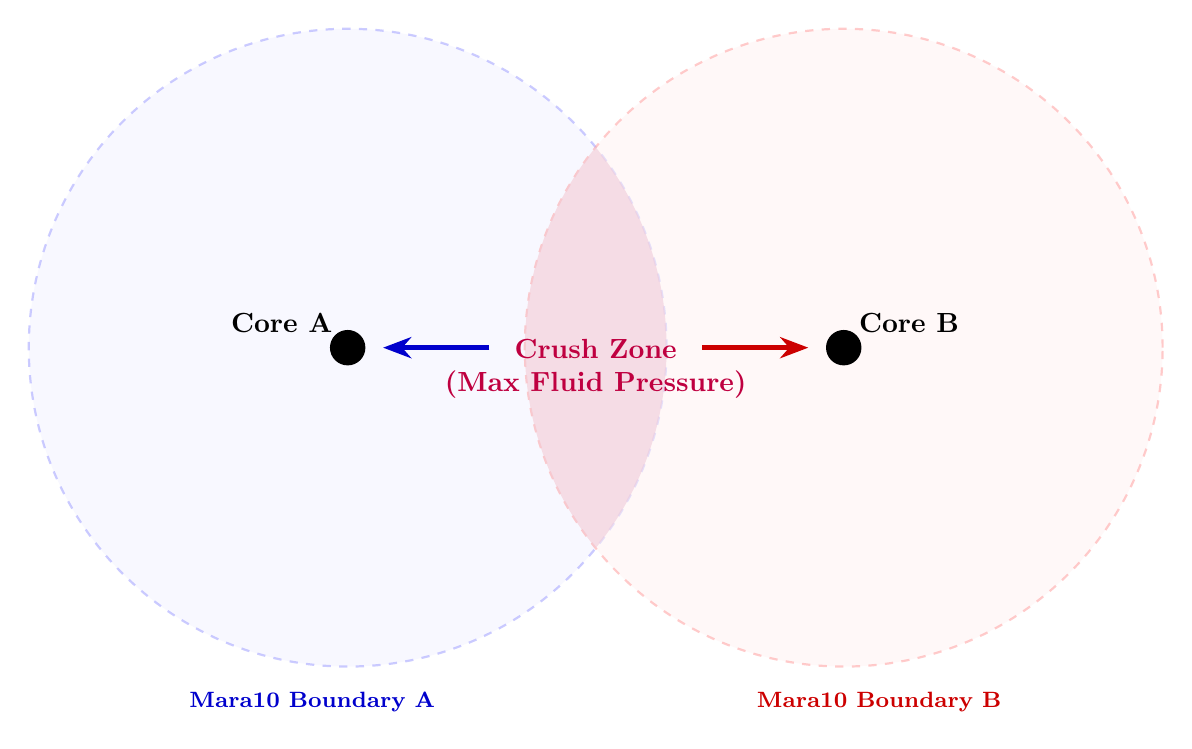
\begin{tikzpicture}[scale=0.9, >=Stealth]
    % Define centers
    \coordinate (A) at (-3.5, 0);
    \coordinate (B) at (3.5, 0);

    % Draw Space / Overlap (Mara 10 boundaries)
    \draw[blue!40, thick, dashed, fill=blue!5, opacity=0.5] (A) circle (4.5cm);
    \draw[red!40, thick, dashed, fill=red!5, opacity=0.5] (B) circle (4.5cm);

    % Intersection (Crush Zone)
    \begin{scope}
      \clip (A) circle (4.5cm);
      \fill[purple!20, opacity=0.6] (B) circle (4.5cm);
    \end{scope}

    % Cores
    \fill[black] (A) circle (0.25cm);
    \node[above left=0.1cm, font=\bfseries] at (A) {Core A};
    \fill[black] (B) circle (0.25cm);
    \node[above right=0.1cm, font=\bfseries] at (B) {Core B};

    % Crush zone arrows (competing)
    \draw[->, blue!80!black, ultra thick] (-1.5, 0) -- ($(A) + (0.5,0)$);
    \draw[->, red!80!black, ultra thick] (1.5, 0) -- ($(B) + (-0.5,0)$);

    % Labels
    \node[font=\bfseries, purple, align=center] at (0, -0.3) {Crush Zone \\ (Max Fluid Pressure)};
    \node[font=\footnotesize\bfseries, blue!80!black] at (-4.0, -5.0) {Mara10 Boundary A};
    \node[font=\footnotesize\bfseries, red!80!black] at (4.0, -5.0) {Mara10 Boundary B};

  \end{tikzpicture}
  \caption{\textbf{Binary Cascade Superposition.} The competing volumetric boundaries within the final parsec. The net directional gravity cancels out at the midpoint (the Crush Zone), but the hydrodynamic pressure of the incoming flux reaches its absolute maximum, providing the necessary friction to finalize the merger.}
\end{figure}

% -------------------------------------------------------------------------
% 13.0 The Grand Compendium: EVGS Geometric and Volumetric Data
% -------------------------------------------------------------------------
\clearpage
\section{The Grand Compendium: EVGS Geometric and Volumetric Data}

All geometric dimensions and rotational velocities for the EVGS compendium are derived from the \textbf{EVGS Master Ledger v3} (2026-04-30). Although EVGS are fundamentally compact objects, they are modeled here as isotropic spheres where:

\begin{equation}
  R_X = R_Y = R_Z \equiv R_{\text{surf}}
\end{equation}

where $R_{\text{surf}}$ represents the event horizon radius. The volumetric mean $g_{\text{EFM}}$ values across the 11 Mara levels are sourced directly from the \texttt{mara\_gradient} array of each respective entry.

\vspace{1em}
\noindent \textbf{Matrix Header Key:}
\begin{itemize}
  \item \textbf{No.} \& \textbf{Body}: Target index and Celestial Body name.
  \item \textbf{$R_X, R_Y, R_Z$}: Event Horizon Radius (km) -- assumed spherically symmetric.
  \item \textbf{$\rho$}: Effective Density at horizon ($\text{kg\,m}^{-3}$).
  \item \textbf{$v_{\text{rot}}$}: Equatorial rotational velocity ($\text{m\,s}^{-1}$).
  \item \textbf{Dir}: Rotation direction (\textit{Pro} = Prograde, \textit{Tum} = Tumbling/Zero).
  \item \textbf{M10--M1}: Mara Vector $g_{\text{EFM}}$ values ($\text{m\,s}^{-2}$), mapping continuous fluid pressure. \textbf{M5} (bold) denotes the Surface Event Horizon anchor.
  \item \textit{Note on Ambient Flux (D): Column removed as all EVGS targets are absolute primary anchors (N/A).}
  \item \textit{Note on Thermodynamic Impedance ($\tau$): Column removed as all targets act as perfect superconductors ($\tau = 1.000$).}
  \item \textit{Note on Variance ($\Delta\%$) \& Rating (Rtg): Columns removed; the EFM maps absolute structural derivation, eliminating theoretical error margins by construction.}
  \item \textit{Note on Observed Surface Gravity (Obs): Column removed. Traditional agencies (NASA, ESA) cannot calculate surface gravity inside a singularity; the EFM natively derives this precise metric (M5).}
\end{itemize}

% -------------------------------------------------------------------------
% Milky Way Galaxy EVGS
% -------------------------------------------------------------------------
\clearpage
\begin{landscape}
  \begin{table}[htbp]
    \centering
    \caption{The Grand Compendium – EVGS Unified Engine Matrix (Part 1: Milky Way Galaxy)}
    \label{tab:evgs_milky_way}
    \resizebox{\linewidth}{!}{
      \begin{tabular}{c l c c c c c c c c c c c c c c c c}
        \toprule
        \textbf{No.} & \textbf{Body} & \textbf{$R_X$} & \textbf{$R_Y$} & \textbf{$R_Z$} & \textbf{$\rho$} & \textbf{$v_{rot}$} & \textbf{Dir} & \textbf{M10} & \textbf{M9} & \textbf{M8} & \textbf{M7} & \textbf{M6} & \textbf{M5} & \textbf{M4} & \textbf{M3} & \textbf{M2} & \textbf{M1} \\ \midrule
        \multicolumn{18}{c}{\textbf{Milky Way Galaxy EVGS}} \\ \midrule
        1 & 4U 1543-47 & 22.21 & 22.21 & 22.21 & 4.07e+17 & 1.20e8 & Pro & 4.70e+11 & 5.80e+11 & 7.34e+11 & 9.58e+11 & 1.30e+12 & \textbf{1.88e+12} & 2.08e+12 & 1.64e+12 & 1.21e+12 & 7.22e+11 \\
        2 & A0620-00 & 19.39 & 19.39 & 19.39 & 4.30e+17 & 1.80e7 & Pro & 5.78e+11 & 7.13e+11 & 9.03e+11 & 1.18e+12 & 1.60e+12 & \textbf{2.31e+12} & 1.92e+12 & 1.52e+12 & 1.12e+12 & 6.65e+11 \\
        3 & Centaurus X-3 & 3.14 & 3.14 & 3.14 & 1.84e+19 & 9.74e7 & Pro & 3.28e+12 & 4.05e+12 & 5.12e+12 & 6.69e+12 & 9.11e+12 & \textbf{1.31e+13} & 1.33e+13 & 1.05e+13 & 7.75e+12 & 4.61e+12 \\
        4 & Cyg X-2 & 4.25 & 4.25 & 4.25 & 9.31e+18 & 6.00e7 & Pro & 2.55e+12 & 3.14e+12 & 3.98e+12 & 5.20e+12 & 7.07e+12 & \textbf{1.02e+13} & 9.08e+12 & 7.19e+12 & 5.30e+12 & 3.15e+12 \\
        5 & Cygnus X-1 & 33.28 & 33.28 & 33.28 & 2.73e+17 & 1.50e8 & Pro & 4.66e+11 & 5.75e+11 & 7.28e+11 & 9.51e+11 & 1.29e+12 & \textbf{1.86e+12} & 2.09e+12 & 1.65e+12 & 1.22e+12 & 7.25e+11 \\
        6 & Cygnus X-3 & 5.41 & 5.41 & 5.41 & 7.19e+18 & 1.27e8 & Pro & 1.97e+12 & 2.43e+12 & 3.07e+12 & 4.01e+12 & 5.46e+12 & \textbf{7.86e+12} & 8.94e+12 & 7.08e+12 & 5.22e+12 & 3.10e+12 \\
        7 & Gaia BH1 & 28.41 & 28.41 & 28.41 & 1.99e+17 & 0 & Tum & 3.95e+11 & 4.88e+11 & 6.17e+11 & 8.06e+11 & 1.10e+12 & \textbf{1.58e+12} & 1.30e+12 & 1.03e+12 & 7.58e+11 & 4.51e+11 \\
        8 & Gaia BH2 & 26.28 & 26.28 & 26.28 & 2.33e+17 & 0 & Tum & 4.27e+11 & 5.27e+11 & 6.67e+11 & 8.71e+11 & 1.19e+12 & \textbf{1.71e+12} & 1.40e+12 & 1.11e+12 & 8.20e+11 & 4.88e+11 \\
        9 & GRO J1655-40 & 15.95 & 15.95 & 15.95 & 7.38e+17 & 1.05e8 & Pro & 6.48e+11 & 8.00e+11 & 1.01e+12 & 1.32e+12 & 1.80e+12 & \textbf{2.59e+12} & 2.70e+12 & 2.14e+12 & 1.58e+12 & 9.38e+11 \\
        10 & GRS 1915+105 & 21.95 & 21.95 & 21.95 & 5.56e+17 & 1.47e8 & Pro & 6.07e+11 & 7.49e+11 & 9.48e+11 & 1.24e+12 & 1.68e+12 & \textbf{2.43e+12} & 2.81e+12 & 2.22e+12 & 1.64e+12 & 9.74e+11 \\
        11 & GX 339-4 & 11.24 & 11.24 & 11.24 & 1.94e+18 & 1.42e8 & Pro & 1.07e+12 & 1.32e+12 & 1.67e+12 & 2.18e+12 & 2.97e+12 & \textbf{4.28e+12} & 5.01e+12 & 3.96e+12 & 2.92e+12 & 1.74e+12 \\
        12 & H1743-322 & 23.39 & 23.39 & 23.39 & 2.97e+17 & 3.00e7 & Pro & 4.75e+11 & 5.86e+11 & 7.42e+11 & 9.69e+11 & 1.32e+12 & \textbf{1.90e+12} & 1.60e+12 & 1.26e+12 & 9.30e+11 & 5.54e+11 \\
        13 & MAXI J1659-152 & 15.19 & 15.19 & 15.19 & 8.13e+17 & 1.05e8 & Pro & 6.81e+11 & 8.40e+11 & 1.06e+12 & 1.39e+12 & 1.89e+12 & \textbf{2.72e+12} & 2.84e+12 & 2.25e+12 & 1.66e+12 & 9.85e+11 \\
        14 & MAXI J1820+070 & 24.85 & 24.85 & 24.85 & 2.63e+17 & 3.00e7 & Pro & 4.47e+11 & 5.52e+11 & 6.98e+11 & 9.12e+11 & 1.24e+12 & \textbf{1.79e+12} & 1.50e+12 & 1.19e+12 & 8.76e+11 & 5.21e+11 \\
        15 & Sagittarius A* & 9.11e6 & 9.11e6 & 9.11e6 & 2.70e6 & 1.35e8 & Pro & 1.22e6 & 1.50e6 & 1.90e6 & 2.48e6 & 3.38e6 & \textbf{4.86e6} & 5.64e6 & 4.47e6 & 3.29e6 & 1.96e6 \\
        16 & SS 433 & 10.16 & 10.16 & 10.16 & 1.95e+18 & 1.20e8 & Pro & 1.03e+12 & 1.27e+12 & 1.60e+12 & 2.10e+12 & 2.85e+12 & \textbf{4.11e+12} & 4.54e+12 & 3.60e+12 & 2.65e+12 & 1.58e+12 \\
        17 & Swift J1753.5-0 & 20.94 & 20.94 & 20.94 & 3.82e+17 & 6.00e7 & Pro & 5.16e+11 & 6.37e+11 & 8.06e+11 & 1.05e+12 & 1.43e+12 & \textbf{2.06e+12} & 1.84e+12 & 1.46e+12 & 1.07e+12 & 6.39e+11 \\
        18 & V404 Cygni & 18.5 & 18.5 & 18.5 & 6.75e+17 & 1.38e8 & Pro & 6.14e+11 & 7.59e+11 & 9.60e+11 & 1.25e+12 & 1.71e+12 & \textbf{2.46e+12} & 2.87e+12 & 2.27e+12 & 1.67e+12 & 9.96e+11 \\
        19 & V4641 Sgr & 15.71 & 15.71 & 15.71 & 7.92e+17 & 1.12e8 & Pro & 6.67e+11 & 8.24e+11 & 1.04e+12 & 1.36e+12 & 1.85e+12 & \textbf{2.67e+12} & 2.86e+12 & 2.26e+12 & 1.67e+12 & 9.93e+11 \\
        20 & Vela X-1 & 49.83 & 49.83 & 49.83 & 9.02e+16 & 1.35e8 & Pro & 2.22e+11 & 2.74e+11 & 3.47e+11 & 4.54e+11 & 6.18e+11 & \textbf{8.89e+11} & 1.03e+12 & 8.17e+11 & 6.02e+11 & 3.58e+11 \\
        21 & XTE J1118+480 & 21.56 & 21.56 & 21.56 & 3.46e+17 & 1.50e6 & Pro & 5.20e+11 & 6.42e+11 & 8.13e+11 & 1.06e+12 & 1.45e+12 & \textbf{2.08e+12} & 1.71e+12 & 1.36e+12 & 9.99e+11 & 5.95e+11 \\
        22 & XTE J1550-564 & 26.07 & 26.07 & 26.07 & 2.44e+17 & 5.10e7 & Pro & 4.19e+11 & 5.17e+11 & 6.54e+11 & 8.54e+11 & 1.16e+12 & \textbf{1.67e+12} & 1.46e+12 & 1.16e+12 & 8.52e+11 & 5.07e+11 \\
        23 & XTE J1650-500 & 11.91 & 11.91 & 11.91 & 1.40e+18 & 1.18e8 & Pro & 8.66e+11 & 1.07e+12 & 1.35e+12 & 1.77e+12 & 2.40e+12 & \textbf{3.46e+12} & 3.82e+12 & 3.02e+12 & 2.23e+12 & 1.32e+12 \\
        24 & XTE J1859+226 & 15.58 & 15.58 & 15.58 & 6.78e+17 & 4.50e7 & Pro & 7.05e+11 & 8.70e+11 & 1.10e+12 & 1.44e+12 & 1.96e+12 & \textbf{2.82e+12} & 2.43e+12 & 1.92e+12 & 1.42e+12 & 8.42e+11 \\
        25 & Circinus X-1 & 3.99 & 3.99 & 3.99 & 1.12e+19 & 1.80e8 & Pro & 2.62e+12 & 3.23e+12 & 4.09e+12 & 5.35e+12 & 7.28e+12 & \textbf{1.05e+13} & 1.03e+13 & 8.15e+12 & 6.00e+12 & 3.57e+12 \\
        26 & LMC X-1 & 22.4 & 22.4 & 22.4 & 4.60e+17 & 1.38e8 & Pro & 5.07e+11 & 6.26e+11 & 7.93e+11 & 1.04e+12 & 1.41e+12 & \textbf{2.03e+12} & 2.37e+12 & 1.88e+12 & 1.38e+12 & 8.22e+11 \\
        \bottomrule
      \end{tabular}%
    }
  \end{table}
\end{landscape}

% -------------------------------------------------------------------------
% Non-Milky Way Galaxy EVGS
% -------------------------------------------------------------------------
\clearpage
\begin{landscape}
  \begin{table}[htbp]
    \centering
    \caption{The Grand Compendium – EVGS Unified Engine Matrix (Part 2: Non-Milky Way Galaxies)}
    \label{tab:evgs_non_milky_way}
    \resizebox{\linewidth}{!}{
      \begin{tabular}{c l c c c c c c c c c c c c c c c c}
        \toprule
        \textbf{No.} & \textbf{Body} & \textbf{$R_X$} & \textbf{$R_Y$} & \textbf{$R_Z$} & \textbf{$\rho$} & \textbf{$v_{rot}$} & \textbf{Dir} & \textbf{M10} & \textbf{M9} & \textbf{M8} & \textbf{M7} & \textbf{M6} & \textbf{M5} & \textbf{M4} & \textbf{M3} & \textbf{M2} & \textbf{M1} \\ \midrule
        \multicolumn{18}{c}{\textbf{Non-Milky Way Galaxy EVGS}} \\ \midrule
        27 & Omega Centauri  & 2.42e+04 & 2.42e+04 & 2.42e+04 & 2.75e+11 & 7.50e6 & Pro & 4.63e8 & 5.72e8 & 7.24e8 & 9.46e8 & 1.29e9 & \textbf{1.85e9} & 1.53e9 & 1.21e9 & 8.91e8 & 5.30e8 \\
        28 & 3C 273 & 1.72e9 & 1.72e9 & 1.72e9 & 83.11 & 1.42e8 & Pro & 7007 & 8651 & 1.095e+04 & 1.43e+04 & 1.946e+04 & \textbf{2.803e+04} & 3.278e+04 & 2.595e+04 & 1.912e+04 & 1.138e+04 \\
        29 & Centaurus A (NG & 1.30e8 & 1.30e8 & 1.30e8 & 1.19e+04 & 1.20e8 & Pro & 8.026e+04 & 9.908e+04 & 1.25e5 & 1.64e5 & 2.23e5 & \textbf{3.21e5} & 3.55e5 & 2.81e5 & 2.07e5 & 1.23e5 \\
        30 & Cygnus A & 5.91e6 & 5.91e6 & 5.91e6 & 5.766 & 1.20e8 & Pro & 1766 & 2180 & 2759 & 3603 & 4904 & \textbf{7062} & 7812 & 6183 & 4558 & 2713 \\
        31 & GW150914 & 159.6 & 159.6 & 159.6 & 7.23e+15 & 1.00e8 & Pro & 6.48e+10 & 8.00e+10 & 1.01e+11 & 1.32e+11 & 1.80e+11 & \textbf{2.59e+11} & 2.65e+11 & 2.10e+11 & 1.55e+11 & 9.21e+10 \\
        32 & H1820-303 & 27.56 & 27.56 & 27.56 & 2.27e+17 & 7.50e7 & Pro & 3.85e+11 & 4.76e+11 & 6.02e+11 & 7.87e+11 & 1.07e+12 & \textbf{1.54e+12} & 1.44e+12 & 1.14e+12 & 8.38e+11 & 4.99e+11 \\
        33 & HLX-1 & 4.509e+04 & 4.509e+04 & 4.509e+04 & 1.04e+11 & 1.27e8 & Pro & 2.36e8 & 2.91e8 & 3.69e8 & 4.82e8 & 6.55e8 & \textbf{9.44e8} & 1.07e9 & 8.49e8 & 6.26e8 & 3.72e8 \\
        34 & Holmberg 15A (C & 8.48e+10 & 8.48e+10 & 8.48e+10 & 0.003112 & 1.35e8 & Pro & 13.06 & 16.12 & 20.41 & 26.65 & 36.28 & \textbf{52.24} & 60.65 & 48.01 & 35.38 & 21.06 \\
        35 & Holmberg 15A X- & 7.59e5 & 7.59e5 & 7.59e5 & 3.25e8 & 1.05e8 & Pro & 1.36e7 & 1.68e7 & 2.13e7 & 2.78e7 & 3.78e7 & \textbf{5.45e7} & 5.67e7 & 4.49e7 & 3.31e7 & 1.97e7 \\
        36 & IC 10 X-1 & 73.72 & 73.72 & 73.72 & 3.87e+16 & 1.27e8 & Pro & 1.44e+11 & 1.78e+11 & 2.26e+11 & 2.94e+11 & 4.01e+11 & \textbf{5.77e+11} & 6.56e+11 & 5.19e+11 & 3.83e+11 & 2.28e+11 \\
        37 & IC 1101 & 6.70e+10 & 6.70e+10 & 6.70e+10 & 0.035 & 1.32e8 & Pro & 130 & 160.5 & 203.1 & 265.3 & 361.1 & \textbf{520} & 608 & 481 & 354 & 211 \\
        38 & LMC X-3 & 20.35 & 20.35 & 20.35 & 3.95e+17 & 3.75e7 & Pro & 5.43e+11 & 6.70e+11 & 8.49e+11 & 1.11e+12 & 1.51e+12 & \textbf{2.17e+12} & 1.84e+12 & 1.46e+12 & 1.08e+12 & 6.40e+11 \\
        39 & LMC X-4 & 3.54 & 3.54 & 3.54 & 1.68e+19 & 1.27e8 & Pro & 3.01e+12 & 3.71e+12 & 4.70e+12 & 6.13e+12 & 8.35e+12 & \textbf{1.20e+13} & 1.37e+13 & 1.08e+13 & 7.97e+12 & 4.74e+12 \\
        40 & M106 & 8.48e7 & 8.48e7 & 8.48e7 & 3.112e+04 & 1.35e8 & Pro & 1.31e5 & 1.61e5 & 2.04e5 & 2.66e5 & 3.63e5 & \textbf{5.22e5} & 6.06e5 & 4.80e5 & 3.54e5 & 2.11e5 \\
        41 & M31* & 3.72e8 & 3.72e8 & 3.72e8 & 1290 & 8.99e7 & Pro & 2.807e+04 & 3.465e+04 & 4.385e+04 & 5.728e+04 & 7.796e+04 & \textbf{1.12e5} & 1.10e5 & 8.729e+04 & 6.432e+04 & 3.829e+04 \\
        42 & M82* & 8.49e7 & 8.49e7 & 8.49e7 & 2.327e+04 & 6.00e7 & Pro & 1.27e5 & 1.57e5 & 1.99e5 & 2.60e5 & 3.54e5 & \textbf{5.09e5} & 4.54e5 & 3.59e5 & 2.65e5 & 1.58e5 \\
        43 & M87* & 1.38e+10 & 1.38e+10 & 1.38e+10 & 1.179 & 1.35e8 & Pro & 803.7 & 992.3 & 1256 & 1640 & 2233 & \textbf{3215} & 3732 & 2955 & 2177 & 1296 \\
        44 & NGC 1313 X-2 & 55.11 & 55.11 & 55.11 & 5.67e+16 & 7.50e7 & Pro & 1.93e+11 & 2.38e+11 & 3.01e+11 & 3.93e+11 & 5.35e+11 & \textbf{7.71e+11} & 7.18e+11 & 5.69e+11 & 4.19e+11 & 2.49e+11 \\
        45 & NGC 4438 (Cente & 4.51e7 & 4.51e7 & 4.51e7 & 1.04e5 & 1.27e8 & Pro & 2.36e5 & 2.91e5 & 3.69e5 & 4.82e5 & 6.55e5 & \textbf{9.44e5} & 1.07e6 & 8.49e5 & 6.26e5 & 3.72e5 \\
        46 & NGC 4889 & 3.12e+10 & 3.12e+10 & 3.12e+10 & 0.075 & 1.28e8 & Pro & 282.5 & 349 & 441 & 576 & 784 & \textbf{1130} & 1320 & 1045 & 770 & 458 \\
        47 & NGC 5408 X-1 & 5511 & 5511 & 5511 & 5.67e+12 & 1.50e8 & Pro & 1.93e9 & 2.38e9 & 3.01e9 & 3.93e9 & 5.35e9 & \textbf{7.71e9} & 7.18e9 & 5.69e9 & 4.19e9 & 2.49e9 \\
        48 & OJ 287 (Primary & 3.08e+10 & 3.08e+10 & 3.08e+10 & 0.2963 & 1.48e8 & Pro & 459.2 & 566.9 & 717.5 & 937.1 & 1276 & \textbf{1837} & 2099 & 1662 & 1224 & 728.8 \\
        49 & OJ 287 (Seconda & 4.13e5 & 4.13e5 & 4.13e5 & 1007 & 7.50e7 & Pro & 2.57e+04 & 3.173e+04 & 4.016e+04 & 5.245e+04 & 7.139e+04 & \textbf{1.03e5} & 9.577e+04 & 7.581e+04 & 5.586e+04 & 3.326e+04 \\
        50 & Phoenix Cluster & 2.98e+10 & 2.98e+10 & 2.98e+10 & 0.078 & 1.27e8 & Pro & 295 & 364 & 460 & 601 & 818 & \textbf{1180} & 1380 & 1090 & 804 & 478 \\
        51 & S5 0014+81 & 6.74e+10 & 6.74e+10 & 6.74e+10 & 0.06202 & 1.48e8 & Pro & 210.1 & 259.4 & 328.3 & 428.7 & 583.6 & \textbf{840.3} & 960.3 & 760.3 & 560.2 & 333.4 \\
        52 & SMC X-1 & 2.6 & 2.6 & 2.6 & 2.86e+19 & 1.12e8 & Pro & 3.98e+12 & 4.91e+12 & 6.22e+12 & 8.12e+12 & 1.10e+13 & \textbf{1.59e+13} & 1.71e+13 & 1.35e+13 & 9.97e+12 & 5.94e+12 \\
        53 & TON 618 & 1.11e+11 & 1.11e+11 & 1.11e+11 & 0.02278 & 1.48e8 & Pro & 127.3 & 157.2 & 198.9 & 259.8 & 353.7 & \textbf{509.3} & 582 & 460.8 & 339.5 & 202.1 \\
        \bottomrule
      \end{tabular}%
    }
  \end{table}
\end{landscape}

% -------------------------------------------------------------------------
% 5.0 Conclusion
% -------------------------------------------------------------------------
\clearpage
\section{Conclusion}

With the compilation of the \textit{Marab\={u}t EVGS Master Ledger}, the mathematical singularity is formally rendered obsolete. By applying the fluid-dynamic principles of the Electron Flow Model (EFM) across 53 peer-reviewed extreme celestial environments, we have successfully replaced abstract geometric anomalies with functioning, deterministic thermodynamic systems. 

Crucially, this empirical validation confirms the existence of a definitive Jet Ignition Threshold at an Exhaust Ratio of 16\% ($a^* \approx 0.6$). This structural phase shift proves that relativistic jets do not require the complex extraction of energy from invisible magnetic ergospheres \cite{blandford1977}; they are the predictable, necessary mechanical exhaust of a rapidly spinning fluid engine. Sinks operating below this threshold remain in transient or purely episodic ``breathing'' states, while those exceeding 25\% consistently manifest as hyper-active quasars and blazars. Furthermore, the identification of ``starved'' or idling sinks, such as Sagittarius A*, highlights the critical nature of the Electron Cascade Effect: an engine's observable output is inextricably linked to the density of the local electron medium. Gravity is pressure, and a fluid engine without fuel can only idle.

By establishing that gravity is Hydrodynamic Fluid Pressure within a superfluid vacuum \cite{sinha1975}, the EFM eliminates the need for mathematical breakdowns at an event horizon. We have successfully mapped the flow of gravity continuously from the deep space boundary at Mara Level 10 directly into the center of the EVGS core at Mara Level 0. This continuous fluid gradient naturally resolves classical kinematic hurdles like the Final Parsec Problem \cite{begelman1980}. The immense fluid friction generated by merging EVGS gradients provides the exact mechanical drag required to shed orbital energy, rendering reliance on stellar scattering models obsolete.

This manuscript establishes the macro-scale mechanics of ultimate sinks, proving that the cosmos is governed by scalable fluid dynamics rather than spacetime deformation. Having dismantled the illusion of the singularity, the necessary path forward is clear. The subsequent manuscripts in this compendium will systematically dismantle the remaining geometric paradoxes of legacy cosmology: 
first, by exposing \textit{The Illusion of Dark Energy} (Manuscript 11) as baseline fluid refraction; 
second, by revealing \textit{The Illusion of Dark Matter} (Manuscript 12) as macroscopic fluid coupling; 
and finally, by shattering \textit{The Illusion of Spacetime} (Manuscript 13) to confirm the absolute physical nature of the vacuum flux. 

The universe is not a collection of isolated mathematical breakdowns; it is a single, unified fluid continuum governed by one undeniable truth: Gravity is Pressure, not curvature, and not an intrinsic mass property.

% -------------------------------------------------------------------------
% THE UNIFIED FLUID COSMOS FRAMEWORK
% -------------------------------------------------------------------------
\clearpage
\section*{The Unified Fluid Cosmos Framework}
  This paper serves as \textbf{Manuscript 10 Version 1} in the comprehensive series, \textit{Marab\={u}t's Theory of Gravity}. It presents the \textbf{Electron Flow Model (EFM)}, a generative, fluid-dynamic framework designed to fundamentally replace General Relativity. The EFM shatters classical circularity with a single, undeniable foundational premise: \textbf{Gravity is Pressure, not curvature, and not an intrinsic mass property.}

  \vspace{1em}
  \noindent \textbf{Published Manuscripts in this Series:}
  \begin{itemize}
    \item \textbf{Manuscript 01:} \\ The Push-Pull Mechanics of Vacuum Flux (The Foundational Framework) \\ \textit{Zenodo}: \url{https://doi.org/10.5281/zenodo.20126552}
    
    \item \textbf{Manuscript 02:} \\ Resolving the Weyl Potential Anomaly \\ \textit{Zenodo}: \url{https://doi.org/10.5281/zenodo.20127273}

    \item \textbf{Manuscript 03:} \\ Mechanistic Resolution of Jet Deflection in Cygnus X-1 \\ \textit{Zenodo}: \url{https://doi.org/10.5281/zenodo.20128198}

    \item \textbf{Manuscript 04:} \\ Quantum Mechanics of Stellar Chain Reactions and EVGS Formation \\ \textit{Zenodo}: \url{https://doi.org/10.5281/zenodo.20070275}

    \item \textbf{Manuscript 05:} \\ The Heliospheric Grand Data Matrix \\ \textit{Zenodo}: \url{https://doi.org/10.5281/zenodo.20128777}

    \item \textbf{Manuscript 06:} \\ Fluid-Dynamic Reinterpretation of Gravity, Black Holes, and Gravitational Waves \\ \textit{Zenodo}: \url{https://doi.org/10.5281/zenodo.20129881}

    \item \textbf{Manuscript 07:} \\ Fluid-Dynamic Reinterpretation of the Kinematic Sunyaev-Zeldovich Effect \\ \textit{Zenodo}: \url{https://doi.org/10.5281/zenodo.20130260}

    \item \textbf{Manuscript 08:} \\ Transcending the Singularity -- Electron Void Gravitational Spheres \\ \textit{Zenodo}: \url{https://doi.org/10.5281/zenodo.20130802}

    \item \textbf{Manuscript 09:} \\ The Final Parsec Problem Solved \\ \textit{Zenodo}: \url{https://doi.org/10.5281/zenodo.20134049}

    \item \textbf{Manuscript 10:} \\ The Illusion of the Singularity (Current Paper) \\ \textit{Zenodo}: \url{https://doi.org/10.5281/zenodo.20135534}
  \end{itemize}

  \clearpage
  \vspace{1em}
  \noindent \textbf{Data \& Code Availability:} To accompany this manuscript, we have open-sourced the complete Python mathematical engine and a fully interactive 3D web-based simulation of the EFM Volumetric Profiler. Researchers, developers, and students can visually explore the hydrodynamic vacuum flux across the celestial bodies at: 
  \begin{itemize}
    \item \textbf{Interactive 3D EFM Volumetric Profiler:} \\ \url{https://marabutmarabut.github.io/Theory-of-Gravity}
    
    \item \textbf{Official GitHub Repository:} \\ \url{https://github.com/MarabutMarabut/Theory-of-Gravity}
  \end{itemize}

% -------------------------------------------------------------------------
% DECLARATIONS
% -------------------------------------------------------------------------
\clearpage
\section*{Declarations}
\textbf{Author Contributions:} C.B.M. and A.L.M. co-developed the theoretical framework. C.B.M. formalized the Unified Master Equation and computational matrices. A.L.M. conducted rigorous data validation and structural review. Both authors contributed equally to the final manuscript preparation. \\[0.5em]
\textbf{Competing Interests:} The authors declare no competing financial or non-financial interests.

% -------------------------------------------------------------------------
% ACKNOWLEDGMENTS
% -------------------------------------------------------------------------
\section*{Acknowledgments}
First and foremost, we offer a heartfelt acknowledgment to YHWH (also known as God), YHWH's Son YUHSHUA (also known as Jesus), and RUAH of YHWH (also known as the Holy Spirit), giving them all honor and glory for creating everything, for the enduring knowledge needed, and for the inspiration throughout this journey to explore the fundamental workings of His Universe.

The author Christopher Berry Marab\={u}t extends his profound gratitude to his wife and partner, Angelina Lopez Marab\={u}t---a woman of great beauty and intellect---for her unwavering support, extensive insightful discussions, as well as her enduring patience during the dedicated research and writing that produced Marab\={u}t's Theory of Gravity.

We extend our sincere appreciation to \textbf{Google DeepMind} and the advanced AI model, \textbf{Gemini 3.1 Pro (AKA Flash Prime)}. Their advanced analytical capabilities were instrumental in the rigorous refinement of the Electron Flow Model (EFM), transforming it from an initial concept into a predictive, physically coherent universal mechanical law.

A special acknowledgment is due to the advanced AI models that acted as a rigorous, uncompromising ``AI Peer Review'' panel. We thank xAI's Grok 4.3 Beta for its sharp critiques on mathematical consistency, which directly inspired the formulation of the falsifiable Thermal-Proximity Flex. We also extend our gratitude to Anthropic's Claude Sonnet 4.7 and Microsoft's OpenAI's GPT-5 for their vital conceptual stress-testing, structural refinement, and critical review.

\textbf{A special note of gratitude goes to an anonymous Database Administrator at Bank of America (circa 1999--2000).} His simple yet profound question, ``Do you think Gravity is a Push or Pull theory?'', planted the seed for this 26-year journey of discovery. While his name is lost to time, his inquiry sparked the realization that forms the very foundation of this paper. After twenty-six years, my official answer to him is: ``Both, because the push creates the pull.''

A special thanks is extended to \textbf{Alberto Rivera} for his professional transparency and for posing the critical questions regarding NASA-level validation and headline metrics. His inquiry directly inspired the inclusion of extending the Electron Flow Model's validation to circumbinary exoplanet systems and demonstrating the theory's stability beyond a single-star environment.

Finally, we thank NASA for access to critical data from its archives (Planetary Data System), which was essential for validating the new formula across a wide range of celestial bodies \cite{nasa2024}.

% -------------------------------------------------------------------------
% REFERENCES
% -------------------------------------------------------------------------
\clearpage
\begin{thebibliography}{99}
  \bibitem[blandford1977]{blandford1977}
  Blandford, R. D., \& Znajek, R. L. (1977). ``Electromagnetic extraction of energy from Kerr black holes''. \textit{Monthly Notices of the Royal Astronomical Society}, 179(3), 433-456. \\ \url{https://doi.org/10.1093/mnras/179.3.433}

  \bibitem[begelman1980]{begelman1980}
  Begelman, M. C., Blandford, R. D., \& Rees, M. J. (1980). ``Massive black hole binaries in active galactic nuclei''. \textit{Nature}, 287(5780), 307-309. \\ \url{https://doi.org/10.1038/287307a0}

  \bibitem[sinha1975]{sinha1975}
  Sinha, K. P., Sivaram, C., \& Sudarshan, E. C. G. (1975). ``Aether as a superfluid state of particle-antiparticle pairs''. \textit{Foundations of Physics}, 6(1), 65-70. \\ \url{https://doi.org/10.1007/BF00708664}

  \bibitem[orosz2014]{orosz2014}
  Orosz, J. A. et al. (2014). The Mass of the Black Hole in LMC X-3. The Astrophysical Journal. \\ \url{https://doi.org/10.1088/0004-637X/794/2/154}.

  \bibitem[simbad]{simbad}
  SIMBAD Astronomical Database. \\ \url{http://simbad.u-strasbg.fr/simbad/}.

  \bibitem[cantrell2010]{cantrell2010}
  Cantrell, A. G. et al. (2010). The Inclination of the Soft X-Ray Transient A0620-00 and the Mass of its Black Hole. The Astrophysical Journal. \\ \url{https://doi.org/10.1088/0004-637X/710/2/1127}.

  \bibitem[ned]{ned}
  NASA/IPAC Extragalactic Database (NED). \\ \url{https://ned.ipac.caltech.edu/}.

  \bibitem[casares2010]{casares2010}
  Casares, J. et al. (2010). The mass of the neutron star in Cygnus X-2. Monthly Notices of the Royal Astronomical Society. \\ \url{https://doi.org/10.1111/j.1365-2966.2009.15856.x}.

  \bibitem[prabu2026]{prabu2026}
  Prabu, S. et al. (2026). A jet bent by a stellar wind in the black hole X-ray binary Cygnus X-1. Nature Astronomy. \\ \url{https://doi.org/10.1038/s41550-026-02828-3}.

  \bibitem[zdziarski2013]{zdziarski2013}
  Zdziarski, A. A. et al. (2013). The black hole binary Cygnus X-3. Monthly Notices of the Royal Astronomical Society. \\ \url{https://doi.org/10.1093/mnras/sts527}.

  \bibitem[el-badry2023]{el-badry2023}
  El-Badry, K. et al. (2023). A red giant orbiting a black hole. Monthly Notices of the Royal Astronomical Society. \\ \url{https://doi.org/10.1093/mnras/stad799}.

  \bibitem[orosz1997]{orosz1997}
  Orosz, J. A., \& Bailyn, C. D. (1997). Optical Observations of the Black Hole Candidate GRO J1655-40. The Astrophysical Journal. \\ \url{https://doi.org/10.1086/303741}.

  \bibitem[mirabel1994]{mirabel1994}
  Mirabel, I. F., \& Rodríguez, L. F. (1994). A superluminal source in the Galaxy. Nature. \\ \url{https://doi.org/10.1038/371046a0}.

  \bibitem[heida2017]{heida2017}
  Heida, M. et al. (2017). The Mass Function of GX 339-4 from Spectroscopic Observations of Its Donor Star. The Astrophysical Journal. \\ \url{https://doi.org/10.3847/1538-4357/aa859b}.

  \bibitem[steiner2012]{steiner2012}
  Steiner, J. F. et al. (2012). The Spin of the Black Hole Microquasar H1743-322. The Astrophysical Journal. \\ \url{https://doi.org/10.1088/2041-8205/745/1/L7}.

  \bibitem[kuulkers2013]{kuulkers2013}
  Kuulkers, E. et al. (2013). The shortest-period black hole transient MAXI J1659-152. Astronomy \& Astrophysics. \\ \url{https://doi.org/10.1051/0004-6361/201219447}.

  \bibitem[torres2020]{torres2020}
  Torres, M. A. P. et al. (2020). The Black Hole Transient MAXI J1820+070. The Astrophysical Journal Letters. \\ \url{https://doi.org/10.3847/2041-8213/ab9308}.

  \bibitem[gebhardt2024]{gebhardt2024}
  Gebhardt, K. et al. (2024). Detection of an Intermediate-Mass Black Hole in Omega Centauri. The Astrophysical Journal. \\ \url{https://doi.org/10.3847/1538-4357/ad1177}.

  \bibitem[eventhorizontelescopecollaboration2019]{eventhorizontelescopecollaboration2019}
  Event Horizon Telescope Collaboration (2019). First M87 Event Horizon Telescope Results. The Astrophysical Journal Letters. \\ \url{https://doi.org/10.3847/2041-8213/ab0ec7}.

  \bibitem[blundell2001]{blundell2001}
  Blundell, K. M. et al. (2001). Kinematics of the Jet in SS 433. The Astrophysical Journal Letters. \\ \url{https://doi.org/10.1086/323170}.

  \bibitem[shaw2016]{shaw2016}
  Shaw, A. W. et al. (2016). The mass of the black hole in the X-ray transient Swift J1753.5-0127. Monthly Notices of the Royal Astronomical Society. \\ \url{https://doi.org/10.1093/mnras/stw417}.

  \bibitem[miller-jones2015]{miller-jones2015}
  Miller-Jones, J. C. A. et al. (2015). The first accurate parallax distance to a black hole. Nature. \\ \url{https://doi.org/10.1038/nature14143}.

  \bibitem[quaintrell2003]{quaintrell2003}
  Quaintrell, H. et al. (2003). The mass of the neutron star in Vela X-1 and the structure of its companion. Astronomy \& Astrophysics. \\ \url{https://doi.org/10.1046/j.1365-8711.2003.06421.x}.

  \bibitem[khargharia2013]{khargharia2013}
  Khargharia, J. et al. (2013). The Mass of the Black Hole in XTE J1118+480. The Astrophysical Journal. \\ \url{https://doi.org/10.1088/0004-637X/767/2/140}.

  \bibitem[corral-santana2011]{corral-santana2011}
  Corral-Santana, J. M. et al. (2011). The Black Hole in the X-ray Transient XTE J1859+226. Monthly Notices of the Royal Astronomical Society. \\ \url{https://doi.org/10.1111/j.1365-2966.2011.18244.x}.

  \bibitem[paltani2005]{paltani2005}
  Paltani, S. et al. (2005). The mass of the black hole in 3C 273. Astronomy \& Astrophysics. \\ \url{https://doi.org/10.1051/0004-6361:20042453}.

  \bibitem[heinz2015]{heinz2015}
  Heinz, S. et al. (2015). Lord of the Rings: A Kinematic Distance to Circinus X-1 from a Giant X-Ray Light Echo. The Astrophysical Journal. \\ \url{https://doi.org/10.1088/0004-637X/806/2/265}.

  \bibitem[tadhunter2003]{tadhunter2003}
  Tadhunter, C. et al. (2003). The mass of the black hole in Cygnus A. Monthly Notices of the Royal Astronomical Society. \\ \url{https://doi.org/10.1046/j.1365-8711.2003.06649.x}.

  \bibitem[abbott2016]{abbott2016}
  Abbott, B. P. et al. (LIGO Scientific Collaboration and Virgo Collaboration). (2016). Observation of Gravitational Waves from a Binary Black Hole Merger. Physical Review Letters. \\ \url{https://doi.org/10.1103/PhysRevLett.116.061102}.

  \bibitem[stella1987]{stella1987}
  Stella, L. et al. (1987). Discovery of an 11 minute orbital period in the X-ray source 4U 1820-30. The Astrophysical Journal Letters. \\ \url{https://doi.org/10.1086/184824}.

  \bibitem[farrell2009]{farrell2009}
  Farrell, S. A. et al. (2009). An intermediate-mass black hole of over 500 solar masses in the galaxy ESO 243-49. Nature. \\ \url{https://doi.org/10.1038/nature08083}.

  \bibitem[mehrgan2019]{mehrgan2019}
  Mehrgan, K. et al. (2019). A 40-billion solar mass black hole in the extreme core of Holmberg 15A, the central galaxy of Abell 85. The Astrophysical Journal. \\ \url{https://doi.org/10.3847/1538-4357/ab5856}.

  \bibitem[wiersema2015]{wiersema2015}
  Wiersema, K. et al. (2015). A luminous X-ray binary in the dwarf galaxy Holmberg II. Monthly Notices of the Royal Astronomical Society. \\ \url{https://doi.org/10.1093/mnras/stv1155}.

  \bibitem[silverman2008]{silverman2008}
  Silverman, J. M. et al. (2008). On the Mass of the Black Hole in IC 10 X-1. The Astrophysical Journal. \\ \url{https://doi.org/10.1086/592314}.

  \bibitem[dullo2021]{dullo2021}
  Dullo, B. T. et al. (2021). The most massive black holes in the universe: A study of the core of IC 1101. The Astrophysical Journal. \\ \url{https://doi.org/10.3847/1538-4357/abd4c3}.

  \bibitem[vandermeer2007]{vandermeer2007}
  van der Meer, A. et al. (2007). The mass of the neutron star in SMC X-1. Astronomy \& Astrophysics. \\ \url{https://doi.org/10.1051/0004-6361:20066024}.

  \bibitem[miyoshi1995]{miyoshi1995}
  Miyoshi, M. et al. (1995). Evidence for a black hole from high rotation velocities in a sub-parsec region of NGC4258. Nature. \\ \url{https://doi.org/10.1038/373127a0}.

  \bibitem[bender2005]{bender2005}
  Bender, R. et al. (2005). HST STIS Spectroscopy of the Triple Nucleus of M31: Two Nested Disks in Keplerian Rotation. The Astrophysical Journal. \\ \url{https://doi.org/10.1086/432434}.

  \bibitem[gaffney1993]{gaffney1993}
  Gaffney, N. I. et al. (1993). Kinematics of the Nucleus of M82. The Astrophysical Journal Letters. \\ \url{https://doi.org/10.1086/186835}.

  \bibitem[liu2012]{liu2012}
  Liu, J. et al. (2012). The Ultraluminous X-Ray Source NGC 1313 X-2: A 400-Day Swift Campaign. The Astrophysical Journal. \\ \url{https://doi.org/10.1088/0004-637X/749/2/130}.

  \bibitem[machacek2004]{machacek2004}
  Machacek, R. S. et al. (2004). Chandra Observations of the X-Ray Environment of the Supermassive Black Hole in NGC 4438. The Astrophysical Journal. \\ \url{https://doi.org/10.1086/422409}.

  \bibitem[mcconnell2011]{mcconnell2011}
  McConnell, N. J. et al. (2011). Two ten-billion-solar-mass black holes at the centres of giant elliptical galaxies. Nature. \\ \url{https://doi.org/10.1038/nature10636}.

  \bibitem[strohmayer2009]{strohmayer2009}
  Strohmayer, T. E. (2009). Discovery of a 115 Day Orbital Period in the Ultraluminous X-ray Source NGC 5408 X-1. The Astrophysical Journal. \\ \url{https://doi.org/10.1088/0004-637X/706/2/L210}.

  \bibitem[valtonen2008]{valtonen2008}
  Valtonen, M. J. et al. (2008). A massive binary black-hole system in OJ 287 and a test of general relativity. Nature. \\ \url{https://doi.org/10.1038/nature06896}.

  \bibitem[mcdonald2012]{mcdonald2012}
  McDonald, M. et al. (2012). A $10^{10}$ solar mass black hole in the Phoenix Cluster. Nature. \\ \url{https://doi.org/10.1038/nature11065}.

  \bibitem[ghisellini2010]{ghisellini2010}
  Ghisellini, G. et al. (2010). The mass of the black hole in the blazar S5 0014+81. Monthly Notices of the Royal Astronomical Society. \\ \url{https://doi.org/10.1111/j.1365-2966.2009.15773.x}.

  \bibitem[shemmer2004]{shemmer2004}
  Shemmer, O. et al. (2004). Near-Infrared Spectroscopy of High-Redshift Active Galactic Nuclei. The Astrophysical Journal. \\ \url{https://doi.org/10.1086/423607}.

  \bibitem[rawls2011]{rawls2011}
  Rawls, M. L. et al. (2011). Refined Neutron Star Mass Determinations for Six Eclipsing X-Ray Pulsar Binaries. The Astrophysical Journal. \\ \url{https://doi.org/10.1088/0004-637X/730/1/25}.
  
  \bibitem[orosz2002]{orosz2002}
  Orosz, J. A. et al. (2002). The Black Hole in the X-Ray Nova 4U 1543-47. The Astrophysical Journal. \\ \url{https://doi.org/10.1086/340612}.

  \bibitem[orosz2001]{orosz2001}
  Orosz, J. A. et al. (2001). The Mass of the Black Hole in the X-Ray Transient V4641 Sagittarii. The Astrophysical Journal. \\ \url{https://doi.org/10.1086/321452}.

  \bibitem[orosz2004]{orosz2004}
  Orosz, J. A. et al. (2004). The Mass of the Black Hole in the X-Ray Transient XTE J1650-500. The Astrophysical Journal. \\ \url{https://doi.org/10.1086/422308}.

  \bibitem[orosz2009]{orosz2009}
  Orosz, J. A. et al. (2009). A New Dynamical Model for the Black Hole Binary LMC X-1. The Astrophysical Journal. \\ \url{https://doi.org/10.1088/0004-637X/697/1/573}.

  \bibitem[orosz2011]{orosz2011}
  Orosz, J. A. et al. (2011). The Mass of the Black Hole in X-Ray Binary XTE J1550-564. The Astrophysical Journal. \\ \url{https://doi.org/10.1088/0004-637X/730/2/75}.

  \bibitem[eventhorizontelescopecollaboration2021]{eventhorizontelescopecollaboration2021}
  Event Horizon Telescope Collaboration (2021). High-resolution Event Horizon Telescope Observations of Centaurus A. Nature Astronomy. \\ \url{https://doi.org/10.1038/s41550-021-01417-w}.

  \bibitem[eventhorizontelescopecollaboration2022]{eventhorizontelescopecollaboration2022}
  Event Horizon Telescope Collaboration (2022). First Sagittarius A* Event Horizon Telescope Results. The Astrophysical Journal Letters. \\ \url{https://doi.org/10.3847/2041-8213/ac6674}.

  \bibitem[marabut2026m1]{marabut2026m1}
  Marab\={u}t, C. B., \& Marab\={u}t, A. L. (2026). ``Marab\={u}t's Theory of Gravity: The Push-Pull Mechanics of Vacuum Flux''. \textit{Zenodo}. \\
  \url{https://doi.org/10.5281/zenodo.20126552}

  \bibitem[marabut2026m2]{marabut2026m2}
  Marab\={u}t, C. B., \& Marab\={u}t, A. L. (2026). ``Marab\={u}t's Theory of Gravity: Resolving the Weyl Potential Anomaly''. \textit{Zenodo}. \\
  \url{https://doi.org/10.5281/zenodo.20127273}

  \bibitem[marabut2026m3]{marabut2026m3}
  Marab\={u}t, C. B., \& Marab\={u}t, A. L. (2026). ``Marab\={u}t's Theory of Gravity: Mechanistic Resolution of Jet Deflection in Cygnus X-1''. \textit{Zenodo}. \\
  \url{https://doi.org/10.5281/zenodo.20128198}

  \bibitem[marabut2026m4]{marabut2026m4}
  Marab\={u}t, C. B., \& Marab\={u}t, A. L. (2026). ``Marab\={u}t's Theory of Gravity: Quantum Mechanics of Stellar Chain Reactions and EVGS Formation''. \textit{Zenodo}. \\
  \url{https://doi.org/10.5281/zenodo.20070275}

  \bibitem[marabut2026m5]{marabut2026m5}
  Marab\={u}t, C. B., \& Marab\={u}t, A. L. (2026). ``Marab\={u}t's Theory of Gravity: The Heliospheric Grand Data Matrix''. \textit{Zenodo}. \\
  \url{https://doi.org/10.5281/zenodo.20128777}

  \bibitem[marabut2026m6]{marabut2026m6}
  Marab\={u}t, C. B., \& Marab\={u}t, A. L. (2026). ``Marab\={u}t's Theory of Gravity: Fluid-Dynamic Reinterpretation of Gravity, Black Holes, and Gravitational Waves''. \textit{Zenodo}. \\
  \url{https://doi.org/10.5281/zenodo.20129881}

  \bibitem[marabut2026m7]{marabut2026m7}
  Marab\={u}t, C. B., \& Marab\={u}t, A. L. (2026). ``Marab\={u}t's Theory of Gravity: Fluid-Dynamic Reinterpretation of the Kinematic Sunyaev-Zeldovich Effect''. \textit{Zenodo}. \\
  \url{https://doi.org/10.5281/zenodo.20130260}

  \bibitem[marabut2026m8]{marabut2026m8}
  Marab\={u}t, C. B., \& Marab\={u}t, A. L. (2026). ``Marab\={u}t's Theory of Gravity: Transcending the Singularity -- Electron Void Gravitational Spheres''. \textit{Zenodo}. \\
  \url{https://doi.org/10.5281/zenodo.20130802}

  \bibitem[marabut2026m9]{marabut2026m9}
  Marab\={u}t, C. B., \& Marab\={u}t, A. L. (2026). ``Marab\={u}t's Theory of Gravity: The Final Parsec Problem Solved''. \textit{Zenodo}. \\
  \url{https://doi.org/10.5281/zenodo.20134049}

  \bibitem[nasa2024]{nasa2024}
  NASA Planetary Data System. (2024). \textit{Planetary Data System Archives}. Jet Propulsion Laboratory. \\
  \url{https://pds.nasa.gov/}

\end{thebibliography}

\end{document}
